
\documentclass[promaster]{thesis-uestc}

\title{面向容器环境异构后端的最小工作集优化研究}{Working Set Optimization Research for Heterogeneous Backend Systems in Containerized Environments}
\synctex=1
\author{张兵帅}{Zhang Bingshuai}
\advisor{段翰聪\chinesespace 研究员}{Prof. Duan Hancong}
\school{计算机科学与工程学院}{School of Computer Science and Engineering}
\major{计算机技术}{Computer Technology}
\studentnumber{202222080514}

% require all the usepackages here
% \usepackage{algorithm2e}

%这个的作用是,如果是打印模式,需要注释下面的东西,打印空白页面,如果是电子版,取消注释

% \usepackage{xpatch}
% \xpatchcmd{\endchineseabstract}{
% \checkoddpage
% \ifoddpage
%     \blankpage
% \else
%     \newpage
% \fi
% }{}{}{\fail}
% \xpatchcmd{\endenglishabstract}{
% \checkoddpage
% \ifoddpage
%     \blankpage
% \else
%     \newpage
% \fi
% }{}{}{\fail}
% \xpatchcmd{\thesischapterexordium}{
% \checkoddpage
% \ifoddpage
%     \blankpage
% \else
%     \newpage
% \fi
% }{}{}{}
% \SetKwInOut{Input}{输入}
% \SetKwInOut{Output}{输出}
\SetKwInOut{Input}{Input}
\SetKwInOut{Output}{Output}

\begin{document}

\makecover

% This is a template of mutiple files.
% The folders chapters/ and misc/ have the related files

% abstract
	
\begin{chineseabstract}

近年来,随着机器学习、图计算和云计算等数据密集型应用的迅猛发展,系统内存容量需求急剧增长,而容器化部署所引入的虚拟化开销进一步加剧了此需求。然而,传统DRAM技术面临物理缩放限制和市场价格波动等挑战,导致内存成本持续攀升。与此同时,应用程序的内存利用率普遍偏低,存在大量冷内存。另一方面,NVMe SSD、新型非易失性存储器(Non-Volatile Memory, NVM)、计算快速链接(Compute Express Link, CXL)设备以及基于RDMA的远程内存访问等新型存储与互连技术迅速发展,为内存系统架构带来了新的机遇。此外,基于软件的内存压缩技术亦不断进步。这些新兴技术在提供更高存储容量的同时,显著降低了单位容量的成本与功耗。

在此背景下,主动将应用程序中的冷内存卸载至异构后端存储,已成为一种极具潜力的成本优化策略。该策略的核心在于:利用内核的Frontswap接口实现对异构后端存储的接入,并与内核既有的换入换出机制无缝集成;为实现主动卸载并精细化管理,通过集成CGroup机制,实现主动卸载并精确控制内存卸载规模。关键在于,整个卸载过程对用户程序完全透明,无需对应用程序进行任何修改即可实现。

针对这些问题,本文的主要工作内容和创新点如下:
\begin{itemize}
    \item 提出了一种基于内存压力的自适应主动卸载方案。该方案能够自适应不同的卸载后端性能特性与用户负载状况。基于量化的内存压力,系统能够智能决策主动卸载的内存规模。通过与CGroup内存回收机制的紧密结合,实现了对应用程序内存的精准、主动卸载。
    \item 提出了一种基于访问距离的冷热页识别算法。针对现有页面冷热识别算法倾向于回收文件页、对文件密集型应用不友好的问题,本方法基于页面访问距离,能够更准确地识别文件热页,从而提升文件密集型应用的性能。
\end{itemize}

本研究开发了相应的原型系统,并针对容器化Web应用场景进行了实验验证。实验结果表明,该系统能够有效识别不同异构后端存储架构下的容器工作集,在确保服务性能的同时,实现容器内存使用量5\%-14\%的显著降低。

\chinesekeyword{分层内存,工作集大小,内存管理,冷热页面识别}
\end{chineseabstract}
\begin{englishabstract}

In recent years, the continuous development of data-intensive applications such as machine learning, graph computing, and in-memory databases, coupled with the virtualization overhead of containerized deployment, has significantly increased system memory demands. However, traditional DRAM technology faces limitations in physical scaling and is affected by market fluctuations, leading to continuously rising costs, while application memory utilization is generally low, with a large number of cold pages. Simultaneously, emerging storage and interconnect technologies such as Non-Volatile Memory Express Solid State Drives (NVMe SSDs), Non-Volatile Memory (NVM), Compute Express Link (CXL), and RDMA (Remote Direct Memory Access)-based remote memory, as well as software memory compression techniques, provide alternative solutions with higher capacity, lower cost, and reduced power consumption for memory systems.

In this context, proactively offloading cold pages from applications to heterogeneous backends is an effective cost optimization strategy. By integrating heterogeneous offloading backends into the Linux memory reclaim mechanism, the offloading process can be made fully transparent to user programs. However, traditional Linux memory management suffers from two limitations: its reclaim policy favors file pages, negatively impacting the performance of file-intensive applications; it employs a passive reactive reclaim strategy, triggered only under memory pressure, making it difficult to leverage high-performance heterogeneous backends for proactive cold page offloading.

To address the limitations of traditional Linux memory management and fully exploit the advantages of heterogeneous storage technologies, this study proposes an adaptive proactive cold page offloading scheme for heterogeneous backends. This scheme primarily tackles two key challenges: determining the appropriate offloading scale for different heterogeneous backends; and accurately identifying cold and hot pages in the system. The core innovations of this research include:
\begin{itemize}
    \item Designing an adaptive proactive offloading mechanism based on memory pressure, which can adaptively determine the offloading scale for different heterogeneous backends. This mechanism uses the synchronous reclaim latency as a pressure indicator to achieve adaptive offloading adjustments in diverse application scenarios and, through integration with the Linux CGroup framework, precisely controls the proactive offloading of application memory.
    \item Proposing a cold and hot page identification algorithm based on reuse distance (the number of distinct pages accessed between two consecutive accesses to a page). Addressing the issue that existing page coldness/hotness identification algorithms tend to reclaim file pages, which is detrimental to the performance of file-intensive applications, this algorithm, based on page reuse distance, can more accurately identify hot file pages, thereby improving the performance of file-intensive applications.
\end{itemize}

    This research has developed a corresponding prototype system and conducted experimental validation in containerized application scenarios. The experimental results demonstrate that the system can effectively identify the offloading scale for different heterogeneous backend storage architectures, and while ensuring service performance, it achieves a significant reduction in container memory usage by 5\% to 14\% compared to baseline systems.


\englishkeyword{Tiered Memory, Reuse Distance, Hot-Cold Page Identification}

\end{englishabstract}




% table of contents
\thesistableofcontents

% thesis contents
\chapter{绪\hspace{6pt}论}

% 随着硬件技术的快速发展,以RDMA分离式内存、NVM和CXL为代表的新型技术为优化内存资源利用率提供了全新思路。这些技术能够支持将访问频率较低的冷数据迁移至低成本存储设备,并按实际需求动态换入内存,有效缓解了内存容量压力。然而,现有研究主要关注通过应用程序接口(API)实现冷数据迁移的显式管理达到最优性能,这导致未经专门优化的传统应用程序难以直接从中受益。基于Linux内核缺页中断机制的透明冷数据卸载技术为解决这一问题提供了新的途径。这种方案无需修改应用程序即可自动实现冷热数据的识别与管理,但是如何确定不同的应用负载与异构卸载后端的内存内存量,很少有人研究。本文面向异构卸载后端,提出了一种自适应的主动内存卸载方案,屏蔽用户负载和异构后端内存特性,实现内存压力感知的主动卸载。

\section{研究工作的背景与意义}

随着信息技术的迅猛发展,传统DRAM技术与新兴应用需求之间的矛盾日益突出。在工艺技术层面,DRAM面临着严峻的物理局限性挑战。Mutlu\citing{mutlu2013memory}指出,当制程工艺迈向10nm及更先进节点时,DRAM存储单元的微缩已逼近物理极限,位密度提升速率显著降低。为维持性能增长趋势,产业界不得不采用多重曝光和极紫外光刻等高复杂度制造工艺,这导致了单位存储容量的制造成本呈指数级上升。根据Patel等人\citing{patel2023xfm}的实证研究,内存系统支出已占据现代数据中心总运营成本的50\%以上,成为制约大规模计算设施扩展的关键瓶颈。此外,DRAM的周期性刷新操作所需能耗随存储容量的增长而显著攀升,这进一步加剧了计算系统的能源效率问题。

与DRAM技术发展面临瓶颈形成鲜明对比的是,现代计算范式对内存系统提出了更为严苛的需求。云计算、容器虚拟化、大规模数据分析以及深度学习等新兴计算模式呈现出显著的数据密集特征,它们对内存系统的容量、带宽、访问延迟和吞吐量等核心性能指标提出了前所未有的挑战。特别是在互联网应用规模持续扩张的背景下,数据规模呈指数级增长,这种供给能力与需求规模之间的失衡使得内存资源的高效管理与优化变得愈发重要。

然而,实际生产环境中的内存利用状况却不容乐观。Reiss等人\citing{reiss2012heterogeneity}对大规模生产集群的统计分析显示,在70\%的运行时间内,集群平均有30\%的内存处于闲置状态;而在已分配的内存中,实际使用率仅为50\%。这种"高成本,低利用"的现象主要由以下因素导致:首先,现代数据中心需要同时支持在线服务、批处理任务、数据分析等多种类型的工作负载,其资源需求和运行时长存在显著差异,导致资源分配难以优化;其次,为保证服务质量(Service Level Objective,SLO),系统通常需要按照峰值需求预留内存资源,造成非高峰期的资源闲置;最后,负载的周期性特征(如日间与夜间的访问量差异)以及任务执行的固有特性(如JVM运行时环境的内存开销)进一步加剧了内存利用率低下的问题。

新型存储和互联技术的快速发展为解决内存系统面临的挑战提供了多种的解决方案。NVMe SSD、NVM等新型存储设备显著降低了存储访问延迟,而基于RDMA的高速网络技术实现了高效的远程内存访问。同时,基于软件的内存压缩技术的成熟为提升内存密度提供了新的技术路径,这些进步为构建异构分层内存系统奠定了技术基础。具体而言,RDMA技术凭借其微秒级的访问延迟和零拷贝特性,使得远程内存访问成为可能;持久性内存则因其接近DRAM的访问速度和字节寻址能力,成为理想的冷数据存储介质。此外,内存压缩技术通过对内存数据进行实时压缩和解压缩,在保证访问性能的同时显著提升了内存的有效容量。

基于上述技术进展,通过将冷数据迁移至低成本存储设备,构建异构分层内存系统,理论上可以在保证应用性能的同时显著降低总体拥有成本(Total Cost of Ownership,TCO)。在早期计算机系统中,由于磁盘的访问延迟过高,频繁的内存换入换出操作会导致系统性能的急剧下降,因此该策略并未得到广泛应用。然而,随着新型存储和互联技术的成熟,这一方案重新成为可能。Linux内核的Frontswap接口为异构后端存储的接入提供了便利,并能与内核的swap子系统无缝集成,实现内存的透明卸载。为了实现主动卸载,可以集成CGroup机制。CGroup提供的资源限制功能可以触发内存回收,进而通过swap子系统将冷页面卸载至后端存储,从而实现对卸载过程的精确控制。

鉴于容器技术(基于CGroup实现)已成为主流部署方式,并且容器是基于 CGroup实现的。在容器化部署环境下,结合Linux内核的内存回收机制,主动地将冷内存页透明地卸载至异构存储设备,有望在保障服务质量(Quality of Service,QoS)的前提下,降低内存成本,从而进一步提高数据中心的资源利用率和经济效益。

综上所述,本研究不仅具有重要的理论价值,能够推动异构内存管理技术的发展,也为解决当前内存资源利用效率低下的实际问题提供了切实可行的技术路径,具有广阔的应用前景。

\section{国内外研究历史与现状}

\subsection{分层内存研究历史与现状}

虚拟内存技术的早期发展源于应对主存容量不足的挑战。程序运行所需的内存空间往往超过实际可用物理内存,虚拟内存通过将不常用的页面迁移至辅助存储设备来模拟更大的内存空间,这一机制有效解决了内存容量限制问题\citing{10.1145/356571.356573}。Unix系统引入的分页机制最初旨在优化内存管理效率,减少外部碎片。通过将内存划分为固定大小的页面,系统能够更灵活地进行内存分配与回收。随后,这一机制被扩展以支持虚拟内存功能,实现了页面的动态换入换出,从而形成了分层内存架构的雏形\citing{10.1145/1476793.1476834,6770405}。

尽管存储技术持续进步,但磁盘和SSD的访问速度仍显著低于主存。频繁的页面交换操作会导致系统性能显著下降。因此,优化内存管理以减少页面交换、提高主存利用率成为这一阶段的研究重点\citing{Denning1968ThrashingIC}。随着硬件设备的不断发展,分层内存技术获得了新的发展机遇。不同存储介质在延迟和带宽方面的差异,使得存储层次结构更加丰富和完善。

非易失性内存(NVM)的出现标志着内存技术的重要突破。NVM不仅具备TB级的存储容量,还拥有接近DRAM的访问延迟,使其成为存储冷数据的理想介质,为分层内存架构提供了新的可能性。学术界针对这一硬件特性开展了广泛研究。

Qureshi等人\citing{10.1145/1555754.1555760}提出使用相变存储器(PCM)作为主存,DRAM作为透明缓存的架构,类似于CPU的L3缓存,由硬件自动决定数据存放和替换策略。然而,这种硬件方法缺乏灵活性,难以针对不同应用场景进行优化,频繁的页面调度还可能导致功耗增加和设备寿命缩短。

Wang等人\citing{wang2024nvpc}开发了NVPC,一种利用NVM增强页面缓存来加速现有内核文件系统的透明加速器。NVPC包含两个主要优化:同步写入加速和缓存未命中优化。对于同步写入,NVPC采用高性能的日志结构将数据从慢速磁盘重定向到快速NVM,并利用NVM的字节可寻址特性减少写入放大。对于缓存未命中,NVPC利用NVM上的空闲空间扩展DRAM页面缓存,从而容纳更多更大的工作负载。NVPC完全作为页面缓存实现,为磁盘文件系统提供高效加速,同时对用户完全透明,并与底层文件系统完全兼容。该调度算法对同步写操作繁重的应用提升效果最为显著。

Fedorov等人\citing{10.1145/3132402.3132409}提出了一种基于Linux的交换页面管理和swap机制,充分考虑了NVM的低延迟、高并行性和优异的随机访问性能。该研究采用了更智能、更激进的预取策略,并对操作系统内核的多个方面进行了修改。这种方法在运行内存需求量大的应用程序时,能够在降低内存成本的同时,将性能保持在与纯DRAM系统相当的水平。

上述方法均通过透明卸载的方式将冷数据迁移到NVM,使得现有程序无需修改即可获得性能提升。除了上述基于透明卸载的方案外,另一类研究致力于通过NVM专用编程接口(如英特尔开发的PMDK)充分发挥NVM特性,这些工作主要集中在存储系统优化领域。

DeBrabant等人\citing{DeBrabant2014APO}研究了NVM对在线事务处理(OLTP)数据库管理系统(DBMS)架构的影响。研究者通过硬件仿真器模拟了NVM-only和NVM+DRAM两种存储架构,并使用YCSB和TPC-C基准测试,发现现有DBMS无法充分利用NVM技术,因为其内部架构基于内存易失性的假设。因此,需要针对NVM特性重新设计数据库系统。

Lindstrom等人\citing{7304362}、van Renen等人\citing{10.1145/3183713.3196897}、喻明\citing{喻明2023面向NVM和SSD的列存数据库存储引擎设计与实现}、董创轼\citing{董创轼2023基于NVM的数据库存储引擎优化技术研究}以及李心池\citing{李心池2018基于NVM的内存数据库多表连接操作的设计与优化}等研究均致力于利用NVM优化数据库性能,并取得了不同程度的性能提升。

基于RDMA的远程内存技术通过解决不同节点间内存负载不均衡的问题,实现了内存利用率的提升。Gu等人\citing{201565}提出的Infiniswap系统利用Infiniband的RDMA低延迟特性,将多个节点的远程内存作为交换空间,并将其划分为固定大小的slab进行分布式管理。通过RDMA操作实现低延迟的同步远程写入和高容错的异步磁盘写入,同时利用分布式的Infiniswap守护进程,无需中央协调即可协同管理这些远程可访问的内存,并主动监控、预分配和驱逐slab。与磁盘相比,应用程序吞吐量提高了4倍至15.4倍。

Amaro等人\citing{10.1145/3342195.3387522}提出的FastSwap系统进一步优化了基于RDMA的远端内存架构。该系统通过直接与Linux的cgroup子系统交互,实现了本地内存与远端内存之间的细粒度管理。其创新之处在于引入了远端内存感知集群调度器,该调度器能够全局感知集群中的远端内存资源分布,并据此动态调整各作业的本地内存配额,确保资源利用的均衡性。实验表明,相比Infiniswap,FastSwap在资源利用效率和系统吞吐量方面均取得了显著提升。

Ruan等人\cite{ruan2020aifm}提出了一种名为AIFM的系统。该系统将交换操作与应用程序级别的内存对象绑定,以库的形式提供了一系列API。通过这些API,开发人员可以构建远程化、近远混合内存的数据结构,并根据应用程序的内存访问特征进行优化。AIFM在不牺牲性能的前提下显著增加了可用内存,在特定测试用例中,其性能比Fastswap\cite{10.1145/3342195.3387522}高出61倍。

Yoon等人\cite{yoon2021dilos,yoon2023dilos}基于库操作系统构建了Unikernel内核DILOS。DILOS通过简化缺页中断处理流程来加速内存访问,同时兼容POSIX接口,使得现有程序能够在其上运行。此外,DILOS提供了预取指导库接口,允许应用程序通过实现该接口来指导预取操作。实验结果表明,DILOS在性能上可与AIFM\cite{ruan2020aifm}相媲美。

随着硬件加速技术的发展和软件算法的优化\cite{10.1145/3620666.3651323},内存压缩技术的性能开销已显著降低。现代应用程序的数据通常具有较高的可压缩性,这使得实时压缩冷数据以扩展有效内存容量成为一种可行的方案。Google\cite{10.1145/3297858.3304053}率先在其生产环境中采用压缩内存作为交换后端,并利用机器学习技术预测工作集大小,从而实现主动卸载。这一策略显著提高了数据中心的内存利用率。

以上大部分工作\cite{10.1145/3132402.3132409,201565,10.1145/3342195.3387522,ruan2020aifm,yoon2021dilos,yoon2023dilos}均验证了在应用程序中使用分层内存的可行性,并提出了各自的成本优化方案。然而,这些方案通常依赖于经验配置工作集,缺乏对工作集进行实时、主动调整的能力。

\subsection{工作集估计算法研究历史与现状}

工作集大小(Working Set Size, WSS)是量化进程内存需求的关键指标,也是主动卸载内存的核心指标,它反映了进程在特定时间窗口内频繁访问的内存页面集合。传统Linux系统主要基于页表引用(Referenced)标志来估算WSS:通过统计被CPU访问而置位的页面数量来评估活跃内存使用量。然而,这种方法需要遍历整个页表,在处理大内存进程时会产生显著的性能开销,同时可能影响系统的整体响应性。

针对传统方法的局限性,研究者提出了多种优化方案。在虚拟化环境中,内存工作集的准确估算对于资源调度尤为重要。Vlad Nitu等人\citing{10.1145/3179422,10.1145/1165389.945462}创新性地将统计采样引入工作集估算。他们通过在Guest OS中部署气球驱动(balloon driver),选择性地使部分页面映射失效并监控重新访问行为,从而在降低扫描开销的同时获得较准确的工作集估计。基于这一思路,Anna Melekhova等人\citing{Melekhova2015EstimatingWS}对气球驱动机制进行了改进,通过VirtIO接口实现了更高效的内存使用统计收集,使得工作集估算的准确度提升。

随着数据中心规模的扩大和负载特征的日益复杂化,基于历史数据的预测方法开始受到关注。Xie等人\citing{9076292}通过分析内存使用模式的周期性特征,提出了结合ARIMA和三指数平滑的混合预测模型。该模型能够捕捉内存使用的长期趋势和短期波动,与传统方法相比,这种基于预测的方法能够提前预知工作集大小的变化,为内存资源的动态调度提供了可能。

为进一步降低监控开销,Lian等人\citing{9860164}提出了基于eBPF的轻量级工作集估计方法。通过利用eBPF技术的高效事件追踪能力,他们实现了对缺页中断、内存分配和页面访问等关键事件的非侵入式监控。结合LightGBM机器学习模型,降低算法开销,便于部署。

近年来,深度学习等先进机器学习方法在工作集估算领域展现出良好的应用前景。多项研究\citing{10.1145/3297858.3304053,9870561,10.1155/2023/5959223}探索了针对特定应用场景的深度学习模型,通过建立更复杂的特征工程和预测模型来提高估算精度。这些方法虽然在特定场景下表现优异,但其泛化能力和部署成本仍需要进一步验证。对于不同的工作负载以及卸载后端,需要设计不同的模型,迁移成本较高。


\section{本文的主要贡献与创新}

随着异构存储设备的发展,分层内存技术被广泛应用于现代数据中心。然而,现有的分层内存系统和工作集估计算法存在以下局限性:首先,多数分层内存系统仅作为概念验证,依赖于经验设定工作集大小,缺乏动态调整机制,无法实现主动内存卸载;其次,现有的工作集估计算法多基于统计或机器学习方法,但这些方法所依赖的统计数据与工作集大小之间往往呈现非线性关系,导致估计精度不足;最后,现有算法通常针对特定后端设备或应用场景进行优化,缺乏对不同负载和设备特性的自适应能力。

此外,主动卸载过程中的页面选择策略也至关重要。传统的 Linux 系统倾向于回收文件页面,但在存储后端性能大幅提升的现代异构环境中,这种策略可能导致文件密集型应用性能下降。尽管 Linux 提供了 \texttt{swappiness} 参数来调整页面回收策略,但该参数依赖于人工经验设置,无法动态适应系统性能变化。

针对上述问题,本文提出了一种面向异构卸载后端的自适应主动卸载方案。该方案能够透明地将应用程序的冷数据卸载到基于 \texttt{Frontswap} 接口的异构后端,并根据不同的用户负载和后端设备特性进行自适应调整。本文的主要贡献与创新包括:

\begin{enumerate}
    \item \textbf{基于同步内存回收性能损失的内存压力度量方法:} 与传统的基于缺页率或页面分配次数的指标不同,我们通过监控同步内存回收操作导致的应用程序性能下降程度来量化内存压力。这种方法能够更直接、准确地反映内存压力对应用程序性能的实际影响,并能够屏蔽用户负载和异构后端设备特性的差异。

    \item \textbf{基于负反馈的自适应工作集估计算法:} 我们提出了一种基于内存压力的负反馈工作集估计方法。该方法根据上述内存压力度量结果,动态调整工作集大小:当内存压力较小时,增加工作集大小以减少缺页;当内存压力较大时,减小工作集大小以触发主动卸载。通过这种负反馈机制,系统能够自动适应不同的负载和设备特性。

    \item \textbf{优化的匿名和文件页面回收策略:} 针对匿名页和文件页的回收比例不平衡问题,提出了一种新的页面访问距离计算方法。该方法能够根据实际的性能影响动态调整文件页面和匿名页面的回收比例,更好地适应现代存储设备的特性,从而提升系统整体性能,尤其是文件密集型应用的性能。
\end{enumerate}

\section{本论文的结构安排}
本文的章节结构安排如下:

\footnote{脚注序号“\ding{172},……,\ding{180}”的字体是“正文”,不是“上标”,序号与脚注内容文字之间空1个半角字符,脚注的段落格式为:单倍行距,段前空0磅,段后空0磅,悬挂缩进1.5字符;中文用宋体,字号为小五号,英文和数字用Times New Roman字体,字号为9磅;中英文混排时,所有标点符号(例如逗号“,”、括号“()”等)一律使用中文输入状态下的标点符号,但小数点采用英文状态下的样式“.”。}
\chapter{内存管理及分层内存系统概述}

\section{Linux 内存管理技术}

\subsection{物理内存管理机制}

\begin{figure}[h]
    \centering
    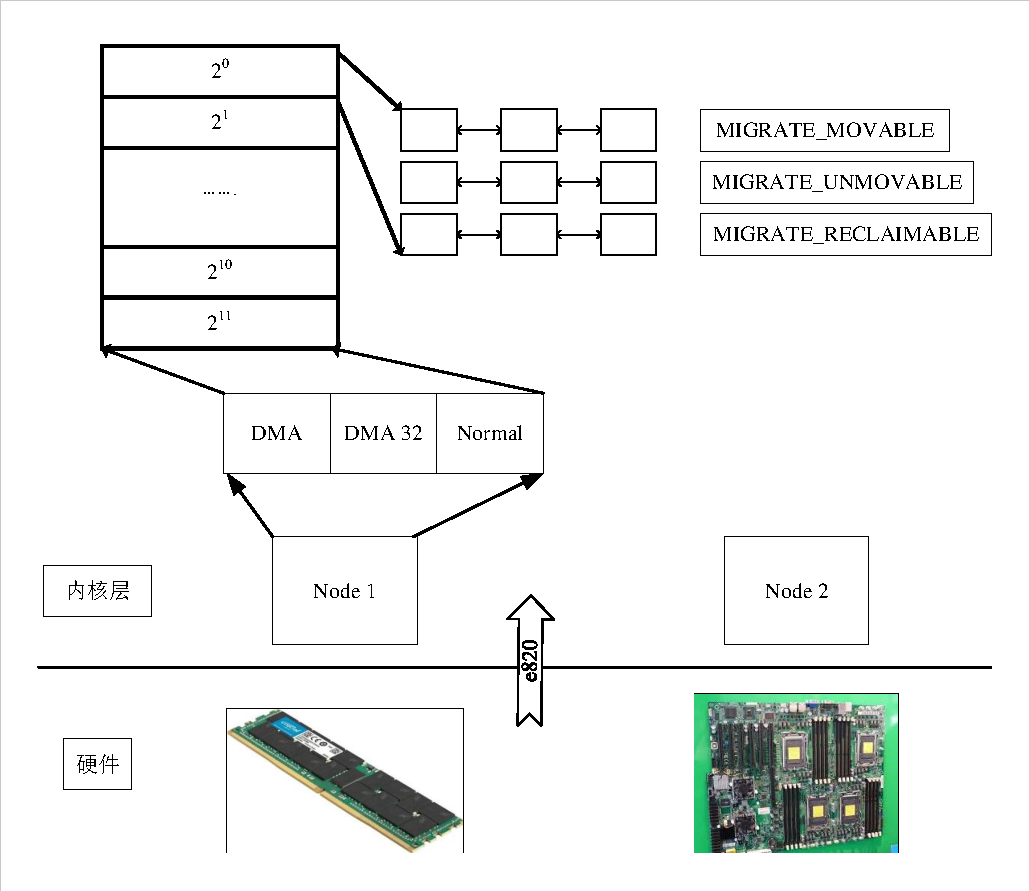
\includegraphics[width=\textwidth,keepaspectratio]{物理内存管理.pdf}
    \caption{Linux物理内存管理架构}
    \label{物理内存管理}
\end{figure}

Linux操作系统采用多层次结构管理物理内存,以实现高效的内存分配和回收。如图\ref{物理内存管理}所示,Linux物理内存管理机制从NUMA节点(Node)、内存区域(Zone)、伙伴系统(Buddy System)、页框管理(Page Frame)以及内存探测(Memory Detection)等多个层面进行组织,形成了一个完整且高效的内存管理体系。分层结构不仅能够满足不同硬件设备和软件应用的需求,还能有效降低内存碎片,提高系统整体性能。

在NUMA架构中,Linux将物理内存划分为多个节点,每个节点由 pg\_data\_t 结构表示。该结构包含多个关键成员,例如 node\_zones[] 用于存储节点内的内存区域,node\_mem\_map 指向该节点的页框描述符数组,而 node\_start\_pfn 则记录了节点的起始页帧号。这种设计使得Linux能够充分利用NUMA架构的特性,优化内存访问性能。每个节点进一步划分为多个内存区域,包括 ZONE\_DMA、ZONE\_DMA32 和 ZONE\_NORMAL。这些区域根据物理地址范围和用途进行划分,例如 ZONE\_DMA 适用于 ISA 设备的 DMA 操作,ZONE\_DMA32 适用于只能寻址 32 位内存的设备,而 ZONE\_NORMAL 则用于系统常规内存使用。每个内存区域由 struct zone 结构表示,其中 free\_area[] 用于管理伙伴系统的空闲页框链表,watermark[] 用于控制内存回收的水位线,而 lock 则用于保护并发访问。

伙伴系统是Linux物理内存分配的核心机制,它将连续物理页框组织为大小为\(2^n\)个页的块。从\(2^0\)到\(2^{11}\)的不同阶分别对应1页到2048页的连续内存块。每个阶维护一个空闲块链表,通过 struct free\_area 结构管理。struct free\_area 包含 free\_list[] 用于按迁移类型分类的空闲页链表,以及 nr\_free 用于记录该阶的空闲块数量。为了减少内存碎片,Linux定义了多种内存迁移类型,包括 MIGRATE\_UNMOVABLE(不可移动页,如内核数据结构)、MIGRATE\_MOVABLE(可移动页,如用户空间应用程序数据)和 MIGRATE\_RECLAIMABLE(可回收页,如页缓存、tmpfs等)。伙伴系统中的每个空闲区域列表按迁移类型进一步划分,这使得分配器能够优先从相同迁移类型的页框中分配内存,从而降低内存碎片。

Linux将物理内存的最小管理单位定义为页框,通常为4KB。每个页框由 struct page 结构体表示,其中 flags 用于记录页框状态标志,\_refcount 用于管理引用计数,而 lru 则用于页框回收的LRU链表。系统中的每个物理页框都由一个 struct page 实例表示,所有页框结构体组成一个连续数组,称为 mem\_map。这种设计使得Linux能够高效地管理物理内存的分配和回收。

在系统启动阶段,Linux通过e820机制探测物理内存布局。e820是BIOS提供的一种接口,用于报告可用的物理内存区域。每个e820条目由 \_\_u64 addr(内存区域起始地址)、\_\_u64 size(内存区域大小)和 \_\_u32 type(内存区域类型,如RAM、保留等)组成。内核解析e820表后,识别出可用物理内存,初始化节点和区域数据结构,并设置伙伴系统的初始状态。这种机制使得Linux能够准确识别和管理系统中的物理内存资源。

综上所述,Linux物理内存管理机制通过多层次、多维度的设计,实现了高效的物理内存管理,以满足不同硬件设备和软件应用的需求。

\subsection{虚拟内存分页机制}

\begin{figure}[h]
    \centering
    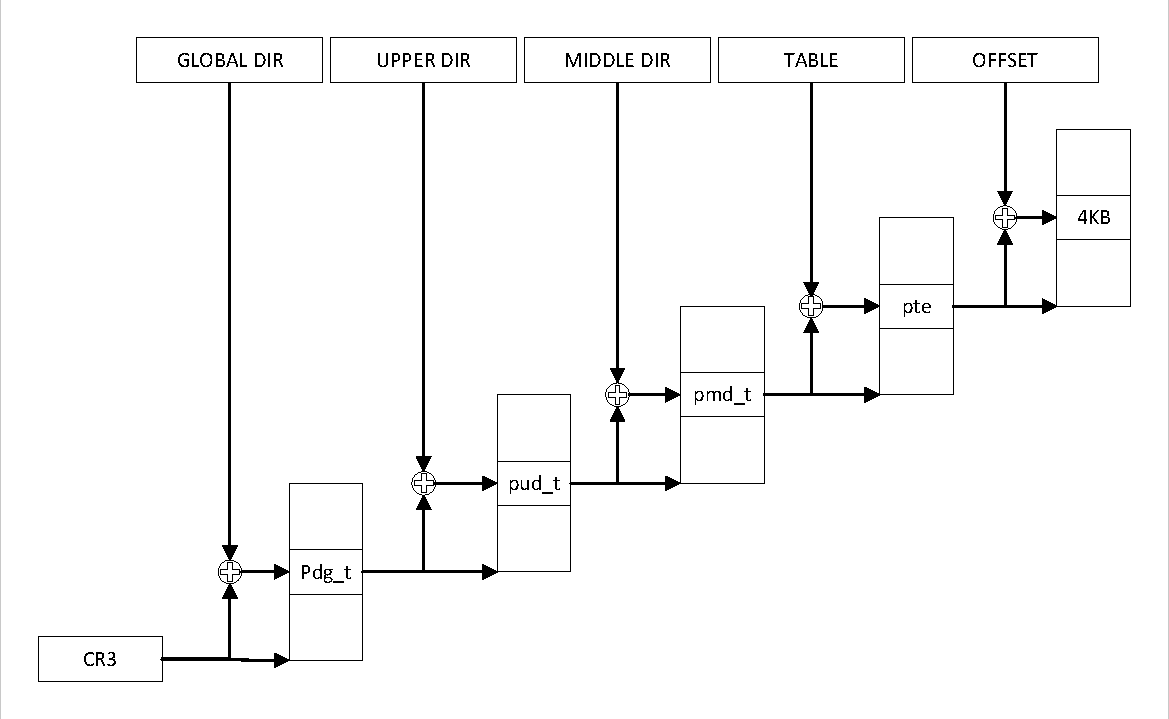
\includegraphics[width=\textwidth,keepaspectratio]{页表.pdf}
    \caption{Linux多级页表机制}
    \label{页表}
\end{figure}

Linux 内核(以 4.12.0 版本为例)采用多级分页模型来管理虚拟内存到物理内存的映射。该模型如图\ref{页表} 四种页表结构:页全局目录 (Page Global Directory,PGD)、页上级目录 (Page Upper Directory,PUD)、页中间目录 (Page Middle Directory,PMD) 和页表 (Page Table,PT)。这些页表结构以层次化的方式组织,PGD 位于层次结构的顶层,PT 位于底层。

系统的 cr3 寄存器保存了当前进程的 PGD 的物理地址。PGD 包含若干 PUD 的地址。当进程切换时,内核通过进程描述符之间的传递,将下一个要执行的进程的 PGD 地址保存在 cr3 寄存器中。这样,当新的进程获得 CPU 使用权后,cr3 寄存器就指向了该进程的页表 PGD 的物理地址。

每个 PUD 包含若干 PMD 的地址,每个 PMD 包含若干 PT 的地址,而 PT 中的每个页表项 (Page Table Entry,PTE) 最终包含了虚拟地址对应的物理页框的信息。通过分析 PTE,可以确定该虚拟地址对应的页面是位于物理内存中(及其物理地址),还是已经被换出到交换区(及其在交换区中的位置)。

进程的虚拟地址空间被划分为多个页面。当进程访问一个虚拟地址时,通过多级页表机制实现线性地址到物理地址的转换。首先,通过各级页表进行查找。如果该地址所在的页面已经被映射到物理内存,通过各级页表的表项值即可定位到页表项。然后分析页表项以及虚拟地址中的偏移量可以确定该虚拟地址所在的物理页框和偏移量;如果该虚拟地址没有被映射到物理地址,则在各级页表上可能会出现其表项信息的缺失,此时内核通过首先分配页面,然后根据该页的物理地址和其他信息综合填充到页表项中,同时也会刷新页表和块表中的内容。 对于不同的缺页异常会调用不同的方法去处理。

对于使用虚拟内存技术和缺页异常的系统,进程的线性地址空间中被划分出来的页面不必全部常驻内存。当 MMU(Memory Management Unit)在运行中进行寻址时发现某个逻辑地址对应的物理地址未被映射,说明该逻辑地址对应的页不在内存中,此时 Linux 系统采用缺页中断,将页面从磁盘读入内存。此外,还有两种情况下的页不需要常驻内存:换出到交换区的页面、只读页面发生了写操作。

Linux 系统将缺页异常分为两种类型:主缺页异常 (Major Page Fault) 和次缺页异常 (Minor Page Fault)。主缺页异常是指需要从慢速的存储设备中读取一个页的数据到内存中。

相反地,其他情况下的缺页异常被归类为次缺页异常,例如为物理页面分配一个页面帧、从交换高速缓存中删除并将页面分配给进程等。

具体来说,当发生缺页异常时,Linux 系统首先通过解读各级页表的内容以区分主缺页中断和次缺页中断。当发生主缺页异常时,说明需要从慢速存储设备中读取页面到内存中。于是调用一个与体系结构无关的顶层函数: handle\_mm\_fault() 来处理后援存储器中的缺页异常,将数据从磁盘设备读入内存并更新各级页表以及高速缓存的内容。该函数将主缺页异常分为三大类不同的情况:页面被换出到交换区、未建立页表项到物理内存的映射关系、发生了写时复制。

内核通过页表项判断出页面被换出到了交换区。它首先检查页表项的 present 位,当发现它的值为 0 时,说明页面不在内存中。此时若页表项的高位非空则说明:此缺页异常由换出到交换区的匿名页引起。内核通过解析非空的页表项得到页面在磁盘上交换区上的位置,该位置信息在页面被系统换出到交换区后根据槽位和块号码编码得到并写入了页表项。因此解码页表项后就可以得到页面所在的磁盘位置,之后将调用 do\_swap\_page() 函数来进行处理。do\_swap\_page() 在向系统申请了一个可用的物理页后,就可以向磁盘发起 I/O 请求,将页面读入内存。需要注意的是,页面并不是立即被交换出去的,而是被放到了交换高速缓存中。原因在于页面可能被多个进程所共享,当页面被放入交换高速缓存,而其他共享该页面的进程需要使用此页面时,就可以在交换高速缓存中找到,从而避免了从磁盘交换区中读取的开销。

内核也可通过页表项判断发生缺页异常的原因:逻辑地址所在的页尚未建立与物理页框之间的映射关系。此时映射关系或是匿名映射,或是文件映射。当发生匿名映射时,内核调用 do\_anonymous\_page() 方法,为进程申请一个物理页框,然后建立逻辑地址到物理地址的映射关系。内核中有一个守护进程时刻在监控系统的内存使用率,当达到阈值的时候,该进程就会将不常用的页换出到磁盘或者直接丢弃。对于匿名页而言,它们没有磁盘上的副本,因此被换出到交换区中。

\subsection{资源控制组(CGroup V2)}

Linux Control Groups (cgroups) v2 是 Linux 内核中的一个关键资源管理机制,其设计目标是提供统一、一致且高效的系统资源分配与隔离框架。cgroups v2 于2016年首次引入 Linux 内核主线,旨在解决 cgroups v1 中存在的诸多结构性问题。在系统架构层面,cgroups v2 抛弃了 v1 中允许多层级并存的复杂设计,转而采用单一层级结构,这种变化显著简化了资源管理模型并消除了控制器间的交互冲突。cgroups v2 由两个核心组件构成:cgroup 核心负责进程的层级组织;控制器则负责特定资源类型的分配与限制。与 v1 不同,cgroups v2 强制要求一个进程的所有线程必须位于同一 cgroup 中,从根本上解决了线程与内部节点之间的资源竞争问题。此外,cgroups v2 引入了资源分配模型的标准化,包括权重(weights)、限制(limits)、保护(protections)和分配(allocations)四种主要模型,为各控制器提供一致的行为基础。

cgroups v2 的用户态接口设计遵循一致性原则,通过虚拟文件系统(通常挂载于 /sys/fs/cgroup )暴露给用户空间。核心接口文件包括 cgroup.procs (列出并管理 cgroup 中的进程)、 cgroup.controllers (显示可用控制器)、 cgroup.subtree\_control (启用或禁用控制器)和 cgroup.events (提供状态变化通知)等。与 v1 相比,v2 的接口命名更加规范化,如使用 .max 表示硬限制, .high 表示软限制, .low 表示保护阈值,设计更加直观且语义明确。cgroups v2 还提供了委托机制,允许系统管理员将 cgroup 子树的管理权委托给普通用户或容器命名空间,同时保证这些委托操作不会突破上级 cgroup 设置的资源边界,为容器化环境和多租户系统提供了坚实的基础。

在内存管理方面,cgroups v2 的内存控制器实现了全面而精细的控制能力。它不仅跟踪用户空间内存(页缓存和匿名内存),还监控内核数据结构(如目录项和索引节点)、TCP 套接字缓冲区等内存使用。内存控制器引入了多层次的限制机制: memory.high 作为主要的限制阈值,当 cgroup 超过此值时,其进程会被限流并面临增强的内存回收压力,但不会直接触发 OOM 杀手; memory.max 作为硬性上限,一旦达到且无法通过回收减少使用量,则会启动 OOM 终止机制; memory.low 提供尽力而为的内存保护,当 cgroup 及其所有祖先的内存使用均低于各自的 low 值时,该 cgroup 的内存不会被系统回收。这种分层设计解决了 v1 中软限制(soft limit)实现效率低下且无层级意义的问题,同时避免了硬限制(hard limit)过于严格导致资源浪费或频繁 OOM 的困境。

cgroups v2 还增强了各控制器间的协同能力。在 v1 中,由于多层级架构,控制器之间难以协作,而 v2 中的单一层级使得控制器能够共享相同的进程组织视图,从而能够实现更复杂的资源管理策略。例如,内存控制器和 IO 控制器能够协同工作,通过脏页控制平衡内存使用与 IO 性能。此外,cgroups v2 引入了可写回(writeback)支持,允许文件系统正确地将脏页写回操作归属到适当的 cgroup,从而实现更精确的资源核算。

对于系统管理员和容器运行时实现者而言,cgroups v2 提供了更加可预测和一致的行为模型。v2 的设计理念是先组织后控制(organize once and control),鼓励用户在启动时将工作负载分配到适当的 cgroup 结构中,然后通过调整控制器配置来动态管理资源分配,而不是频繁地在 cgroup 间迁移进程。这种方法更符合现代容器化环境的需求,也避免了因进程迁移导致的性能开销和资源状态不一致问题。同时,cgroups v2 还解决了 v1 中权限模型不清晰的问题,提供了明确的权限约束,确保未授权用户无法突破限制或干扰系统资源分配。

总体而言,cgroups v2 通过结构简化、接口统一和行为标准化,为 Linux 系统提供了更加健壮和高效的资源管理框架,特别适合于现代云原生和容器化环境中的资源隔离与调度需求。

\subsection{内存回收机制}
\label{sec:Linux内存回收机制}

Linux操作系统采用层次化内存管理架构,将物理内存组织为node和zone的二级结构。为实现系统性能与内存使用效率的平衡,Linux实现了一套完善的内存回收机制,本文系统阐述其工作原理与实现细节。

\begin{figure}[h]
    \centering
    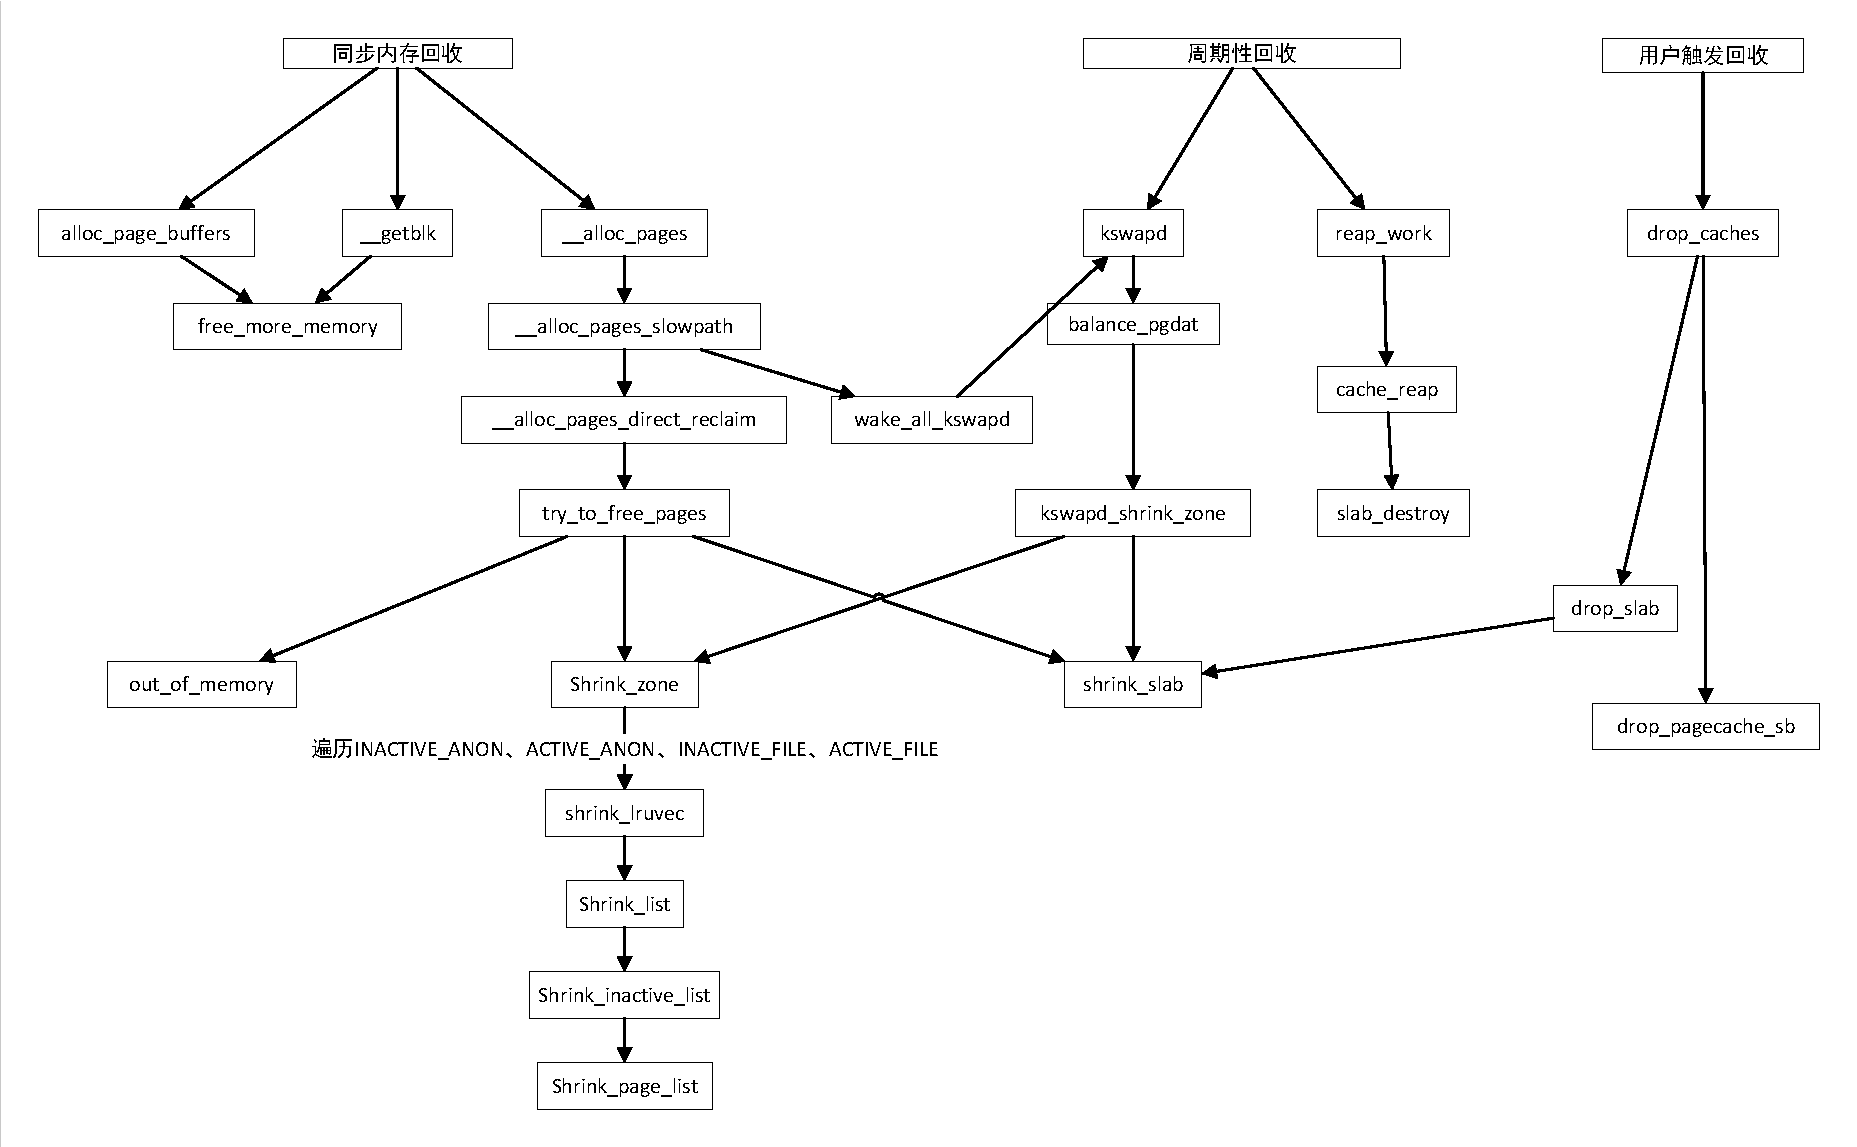
\includegraphics[width=\textwidth,keepaspectratio]{内存回收调用栈.pdf}
    \caption{内存回收调用栈}
    \label{fig:memory_reclaim_callgraph}
\end{figure}

内存回收的主要目标是在系统内存压力增大时,释放低价值页面以满足新的内存分配需求。Linux通过水位线(watermark)机制监控内存使用状况,当空闲内存低于特定阈值时触发回收。如图\ref{fig:memory_reclaim_callgraph}所示,内存回收机制主要包含以下三种策略:

\begin{itemize}
    \item 直接回收(Direct Reclaim):由内存分配失败的进程同步触发,该进程暂停执行直到回收足够内存
    \item 周期性回收(Periodic Reclaim):由kswapd守护进程在后台定期执行,维持系统内存平衡
    \item 用户触发回收(User-triggered Reclaim):通过接口允许用户主动释放缓存和不活跃内存
\end{itemize}

这三种机制虽然触发条件和路径不同,但最终都会调用相同的底层回收函数,如shrink\_active\_list、shrink\_inactive\_list和shrink\_page\_list等,形成统一的回收框架。

同步内存回收由alloc\_page\_buffers、\_\_getblk和\_\_alloc\_pages等函数触发,最终通过free\_more\_memory和\_\_alloc\_pages\_slowpath路径执行回收。周期性回收由kswapd守护进程负责,通过balance\_pgdat和kswapd\_shrink\_zone函数调整页面分配。用户触发回收则通过drop\_caches接口实现,使用drop\_slab和drop\_pagecache\_sb函数释放缓存。这三种机制最终在shrink\_active\_list、shrink\_inactive\_list和\\shrink\_page\_list等底层函数处汇合。

kswapd线程被唤醒后,以order和zone数组下标classzone\_idx为参数调用balance\_pgdat()。该函数按照normal->dma32->dma顺序扫描zone,通过zone\_balanced()判断zone是否平衡。判断依据包括:zone空闲内存超过高水位线,以及内存在0到指定order之间平衡分布(即总内存超过高水位,order-1及以上内存超过高水位的\(\frac{1}{2}\),依此类推)。系统确定第一个不平衡zone的下标为end\_zone,仅针对0至end\_zone范围执行回收,避免与其他进程的内存分配冲突。

\begin{figure}[h]
    \centering
    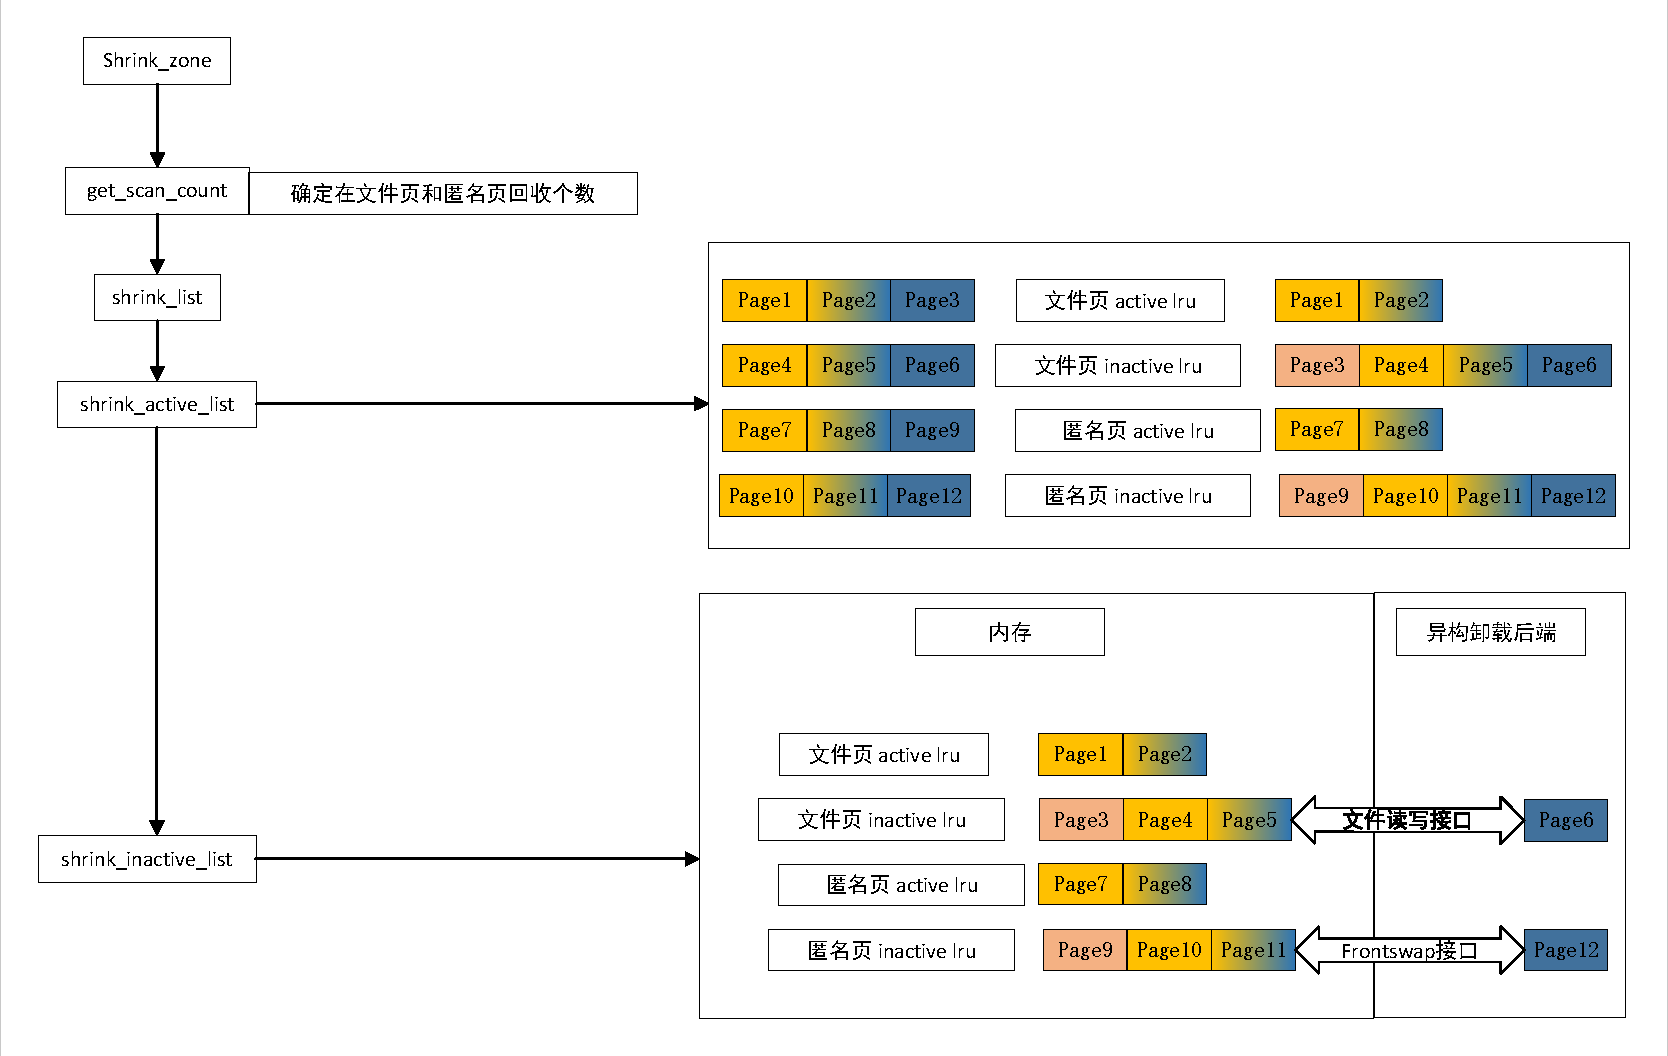
\includegraphics[width=\textwidth,keepaspectratio]{内存回收流程示意图.pdf}
    \caption{内存回收流程示意图}
    \label{fig:memory_reclaim_mechanism}
\end{figure}

如图\ref{fig:memory_reclaim_mechanism}所示,Linux内存回收机制采用精细的页面分类管理策略,通过结构化的回收流程实现高效的内存资源管理。系统维护四个LRU(最近最少使用)链表,将页面按照活跃度(active/inactive)和页面类型(匿名页/文件页)进行二维分类:active匿名页链表、inactive匿名页链表、active文件页链表和inactive文件页链表。从理论角度分析,Linux的LRU链表实现基于多队列理论(Multi-Queue Theory)的变体,针对不同类型页面的访问模式特征进行了优化。这种设计解决了传统LRU算法面临的扫描污染(Scan Pollution)问题——即顺序访问大量数据时可能会驱逐出所有热点数据。通过区分文件页和匿名页,系统能够针对性地处理不同的内存访问模式:文件页通常表现为时空局部性较强的访问模式,而匿名页则更多地呈现出工作集(Working Set)特征。

实际回收由shrink\_zone()函数执行,该函数按照以下步骤进行操作:

\begin{enumerate}
    \item shrink\_zone()首先调用get\_scan\_count()确定在文件页和匿名页中需要回收的页面数量。这一决策受到系统swappiness参数的影响,该参数调节系统对文件页与匿名页回收的倾向性
  
    \item 随后,回收过程进入shrink\_list()函数,该函数会进一步调用shrink\_active\_list()和shrink\_inactive\_list()分别处理活跃和非活跃页面链表
  
    \item shrink\_active\_list()扫描活跃链表中的页面,根据get\_scan\_count()确定的文件页和匿名页回收数量,将未被标记访问的页面降级到相应的非活跃链表中,为后续回收做准备。这一过程体现了系统对热点数据的保护机制
  
    \item shrink\_inactive\_list()则负责从非活跃链表中实际回收页面,对于符合条件的页面执行具体的回收操作
\end{enumerate}

Linux内存管理系统通过区分文件页和匿名页实现了精细化的回收策略,这一设计基于对不同类型页面特性和回收成本的深入分析。文件页(如页缓存)可以直接丢弃(若为干净页)或写回磁盘(若为脏页),而匿名页(如进程堆栈数据)则需要写入交换空间,涉及更复杂的I/O操作,因此回收成本更高。这种区分使系统能够根据内存压力和页面特性做出资源优化的决策。

在执行页面回收过程中,系统针对不同类型的页面采取差异化处理策略。对于文件页,系统通过Cleancache接口或传统文件系统I/O接口将数据写回存储设备,如图\ref{fig:memory_reclaim_mechanism}中的$Page_{6}$所示;对于匿名页,系统则通过Frontswap接口或标准交换机制将数据转移到交换空间,如图中所示的$Page_{12}$。Cleancache和Frontswap作为超越内存框架的核心组件,为内存管理提供了额外的存储层次,其详细工作机制可参考\ref{sec:超越内存框架}节。

页面回收决策过程遵循严格的逻辑流程,包含多个关键步骤:首先检查页面是否被锁定或正在写回,若是则将其标记为不活动;否则检查页面是否被引用,若在用户态地址空间或交换高速缓存中被引用,则标记为活动;对于不在交换缓存的匿名页面,系统调用add\_to\_swap()函数尝试在交换区分配空间;对于映射在用户地址空间的页面,调用try\_to\_unmap()函数解除页表映射;对于脏页面,系统评估其I/O能力,若可执行I/O则调用pageout()函数写出数据;对于缓冲区页面,调用try\_to\_release\_page()函数释放资源。最终,系统根据页面类型从相应缓存中删除页面引用并释放物理页面。

在直接回收流程中,系统通过try\_to\_free\_pages()函数启动回收过程,并采用与周期性回收(kswapd)相反的扫描顺序:以zonelist顺序(通常下标从大到小)调用shrink\_zone()函数,而kswapd则采用从小到大的扫描顺序。这种互补设计有效避免了重复扫描同一内存区域,减少了直接回收与kswapd之间的资源竞争,提高了整体回收效率,并优化了NUMA架构下的内存访问局部性。这一精心设计的回收机制确保了Linux系统在各种内存压力情况下都能保持稳定性能。

\section{分层内存架构}

\subsection{超越内存框架}
\label{sec:超越内存框架}
随着虚内存密集型应用的增加,传统的内存管理机制面临着严峻挑战。Linux内核引入的超越内存(Transcendent Memory)框架通过Frontswap和Cleancache两个前端接口,为这一问题提供了创新解决方案。

超越内存框架的核心理念是利用不直接被内核寻址的超越内存作为传统RAM和持久化存储之间的中间层。这种内存可能是压缩的本地内存、远程系统的RAM或其他形式的存储媒介,其容量可能随时变化且不可预测。Frontswap和Cleancache作为该框架的前端接口,分别处理不同类型的内存页面:Frontswap处理匿名页面(如堆栈数据),而Cleancache处理与文件相关的页面缓存。

这两个接口的主要目的是缓解内存压力导致的性能下降问题。当系统内存不足时,传统方法会将页面交换到磁盘或驱逐页面缓存,这些操作涉及昂贵的I/O开销,可能导致性能断崖式下降。超越内存框架允许这些页面在被完全淘汰之前,存储在比磁盘快但比RAM慢的超越内存中,显著减少了I/O操作,从而提高了系统响应性和整体性能。

两者工作原理相似但应用场景不同。Frontswap在页面即将被交换到磁盘时介入,尝试将其存储在超越内存中;如果成功,就可以避免磁盘写入,后续的页面访问也可以直接从超越内存获取,避免磁盘读取。Cleancache则在页面缓存中的干净页面即将被驱逐时介入,将其保存在超越内存中;当文件系统需要该页面时,先检查Cleancache,如存在则直接获取,避免磁盘访问。

这个框架的显著特性是其短暂性(ephemeral)和同步接口设计。短暂性意味着存入超越内存的页面可能随时被丢弃,后端实现拥有完全的自主权;同步接口则避免了复杂的异步处理和竞争条件,简化了实现。此外,该框架采用最小侵入式设计,对内核核心代码的修改极小,未启用或无后端实现时几乎没有性能开销。



\begin{table}[htbp]
    \caption{Frontswap 与 Cleancache 核心接口函数对比}
    \begin{tabularx}{\textwidth}{ccc} % 第一列左对齐,后两列自动调整宽度
    \toprule
    \textbf{接口函数} & \textbf{Frontswap} & \textbf{Cleancache} \\
    \midrule
    初始化 & frontswap\_init & cleancache\_init\_fs \\
    
    存储页面 & frontswap\_store & cleancache\_put\_page \\
    
    获取页面 & frontswap\_load & cleancache\_get\_page \\
    
    使单页无效 & frontswap\_invalidate\_page & cleancache\_invalidate\_page \\
    
    使整区无效 & frontswap\_invalidate\_area & cleancache\_invalidate\_inode \\
    
    使文件系统无效 & - & cleancache\_invalidate\_fs \\
    
    共享池初始化 & - & cleancache\_init\_shared\_fs \\
    
    写透模式设置 & frontswap\_writethrough & - \\
    \bottomrule
    \end{tabularx}
    \end{table}


超越内存框架已在多种场景中展现价值。在单机环境中,zcache作为后端实现,通过内存压缩有效扩大了系统可用内存;在虚拟化环境中,Xen的tmem实现支持虚拟机间动态共享物理内存,并提供数据压缩和重复删除功能;在集群系统中,RAMster实现允许多物理系统间的内存负载均衡。

性能测试表明,在内存压力较大的环境中,使用超越内存框架可以显著改善系统响应性。例如,使用zcache后端的测试显示,在某些工作负载下性能提升可达25\%以上,尤其是对于内存密集型应用和虚拟化环境。这种改善主要来自于减少了磁盘I/O操作,特别是避免了代价高昂的页面交换和文件读取。

该框架的潜在扩展方向包括支持非易失性内存(NVM)等新型存储技术、改进现有后端实现的内存管理策略、增强数据安全性和一致性保证、优化性能监控机制等。特别值得注意的是,随着异构内存系统的发展,超越内存框架有望成为集成不同存储层次的关键接口。

值得注意的是,要为超越内存框架开发新的后端实现,需要满足特定要求。首先,必须完整实现相应的操作函数集;其次,需要遵循严格的数据一致性规则;此外,还需要制定动态内存限制管理策略,以避免内存压力反弹。这些要求确保了框架的健壮性和有效性,同时为创新留下了充分空间。

总之,Linux超越内存框架通过Frontswap和Cleancache接口,为内存管理提供了一种创新方法,有效解决了内存压力导致的性能问题。该框架以最小侵入方式扩展了Linux内存层次结构,为各种新型存储技术的集成提供了统一接口,在虚拟化、云计算和高内存需求的工作负载环境中具有显著价值。尽管面临一些实现挑战,但其提供的性能优势和架构灵活性使其成为现代系统中内存管理的重要组成部分。

\subsection{非易失性内存技术}

传统计算机系统通常采用易失性存储器(如动态随机存取存储器,DRAM)作为主存,非易失性存储器(如磁盘)作为二级存储。然而,这种架构存在显著的性能瓶颈,即主存与二级存储之间的巨大性能差距,导致数据访问延迟较高,限制了系统整体性能的提升\citing{李健2015非易失性存储器的能耗研究}。 NVM 的出现为解决这一问题提供了新的契机。NVM不仅继承了传统非易失性存储器的数据持久性特性,还在性能上实现了质的飞跃,尤其是在延迟和成本方面表现出显著优势。

以相变存储器(Phase-Change Memory,PCM)为代表的新型NVM技术,具有高存储密度、低能耗和字节级寻址能力。与传统磁盘相比,PCM的能耗降低了十倍以上,同时其读写速度接近DRAM,能够有效弥合主存与二级存储之间的性能鸿沟。这种性能提升对于数据密集型应用(如数据库系统)具有重要意义。从延迟性能来看,PCM的读延迟约为60纳秒,写延迟在50至120纳秒之间,与DRAM的20至50纳秒延迟处于同一数量级,远低于磁盘的毫秒级延迟。这意味着,将数据存储在PCM上可以显著降低数据访问延迟,从而提高应用程序的响应速度。

在成本方面,PCM的存储密度远高于DRAM,通常为DRAM的2至4倍。这意味着在相同的物理空间内,PCM可以存储更多的数据,从而降低单位存储成本。此外,PCM的闲时能耗仅为1毫瓦/GB,远低于DRAM的100毫瓦/GB,这使得PCM在长期运行中能够显著降低能耗成本。尽管PCM的写能耗相对较高(6焦耳/GB),且存在有限的擦写次数(通常在$10^6$至$10^8$次之间),但其整体性能优势依然显著,尤其是在需要高吞吐量和低延迟的应用场景中。

表\ref{tab:storage_comparison}从多个关键指标对比了DRAM、PCM和磁盘这三种存储介质。从表中可以清晰地看出,PCM在延迟和能耗方面均优于传统磁盘,同时在存储密度和成本方面也表现出显著优势。这种综合性能的提升,使得PCM成为未来存储架构中的重要组成部分,尤其是在需要高性能和低延迟的应用场景中。通过将PCM与DRAM结合使用,可以构建一种混合存储架构,既能够满足高性能计算的需求,又能够降低整体存储成本,为计算机系统的性能优化提供了新的可能性。

\begin{table}[h]
    \centering
    \caption{不同存储介质关键性能指标对比}
    \label{tab:storage_comparison}
    \begin{tabular}{cccc}
    \toprule
    指标       & DRAM     & PCM      & 磁盘      \\
    \midrule
    读能耗 (J/GB) & 0.8      & 1        & 65       \\
    写能耗 (J/GB) & 1.2      & 6        & 65       \\
    闲时能耗 (mW/GB) & 100      & 1        & 10       \\
    读延迟     & 20-50ns   & 60ns      & 5ms       \\
    写延迟     & 20-50ns   & 50-120ns  & 5ms       \\
    密度       & 1x       & 2-4x     & N/A      \\
    最大擦写次数   & $\infty$ & $10^6$-$10^8$ & $\infty$ \\
    \bottomrule
    \end{tabular}
    \end{table}
综上所述,非易失性内存在延迟性能和成本方面具有显著优势,尤其是在与传统存储介质的对比中表现出色。通过利用NVM的高存储密度和低延迟特性,可以显著提升计算机系统的整体性能,同时降低存储成本。这种技术革新为未来存储架构的设计和优化提供了新的方向,尤其是在数据密集型应用和高性能计算领域具有广阔的应用前景。

\subsection{RDMA技术}

 RDMA 作为一种高速网络传输技术,已成为解决网络传输中服务器端数据处理延迟的关键。 RDMA 是一种绕过操作系统内核,允许一台计算机直接访问另一台计算机内存的技术。它消除了处理器阻塞于网络 I/O 的开销以及进行上下文切换的开销,从而将处理器从 I/O 中解放出来,使得 CPU 与网络数据的传输从同步关系变成异步关系,大大提高了处理器的效率。

 RDMA 技术的核心优势在于零复制、内核旁路和 CPU 卸载。零复制指数据能够直接在应用程序的缓冲区之间传输,无需在不同的软件层之间复制数据,从而节省了数据复制的时间开销。内核旁路使应用程序可以在相同的代码上下文中收发数据(这个上下文可以是用户空间也可以是内核空间),节省了上下文切换的时间开销。CPU 卸载则意味着 RDMA 技术可以使用专门的硬件来收发数据而无需 CPU 的干预,因此可以降低远端主机的 CPU 使用率。

\begin{figure}[h]
    \centering
    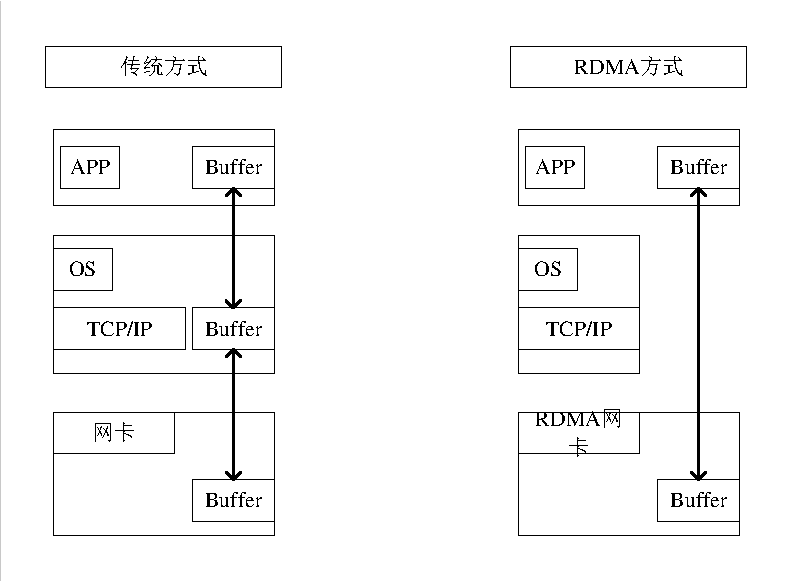
\includegraphics[width=\textwidth,keepaspectratio]{RDMA.pdf}
    \caption{RDMA 技术架构}
    \label{fig:RDMA}
\end{figure}

目前,有三种主要的 RDMA 网络协议: InfiniBand 、 RoCE (RDMA over Converged Ethernet) 和 iWARP (Internet Wide Area RDMA Protocol) 。 InfiniBand 技术发展最早也最完善,其他两种技术使用了与之相同的内核接口。 RoCE 是一种允许在以太网上执行 RDMA 的网络协议,它有两个版本: RoCEv1 直接建立在以太网链路层协议之上,而 RoCEv2 建立在 UDP 协议之上,与 IP 协议处于同等地位。 iWARP 协议更依赖于 TCP 协议并且只支持可靠通信,其性能有所下降。这三种协议都具有低延迟、高带宽和支持用户态协议栈的共同特点。使用了 RDMA 网络技术的用户态程序可以不通过内核就操纵专门的网卡将内存中的数据直接发送到远程机器的网卡中,同样直接将数据拷贝到内存。完全基于专用硬件的 RDMA 网络协议价格昂贵,由此诞生了两种基于它的新的 RDMA 技术: RoCE 和 iWARP ,它们的出现部分减少了对专用硬件的依赖,从而在硬件成本上部分提高了网络带宽。

 RDMA 技术具有显著的性能优势,主要体现在低延迟和高带宽两个方面。 RDMA 技术使得消息延迟非常低,在最新的硬件和服务器上,发送数十个字节大小的数据,其延迟只有几百纳秒。在以太网设备中,最高带宽会受限于以太网技术,其网速一般为 10~40Gb/s,而使用 RDMA 后,最高带宽可达 2.5~120GB/s。

\section{本章小结}

本章系统地介绍了Linux内存管理及相关技术的基础知识。首先,详细阐述了Linux物理内存管理机制,包括NUMA节点、内存区域、伙伴系统和页框管理等核心组件。其次,深入分析了Linux虚拟内存分页机制,重点介绍了多级页表结构及其工作原理。随后,探讨了CGroup V2在资源隔离和限制方面的创新设计。此外,本章还详细介绍了Linux内存回收机制,包括其调用栈和主要策略。最后,讨论了分层内存架构中的超越内存框架、非易失性内存技术以及RDMA技术,这些技术为现代内存管理提供了新的解决方案。本章内容为后续章节的研究奠定了理论基础,并为理解现代操作系统内存管理机制提供了全面的视角。
\chapter{面向异构后端的自适应主动卸载架构总体设计}

本章首先说明系统的设计,然后介绍介绍整体系统的架构、内核态和用户态的各个模块和组件,各个模块之间的交互,以及整个框架的执行流程。

\begin{figure}[h]
    \centering
    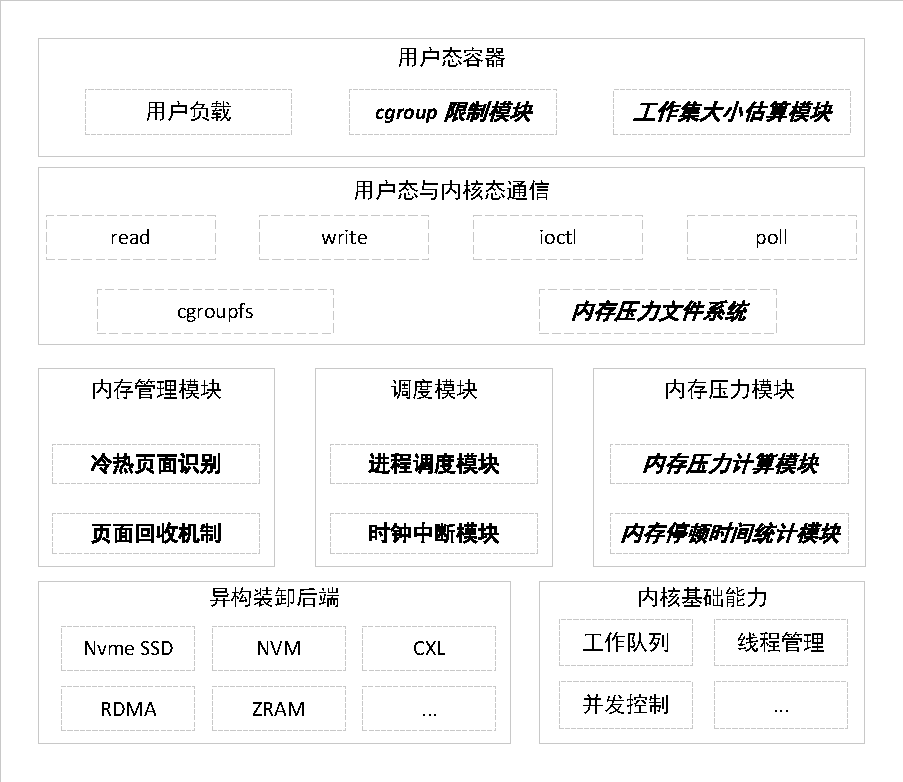
\includegraphics[width=\textwidth,keepaspectratio]{架构层次图.pdf}
    \caption{架构层次图}
    \label{fig:system_architecture_hierarchy}
\end{figure}

\section{需要分析与设计目标}

本方案旨在为异构后端提供一个基于内存压力的自适应透明卸载的框架,用户只需要基于异构卸载后端实现基于\texttt{Frontswap}接口,接入\texttt{swap}后端中,就可以实现冷内存的主动卸载。该框架具有显著的通用性和可扩展性,无需针对不同的用户负载特征和异构后端存储进行专门适配,
% 该系统采用了一种内核态-用户态协同方法,以实现对内存压力的感知和对容器工作集的动态优化。本研究将内存压力定义为由于内存资源不足而导致的应用程序性能下降,具体表现为同步内存回收操作所占用的时间片比例。基于此,我们首先在内核层构建了一个细粒度的内存压力模型,该模型能够实时、准确地反映系统的内存受限程度;基于该模型,我们在用户态设计了一种自适应的工作集估计算法,该算法能够根据内存压力动态调整容器的内存资源分配。

具体而言,本系统的设计目标涵盖以下功能性需求:
\begin{itemize}
\item 框架应具备自适应能力,能够适应不同用户负载特征和异构后端存储,无需进行专门适配
\item 框架应实现冷内存的透明卸载,且无需修改应用程序代码
\item 框架应确保用户负载的执行性能不受影响
\end{itemize}

在非功能性需求方面,主要包括以下要点:
\begin{itemize}
\item 框架应采用非侵入式设计,鉴于涉及内核操作,需充分考虑内核稳定性
\item 框架应尽可能降低自身开销,以避免对用户负载的执行性能产生负面影响
\end{itemize}

\section{系统架构}
本论文提出的面向异构后端的自适应主动卸载架构如图 \ref{fig:system_architecture_hierarchy} 所示。该架构采用内核态-用户态协同设计模式,旨在实现对容器内存压力的精确感知与主动卸载。图中加粗斜线表示新增模块,加粗部分表示修改模块。

框架底层由异构卸载后端和内核基础能力构成。异构卸载后端支持多种卸载后端,包括NVMe SSD、NVM、CXL、RDMA和ZRAM等,可通过实现Frontswap接口来接入swap以实现内存卸载。内核基础能力为框架运行提供必要支持,涵盖工作队列、线程管理及并发控制等核心功能。

框架的核心组件为内核态模块,由三个主要子模块构成:内存管理模块、调度模块和内存压力模块。内存管理模块包含冷热页面识别与页面分配功能,其中冷热页面识别与页面分配模块已进行优化改进;调度模块由进程调度与时钟中断模块组成,在每次调度时更新内存停顿时间统计模块中的累计时间;内存压力模块由内存压力计算与内存停顿时间统计模块组成,均为新增模块。

用户态容器包含三个核心模块:用户负载、CGroup限制模块及工作集大小估算模块。用户负载代表容器内运行的实际应用程序;CGroup限制模块基于Linux内核的CGroup机制,对容器内存资源使用进行约束;工作集大小估算模块根据内核态提供的内存压力信息,动态估算容器工作集大小,并据此调整CGroup内存限制,实现内存的主动卸载。

用户态与内核态之间通过多种通信机制实现交互。CGroupsfs用于和内核态的cgroup模块交互,获取和设置cgroup的内存限制。此外,通过自定义的mpfs接口获取内核态内存压力信息,并对容器内存资源配置进行动态调整。

\subsection{内存压力模块}

内存压力模块作为本架构的核心组件,承担着将内核检测到的内存短缺状况进行量化的关键任务,为用户态的工作集估计算法提供数据支撑,实现冷内存的主动卸载。该模块采用动态监测与分析机制,构建了多维度的内存压力评估模型,而非提供单一瞬时压力值。

内存压力模块的核心组件为内存停顿时间统计单元。该单元通过在内核同步内存回收路径上实施精细化插桩,捕获因内存分配请求无法立即满足而触发的同步回收事件。对于每个同步回收事件,系统在其开始和结束时更改状态,计算累计时间。在每次时钟中断和调度发生时,通过状态判断更新累计时间。

内存压力计算单元基于内存停顿时间统计单元提供的原始数据,采用加权平均、指数衰减等统计方法进行多维度分析。该单元不仅考虑最近一次停顿时间,还综合历史数据,生成能够平滑反映内存压力变化的量化指标。该指标设计旨在平衡响应速度与稳定性,既能够及时捕捉内存压力突变,又可避免因短期波动导致的误判,从而为用户态提供可靠的决策依据。

\subsection{通信模块}

通信模块负责实现内核态与用户态之间的高效数据交互,确保内存压力指标能够实时、准确地传递至用户态的容器管理组件。本模块基于proc虚拟文件系统实现,通过创建特定入口以标准文件I/O操作方式暴露内存压力信息。该入口采用百分比形式呈现内存压力指标,用户态程序可通过read系统调用直接获取相关信息。

为支持用户态程序对内存压力变化的实时响应,通信模块实现了poll系统调用接口。该接口采用事件驱动模型,允许用户态程序注册对特定文件描述符的事件监听。当内存压力指标超过预设阈值时,内核通过poll机制主动通知用户态程序,有效避免了频繁轮询带来的性能开销。这种事件驱动设计显著提升了用户态程序响应内存压力变化的及时性与效率。

\subsection{用户态容器}

用户态容器作为应用程序运行的隔离环境,是本架构实现内存压力感知与动态资源调整的执行单元。容器架构包含以下核心组件:

用户负载组件代表容器内运行的实际应用程序或服务。这些应用程序对底层的内存压力感知与资源调整机制保持透明,无需任何修改即可受益于架构提供的性能优化。

工作集大小估算模块是容器的关键组件,负责基于通信模块提供的内存压力信息,动态评估容器的当前工作集大小。

CGroup限制模块利用Linux内核的CGroup机制,对容器的内存资源使用实施动态约束。该模块通过与CGroupsfs文件系统交互,实时调整容器的软限制参数。工作集大小估算模块的输出作为CGroup限制模块的核心输入,指导其设置合理的内存限制,实现冷内存的主动卸载。

\subsection{内存管理模块}

内存管理模块作为Linux内核的核心组件,负责系统物理内存的分配、回收与管理。本框架主要修改了冷热页面识别机制和内存回收机制的较小部分。

冷热页面识别机制是内存回收和页面置换策略的基础。正确识别冷热页面才能在不损失性能的前提下,实现冷内存的主动卸载。本研究主要针对回收页面中匿名页和文件页的识别比例做了优化。

此外,为支持内存压力模块的统计需求,本框架在内存分配与回收的关键路径上实施了插桩,用于收集分配延迟、回收延迟等详细内存操作信息,为系统性能分析与优化提供了数据支撑。


\section{运行流程}

本节介绍系统运行流程,从框架初始化以及用户态和内核态的交互流程来介绍内存压力模块以及用户态容器组成的完整系统的典型流程,以进一步说明各个模块的之间的关系。

\subsection{框架初始化}

\begin{figure}[h]
    \centering
    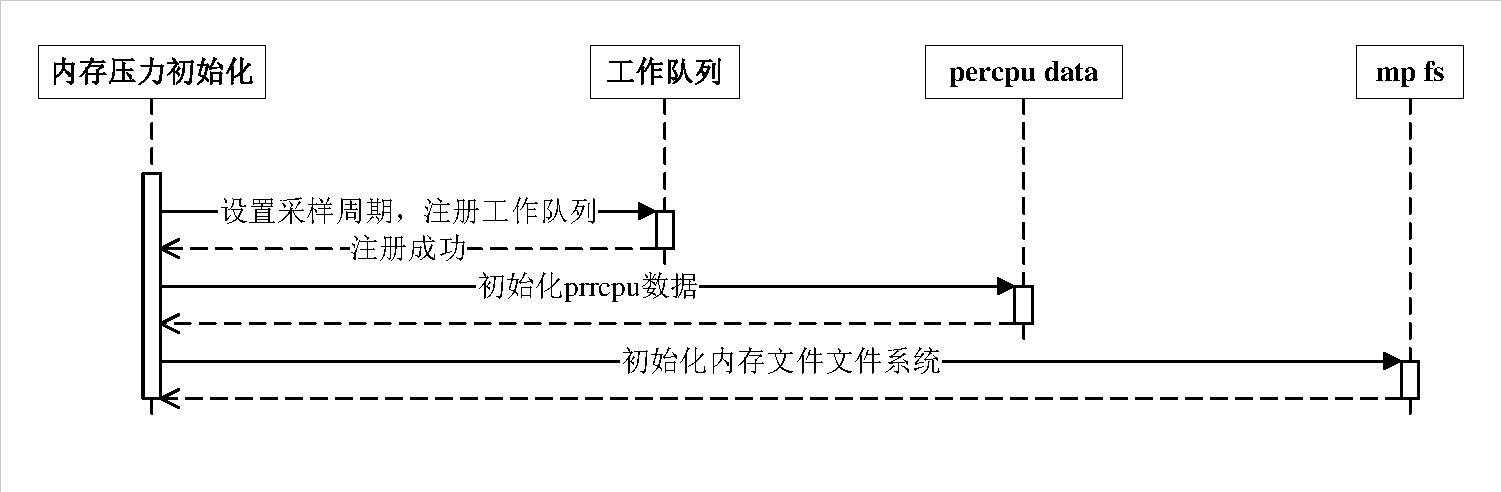
\includegraphics[width=\textwidth,keepaspectratio]{mp初始化.pdf}
    \caption{框架初始化}
    \label{fig:framework_initialization}
\end{figure}

本架构的初始化流程如图 \ref{fig:framework_initialization} 所示,主要包含三个关键阶段:

第一阶段完成采样周期与工作队列的配置。系统通过内核配置接口设定默认采样周期,并创建专用工作队列。采样周期直接影响内存压力监控的灵敏度,过长会错过瞬时尖峰,过短则增加性能开销。工作队列机制用于异步执行内存压力统计、计算及用户态报告等任务。

第二阶段初始化 per-CPU 变量。这些变量存储每个 CPU 核心的内存压力统计信息,包括停顿累计时间、非空先时间等信息。

第三阶段初始化并挂载 mpfs 文件系统。该虚拟文件系统通过内核 mount 调用挂载于指定目录,并与 VFS 层集成。mpfs 通过标准文件操作将内存压力信息暴露给用户态,使应用程序能够实时监控和响应系统内存状态。

\subsection{面向异构后端的自适应主动卸载框架的执行流程}
\label{sec:面向异构后端的自适应主动卸载框架的执行流程}




\begin{figure}[h]
\centering
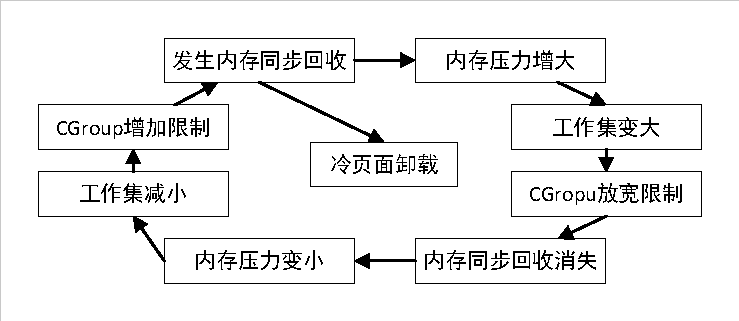
\includegraphics[width=\textwidth,keepaspectratio]{负反馈.pdf}
\caption{负反馈闭环执行流程}
\label{fig:feedback_loop}
\end{figure}

\begin{figure}[h]
\centering
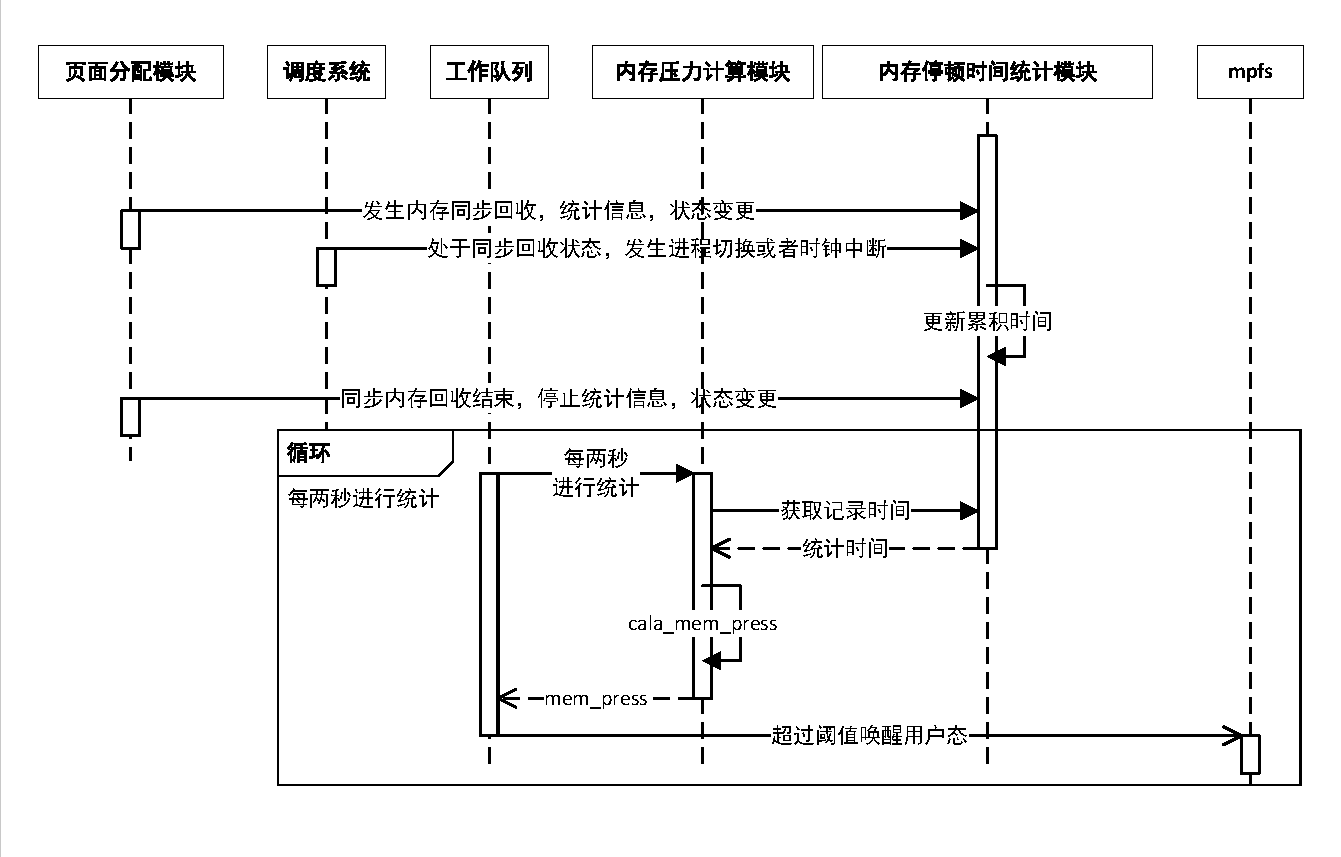
\includegraphics[width=\textwidth,keepaspectratio]{序列图1.pdf}
\caption{执行流程1}
\label{fig:kernel_sequence_diagram_1}
\end{figure}

\begin{figure}[h]
\centering
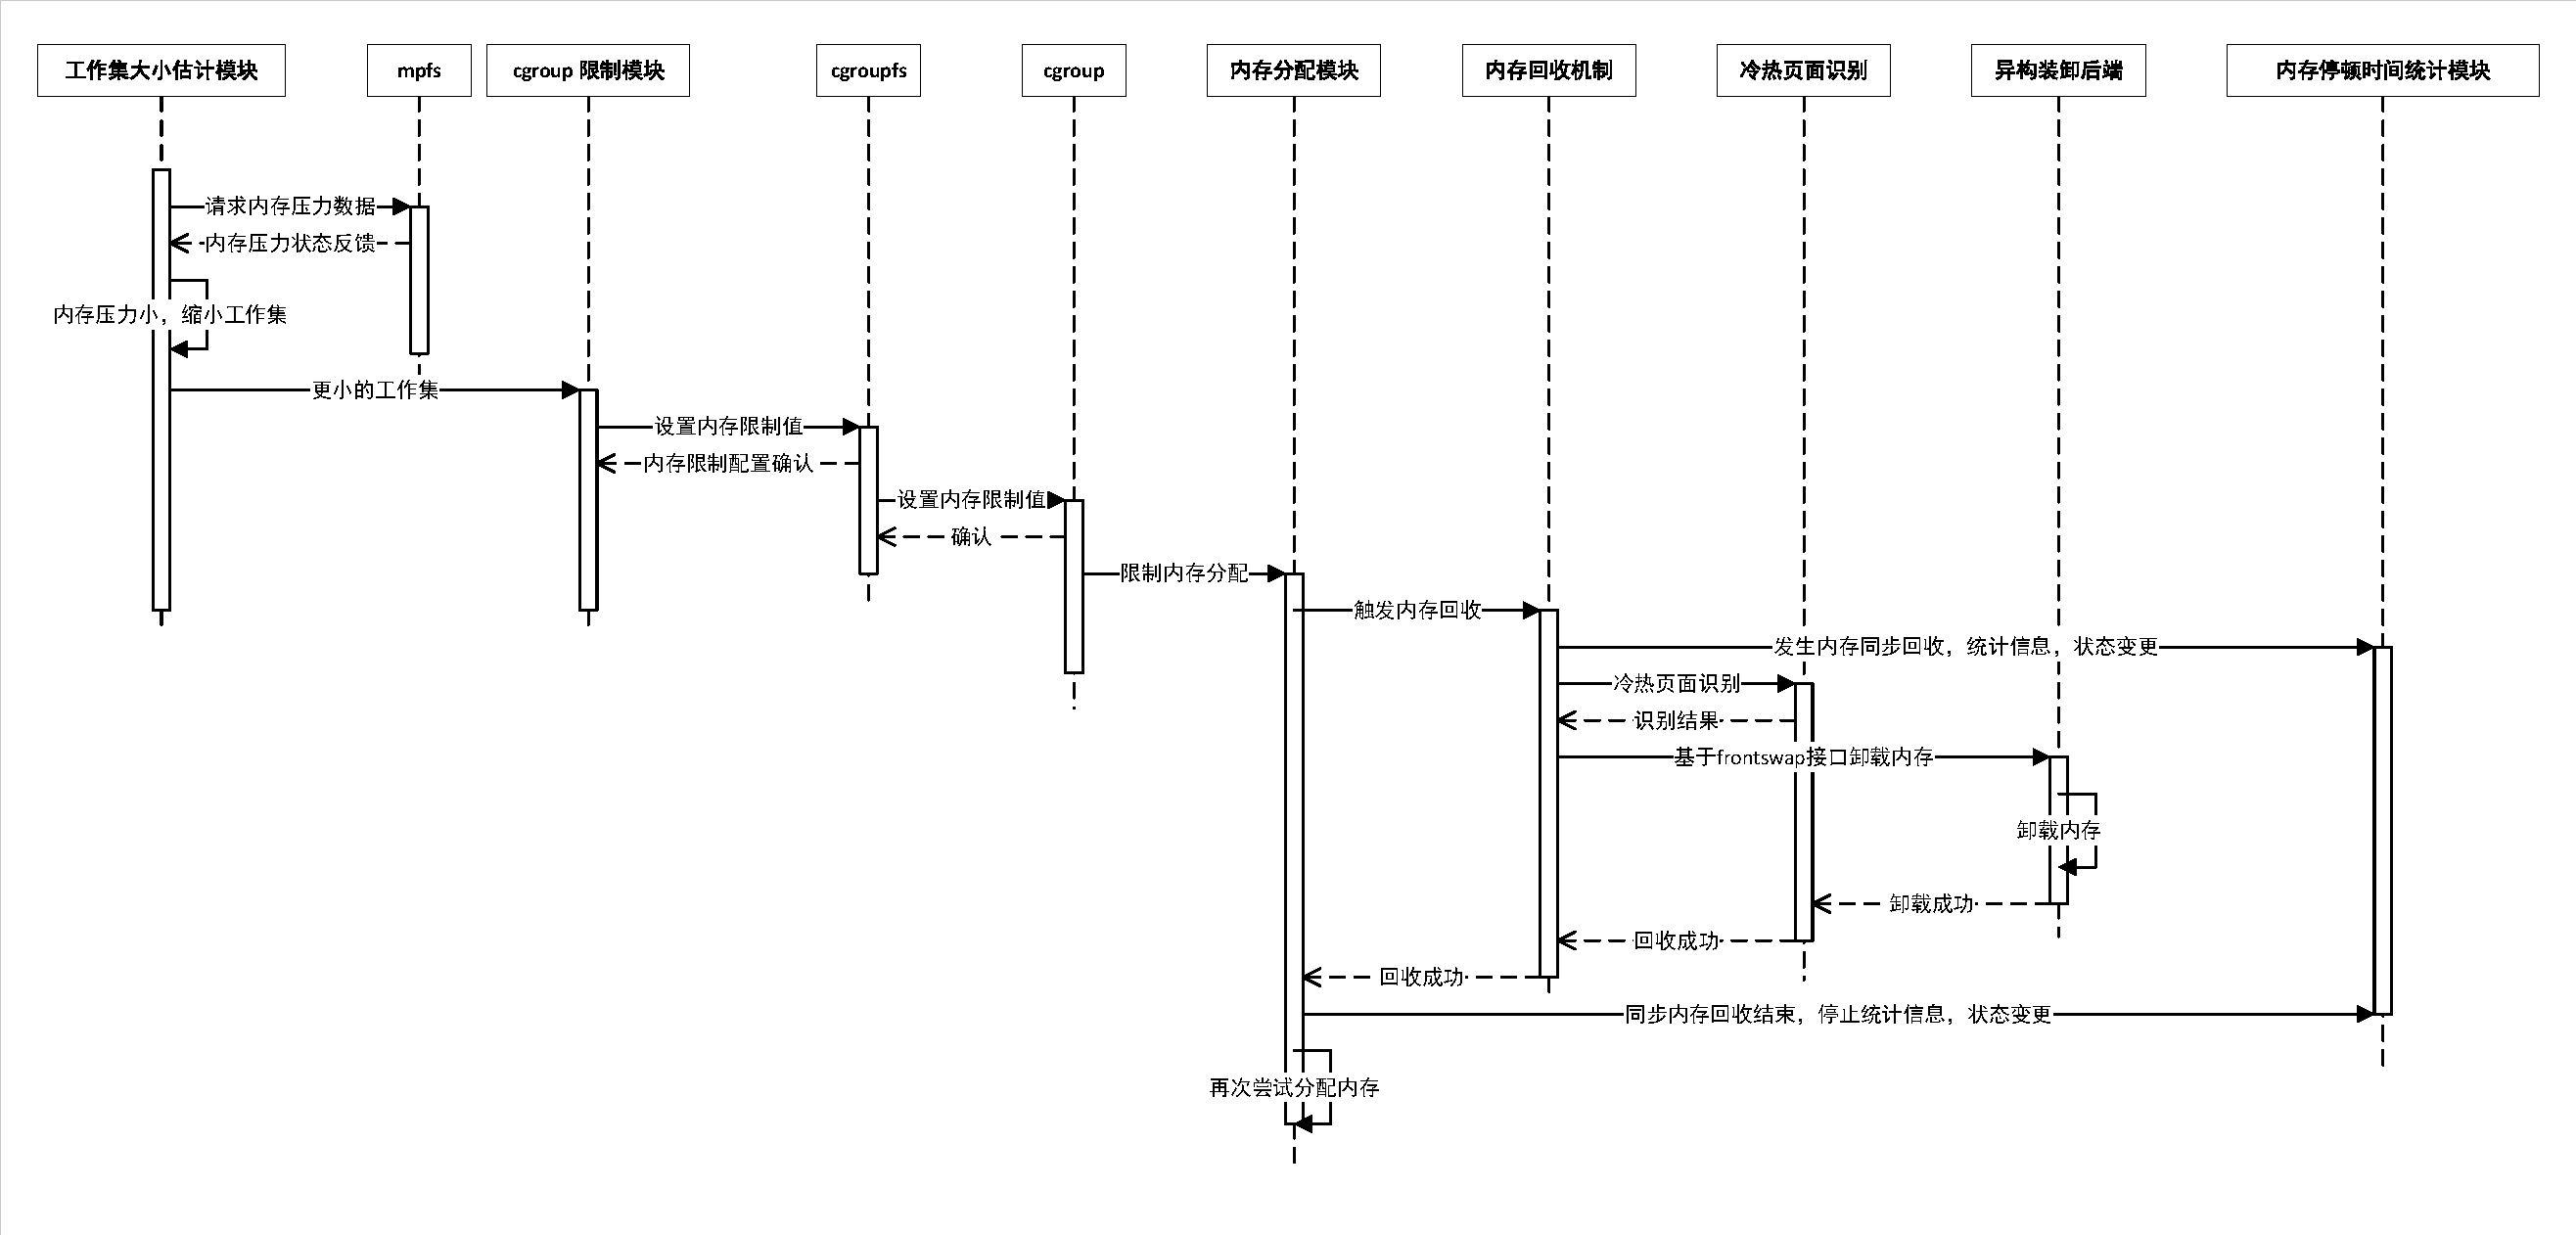
\includegraphics[width=\textwidth,keepaspectratio]{序列图2.pdf}
\caption{执行流程2}
\label{fig:kernel_sequence_diagram_2}
\end{figure}

\begin{figure}[h]
\centering
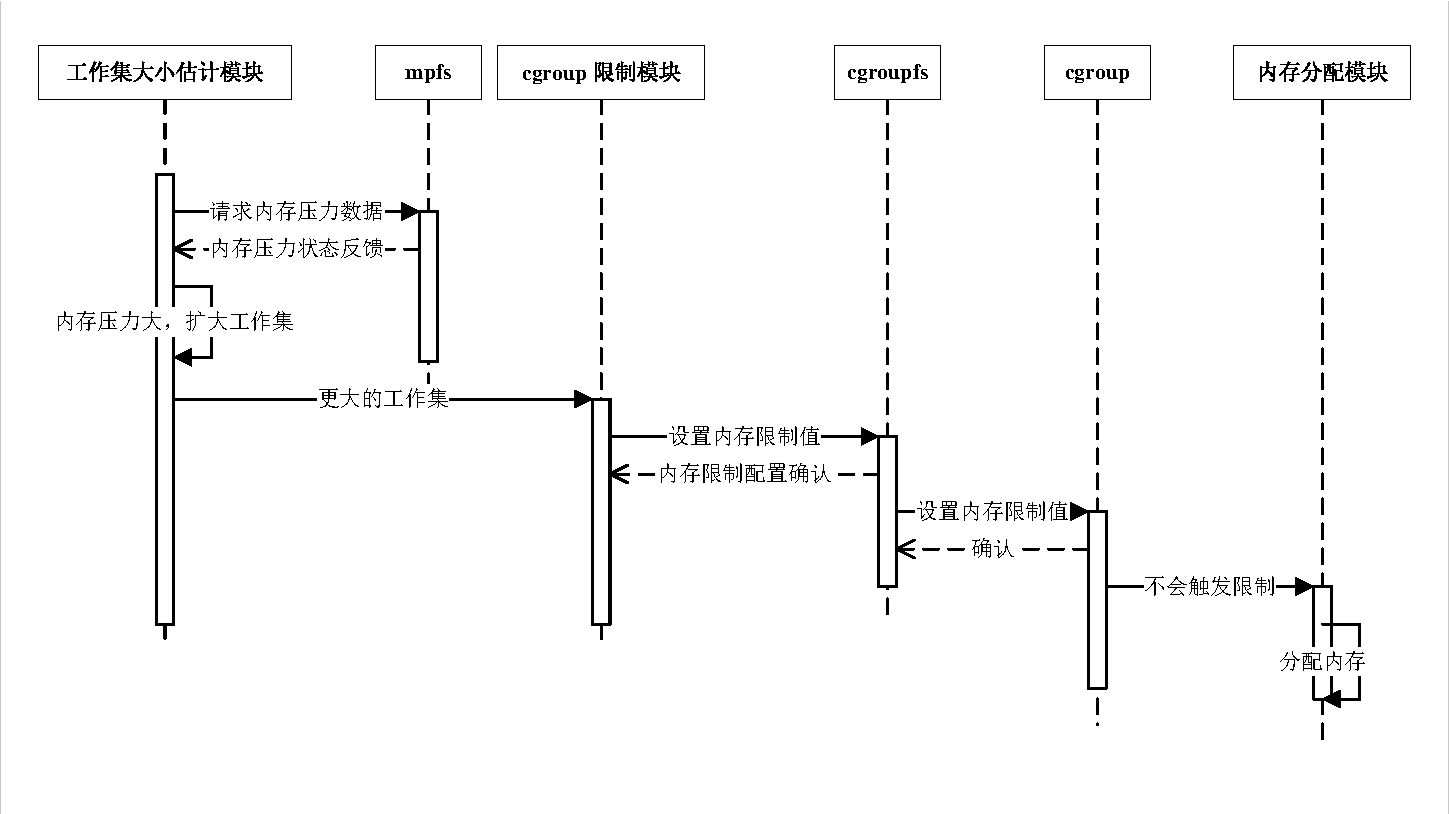
\includegraphics[width=\textwidth,keepaspectratio]{序列图3.pdf}
\caption{执行流程3}
\label{fig:kernel_sequence_diagram_3}
\end{figure}

本节详细阐述了框架主动卸载冷内存的机制。该框架通过动态调整工作集大小来响应内存压力变化,工作集大小的调整又反作用于内存压力。在此过程中,冷页面被卸载到异构后端,实现冷内存的主动卸载。整个负反馈过程如图 \ref{fig:feedback_loop} 所示。

基于图 \ref{fig:kernel_sequence_diagram_1}、图 \ref{fig:kernel_sequence_diagram_2} 和图 \ref{fig:kernel_sequence_diagram_3},本研究详细阐述了面向异构后端的自适应主动卸载框架的执行流程及各模块间的交互机制:

\textbf{阶段一:内存压力监测}
图 \ref{fig:kernel_sequence_diagram_1} 展示了内存压力监测阶段。该阶段始于内存分配请求的发起。当系统无法立即满足应用程序的内存请求时,触发内存同步回收机制。内存停顿时间统计模块介入,记录系统状态并启动回收过程的持续跟踪。在回收过程中,系统发生进程切换或时钟中断时,检查状态并更新累计时间,为后续内存压力分析提供数据支持。同步回收结束时,统计模块停止记录并完成状态变更。内存压力计算模块以固定时间间隔(本系统设置为每两秒)进行一次周期性统计,采用加权平均、滑动窗口等统计方法处理原始数据,生成量化的内存压力指标。若注册了poll且超过阈值,则唤醒用户态。

\textbf{阶段二:内存压力小,工作集调整与冷页卸载}
图 \ref{fig:kernel_sequence_diagram_2} 展示了内存压力较小时的处理流程。用户态的工作集大小估计模块通过 mpfs 接口发起内存压力数据请求,通常为阻塞式读取操作。内核态的内存压力模块通过 mpfs 接口反馈最新内存压力状态后,工作集大小估计模块运行特定估计算法。若内存压力较小,则计算出更小的工作集。通过 CGroup 限制模块,将内存限制传递给内核中的 CGroup 机制。CGroup 机制限制内存分配模块,在后续内存分配时触发内存回收,进而激活内核的内存回收机制,进入内存停顿时间统计模块,开始统计信息并变更状态。同时启动冷热页面识别过程,区分内存中的热页和冷页。冷热页面识别模块完成页面属性识别后,将识别结果告知内存回收机制。系统根据识别结果,利用 frontswap 接口将冷页从物理内存卸载到预先配置的异构后端中。当冷页成功卸载后,frontswap 接口向内存回收机制发送卸载成功的反馈信息,停止统计信息并变更状态。

\textbf{阶段三:内存压力大,内存回收与卸载}
图 \ref{fig:kernel_sequence_diagram_3} 展示了内存压力较大时的处理流程。由于发生了同步回收,内存压力增大,工作集大小估计模块计算出更大的工作集,并通过 CGroupfs 调整内存限制。若无内存限制,则不会触发同步回收,内存压力减小后返回第二阶段。

\section{本章小结}

\begin{figure}[h]
    \centering
    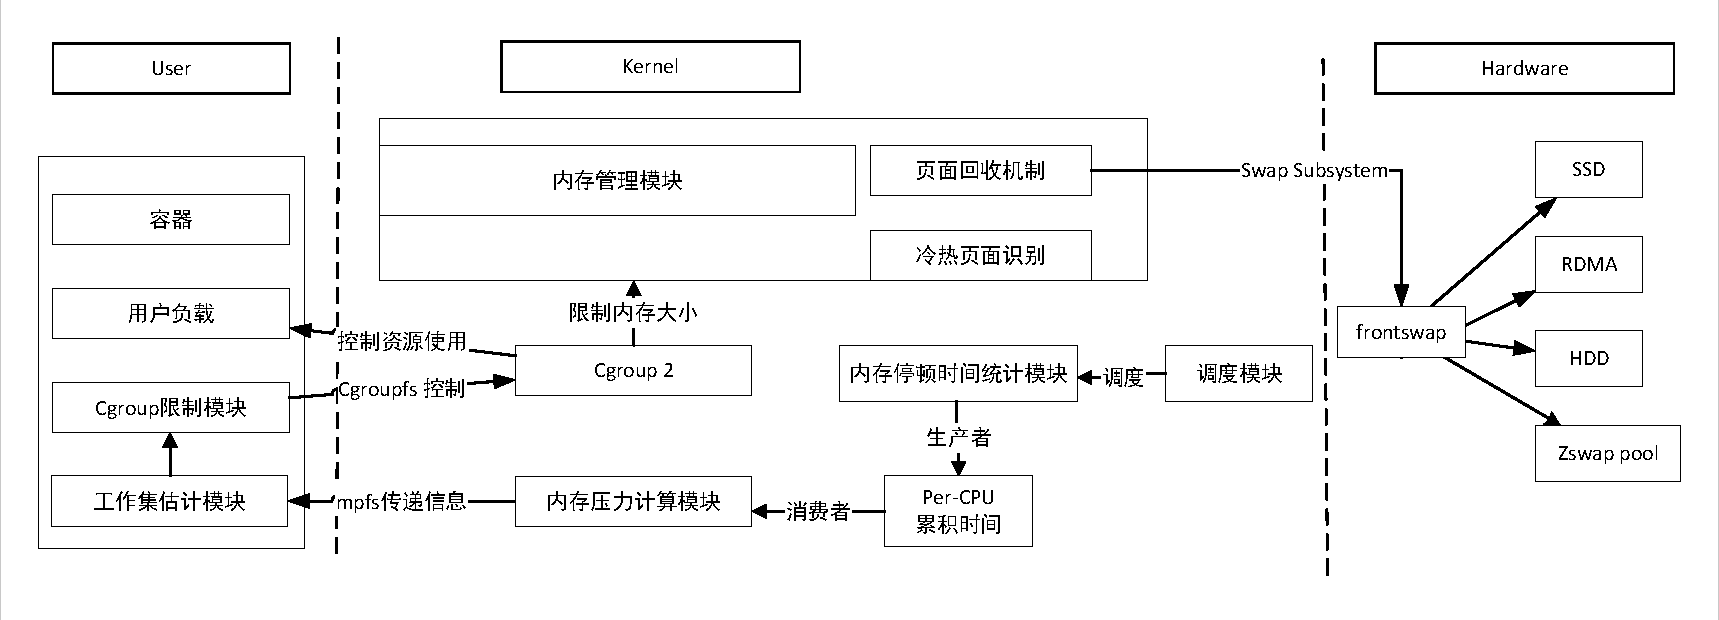
\includegraphics[width=\textwidth,keepaspectratio]{架构图.pdf}
    \caption{系统整体架构}
    \label{fig:system_architecture}
\end{figure}

本章阐述了面向异构后端的自适应主动卸载框架的整体架构及其关键模块,详细介绍了框架初始化流程以及用户态与内核态协同的异构内存资源动态管理机制。系统架构如图 \ref{fig:system_architecture} 所示。

在用户空间层面,系统部署了工作集估算器和 CGroup 管理器两个核心组件。工作集估算器通过mpfs 持续获取内核态的内存压力信息,并支持基于事件的通知机制以提升响应时效性。CGroup 管理器负责执行工作集估算器的决策,通过调整 CGroup V2 内存限制参数实现对容器内存资源的动态调控。

内核空间的核心组件为内存压力监控器,该组件深度嵌入内核内存管理子系统。内存压力监控器采用静态插桩技术,在同步内存回收时记录中断时间片,并与调度系统交互计算回收延迟,生成量化压力信号。该信号通过 mpfs 文件系统周期性暴露给用户空间,同时实现基于事件的通知机制,当内存压力超过预设阈值时主动通知工作集估算器。

系统采用负反馈调节机制实现内存资源的精细化管理。当内存压力较低时,工作集估算器指示 cgroup 管理器收缩容器内存分配上限,主动触发内核页面回收机制,将不活跃页面换出到分层存储,实现"预先释放,主动应对"策略。当内存压力升高时,内存压力监控器迅速检测并更新压力信号,工作集估算器触发负反馈调节,重新评估容器内存需求,计算更大工作集大小,CGroup 管理器通过调整 memory.high 等参数放宽容器内存使用限制,减少缺页中断,保障应用性能。

该机制形成了完整的负反馈闭环:内存压力监控器提供实时压力反馈,工作集估算器进行决策,cgroup 管理器执行资源控制,容器工作负载在调整后的资源约束下运行,其内存访问行为进一步影响内核内存压力,实现持续的自适应动态调节。这种协同机制使系统能够灵敏、准确地响应内存压力变化,在保证关键应用性能的同时最大化异构内存系统利用率,有效避免内存过度分配导致的系统抖动和性能下降。
\chapter{基于同步内存回收的内存压力量化算法的设计与实现}
\label{chap:基于同步内存回收的内存压力量化算法的设计与实现}
本章详细介绍了基于同步内存回收延迟的内存压力量化算法的设计与实现细节。首先分析了同步回收延迟与内存压力的关联性,然后提出了基于同步回收延迟的内存压力量化算法的设计思想,关键技术细节,最后介绍了该算法的实现细节。

\section{同步内存回收延迟与内存压力的关联性建模}

在内存管理研究中,工作集估计算法作为核心组件,其精确性直接影响内存分配策略与页面置换决策的效能。如\ref{sec:工作集估计算法研究历史与现状}节所述,现有工作集估计方法可归纳为三类典型范式:基于统计采样的近似计算模型、依托系统运行时特征的启发式预测算法,以及基于机器学习模型的离线训练-在线预测框架。然而,机器学习算法在面对新型应用场景时存在泛化能力不足的问题,其预测性能有待进一步验证。

基于统计特征的启发式算法在内存管理领域被广泛应用,原因在于它们能够实时适应系统运行状态的变化,满足动态内存管理的需求。在这类算法中,内存压力指标是一个核心概念,它量化了系统内存资源的紧张程度,为内存卸载决策提供了重要依据。现有研究通常采用缺页中断频率、页面分配速率等多种统计指标来表征内存压力,并通过这些指标来估计工作集大小。然而,这些传统方法存在两个关键缺陷:

\begin{itemize}
    \item 内存压力指标与工作集大小的函数关系呈现显著的非线性特征。例如,工作集转换可能导致大量缺页中断,从而干扰算法对工作集大小的准确判断。
    \item 内存压力指标未充分考虑异构存储设备在性能上的显著差异。以机械硬盘与NVM为例,二者可能发生相同次数的缺页中断,但其处理压力存在显著差异。由于NVM能够快速处理缺页中断,在不影响性能的前提下,可适当缩小工作集以节约内存资源。
\end{itemize}

本研究基于Linux内核同步内存回收机制提出新型压力度量指标,其数学表征为:
\begin{equation}
    \label{eq:mem_pressure}
    mem\_pressure = \frac{T_{sync}}{T_{epoch}}
\end{equation}

其中\(T_{sync}\)表示同步回收累积耗时,\(T_{epoch}\)为监控时间窗口。\(T_{sync}\)可通过在Linux内核的 \_\_alloc\_pages\_direct\_reclaim 函数入口和出口处插桩,记录每次同步回收操作的开始和结束时间戳,并在时间窗口内对所有回收操作的持续时间进行累加得到。\(T_{epoch}\) 表示一个完整的监控时间窗口,通常设置为系统的采样周期,例如2秒。 mem\_pressure  的取值范围为 [0, 1],对应百分比表示为0\%\~{}100\%。当  mem\_pressure  接近0时,表示系统几乎没有内存压力:当其接近1时,表示系统几乎所有时间都在进行同步内存回收,此时系统处于严重的内存压力状态,性能将显著下降。

该内存压力指标的提出基于以下理论分析:

\begin{enumerate}
    \item 当系统内存充足时,同步回收操作极少发生,$T_{sync}$ 接近于零;
    \item 当内存压力逐渐增加时,$T_{sync}$ 呈现出与压力程度近似线性的增长;
    \item 对于异构存储后端,高性能设备(如NVM)处理同等数量的缺页中断所需时间更短,计算得到的内存压力值也相应较低,准确反映了实际系统状态。
\end{enumerate}

该方法直接测量因内存压力导致的性能损失时间,而非间接指标。同步内存回收发生时,应用程序必然被阻塞,这部分时间的占比直接反映了应用因内存不足而遭受的性能损失,建立了内存压力与性能影响之间的直接联系。

在异构卸载环境中,该方法能够自动适应不同存储后端的性能特性。对于高性能存储设备(如NVM或Optane),即使发生相同次数的缺页中断,由于其处理速度更快,测得的同步回收时间会相应减少,从而体现出较低的内存压力值;而对于传统机械硬盘,相同次数的缺页中断会导致更长的回收时间,反映出更高的性能损失和内存压力。这种适应性消除了传统方法中需要为不同存储设备单独调整评估参数的复杂性。

无论应用程序是内存密集型、计算密集型还是I/O密集型,当内存不足导致性能下降时,都会表现为同步回收时间的增加。这使得该方法能够在不同类型的工作负载下保持一致的评估标准,无需针对特定应用类型进行定制化调整。

基于上述理论分析,下一节将详细介绍如何设计和实现基于同步内存回收延迟的内存压力量化算法,包括多核系统中的加权聚合策略、指数移动平均平滑处理以及定点数优化技术。

\section{基于同步内存回收延迟的内存压力量化算法}
\label{sec:基于同步内存回收延迟的内存压力量化算法}

在 \ref{sec:Linux内存回收机制} 节中,已经对 Linux 内核同步内存回收机制做了详细的分析,分析表明,函数 \_\_alloc\_pages\_direct\_reclaim 的执行时间是反映同步回收延迟的重要指标。基于此本节提出了一种内存压力检测方法。该方法利用内核插桩技术,在 \_\_alloc\_pages\_direct\_reclaim 函数的入口和出口处改变状态,然后在内核中每次发生同步中断的时候去更新累计时间和CPU的非空闲时间,从而直接获取每次同步回收操作的耗时。为了综合反映多  CPU  系统中不同核心的负载差异,本研究引入了多  CPU  加权聚合策略。此外,为了平滑压力数据、减少短期波动的影响,本研究采用了指数移动平均算法。此外,还采用了定点数优化技术,显著提高了计算效率。

\subsection{多核加权聚合}
\label{sec:weighted_aggregation}
本研究通过插桩技术得到的是各处理器核心在同步内存回收过程中的阻塞时间 \(T_c^{block}\),其中 \(c\) 表示核心编号,需要将多个核心的 \(T_c^{block}\) 聚合为一个压力值。然而,采用简单的算术平均方法计算系统压力:
\begin{equation}
    \label{eq:simple_average_pressure}
    Pressure_{simple} = \frac{\sum_{c=1}^{n} T_c^{block}}{\Delta T \times n} \times 100\%
\end{equation}

其中,\(\Delta T\) 为采样周期,\(n\) 为处理器核心数量,简单平均算法在多核系统中存在两个关键理论缺陷,影响其准确表征系统内存压力的能力。

首先,简单平均算法忽略了处理器核心间负载分布的不均衡性,导致所谓的"空闲核心稀释效应"(idle core dilution effect)。在异构负载环境中,当少数核心承担主要计算任务而其他核心相对空闲时,高负载核心所反映的内存压力信号会被空闲核心的数据稀释。以四核系统为例,若其中一个高负载核心记录了0.5秒的同步回收阻塞时间,一个轻负载核心记录了0.1秒,而其余两个核心几乎无阻塞(均为0秒),则系统压力计算结果为:
\[
Pressure_{simple} = \frac{0.5 + 0.1 + 0 + 0}{1.0 \times 4} \times 100\% = 15\%
\]

此结果明显低估了系统实际承受的内存压力,因为对于执行关键任务的处理器核心而言,50\%的时间(0.5秒/1.0秒)被阻塞在内存回收操作上,这种严重的资源受限状态在平均计算中被显著弱化。

其次,简单平均算法对所有核心赋予等价权重,未能反映不同核心在系统整体性能中的贡献差异。在工作负载不均衡的场景下,主要完成计算任务的核心对系统性能的影响更为显著。考虑一个双核系统,\(\Delta T\) 为100ms。核心0处于高负载状态,非空闲时间为90ms(占总时间的90\%用于处理任务),其中60ms用于同步内存回收,30ms用于处理其他任务;而核心1基本处于轻负载状态,非空闲时间仅20ms(占总时间的20\%),其中10ms用于同步内存回收,10ms用于处理其他任务。简单平均算法计算得出的系统压力为:
\[
Pressure_{simple} = \frac{60 + 10}{100 \times 2} \times 100\% = 35\%
\]

这一结果未能反映核心0作为主要计算资源的压力状态,从而可能导致资源管理决策的偏差。

为克服上述缺陷,本研究提出采用加权聚合算法,这种启发式方法借鉴了多领域中的贡献度加权思想\citing{Hwang1981MultipleAD}。类似的权重分配策略在计算机体系结构中的不对称多处理器调度\citing{petrucci2012lucky}中得到了广泛应用。该算法的核心思想是:根据每个处理器核心的运行时间分配权重。核心的运行时间越长,表明其在采样周期内处理的任务越多,其上发生的同步内存回收事件对系统整体性能的影响也越显著,其行为也更具有代表性。加权聚合算法的计算公式如下:

\begin{equation}
    \label{eq:weighted_aggregation}
    Pressure_{weighted} = \frac{\sum_{c=1}^{n} (T_c^{block} \times W_c)}{\sum_{c=1}^{n} W_c} \times 100\%
\end{equation}

其中,\(T_c^{block}\) 表示核心 \(c\) 在采样周期 \(\Delta T\) 内的同步内存回收总延迟时间,\(W_c\) 表示核心 \(c\) 的权重,即其在采样周期 \(\Delta T\) 内的非空闲时间,非空闲时间直接反映了该核心的有效工作量。分母中的 \(\sum_{c=1}^{n} W_c\) 表示所有核心的非空闲时间总和。通过这种加权方式,算法能够有效降低或消除空闲核心的噪声影响,同时更准确地反映不同核心负载对系统整体性能压力的贡献,从而提供更可靠、更具代表性的内存压力评估结果。应用加权算法于前述双核系统示例,其结果为:
\[
Pressure_{weighted} = \frac{60 \times 90 + 10 \times 20}{90 + 20} \times 100\% = 51\%
\]

表\ref{tab:weighted_vs_simple}直观展示了简单平均与加权聚合算法在三种典型负载场景下的表现差异。可以看出,随着核心负载分布不均衡程度的增加,两种算法计算结果的差异也越显著,尤其在高度不均场景下,简单平均算法严重低估了系统实际内存压力。

\begin{table}[htbp]
    \centering
    \caption{简单平均与加权聚合算法在不同核心负载条件下的比较}
    \label{tab:weighted_vs_simple}
    \begin{tabular}{lccc}
        \toprule
        \multirow{2}{*}{\textbf{负载场景}} & \multicolumn{2}{c}{\textbf{每核心数据}} & \multirow{2}{*}{\textbf{系统压力计算结果}} \\
        \cmidrule(lr){2-3}
         & \textbf{阻塞时间 $T_c^{block}$ (ms)} & \textbf{非空闲时间 $W_c$ (ms)} & \\
        \midrule
        \multirow{4}{*}{均匀负载} & 核心0: 400 & 核心0: 800 & 简单平均: 50\% \\
         & 核心1: 400 & 核心1: 800 & 加权聚合: 50\% \\
         & 核心2: 400 & 核心2: 800 & (两种方法结果相同) \\
         & 核心3: 400 & 核心3: 800 & \\
        \midrule
        \multirow{4}{*}{中度不均} & 核心0: 600 & 核心0: 900 & 简单平均: 40\% \\
         & 核心1: 400 & 核心1: 700 & 加权聚合: 47\% \\
         & 核心2: 300 & 核心2: 500 & (加权方法更准确) \\
         & 核心3: 100 & 核心3: 100 & \\
        \midrule
        \multirow{4}{*}{高度不均} & 核心0: 800 & 核心0: 950 & 简单平均: 27.5\% \\
         & 核心1: 300 & 核心1: 500 & 加权聚合: 63\% \\
         & 核心2: 0 & 核心2: 50 & (简单平均严重低估) \\
         & 核心3: 0 & 核心3: 0 & \\
        \bottomrule
    \end{tabular}
\end{table}


\subsection{指数移动平均算法}
\label{sec:exponential_smoothing}
在获取基于处理器核心的非空闲时间加权的内存压力指标后,本研究进一步考虑压力数据的平滑性以及长期趋势的分析。原始的压力数据(无论是简单平均还是加权平均)可能会因为短暂的、偶然的事件而产生剧烈波动,这些波动可能会掩盖真实的压力趋势。因此,需要采用一种有效的方法对压力数据进行平滑处理,以减少短期波动的影响,同时保留长期趋势信息。指数移动平均(Exponential Moving Average, EMA)算法\citing{gardner1985exponential}在多个方面优于传统平滑方法:首先,相较于简单移动平均(SMA),EMA能更快地响应压力变化;其次,与加权移动平均(WMA)相比,EMA的计算效率更高且内存占用更小;最后,相比于Kalman滤波等复杂算法,EMA具有参数调整简单、计算开销低等优势,特别适合资源受限的实时操作系统环境。


EMA 算法的核心思想是对新旧数据进行加权平均,但与简单算术平均赋予所有数据相同权重不同,EMA 赋予旧数据的影响随时间推移呈指数衰减。这种处理方式更符合实际系统的运行特征:最近发生的事件对当前系统状态的影响通常更大,而较早发生的事件的影响则逐渐减弱。具体来说,EMA 的计算公式为:
\begin{equation}
    EMA_{new} = EMA_{old} \times \alpha + P_{current} \times (1 - \alpha)
    \label{eq:EMA}
\end{equation}

其中,\(EMA_{new}\) 和 \(EMA_{old}\) 分别代表当前时刻和上一时刻的 EMA 值,\(P_{current}\) 是当前时刻的压力值,\(\alpha\) 是一个介于 0 和 1 之间的衰减因子(也称平滑因子)。衰减因子 \(\alpha\) 的数值范围具有明确的物理意义:当 \(\alpha\) 接近 1 时,系统对历史数据的依赖性较高,对新数据的敏感度较低,产生的平滑曲线更加稳定但响应滞后;当 \(\alpha\) 接近 0 时,系统对当前数据的重视度高,对历史数据影响较小,平滑曲线能够快速响应压力变化但可能保留更多短期波动。衰减因子 \(\alpha\) 决定了旧数据影响力衰减的速度,也即决定了 EMA 对历史数据的记忆长度。为了便于参数设置,本文将 \(\alpha\) 与系统可观测参数关联,定义计算关系式为:
\begin{equation}
\alpha = e^{-\Delta T / \tau}
\label{eq:alpha}
\end{equation}

其中,\(\Delta T\) 是采集内存压力数据的周期(例如,每2秒采样一次),\(\tau\) 则反映了希望EMA追踪的压力趋势的时间尺度(例如,10秒、60秒或300秒)。根据公式(\ref{eq:alpha}),当 \(\tau\) 越大时,\(\alpha\) 越接近1,EMA曲线越平滑,对短期波动的抑制能力越强,但对真实压力变化的反应也越迟钝;反之,当 \(\tau\) 越小时,\(\alpha\) 越接近0,EMA曲线对新数据的响应越灵敏,但平滑效果也越差。

相比于简单平均或固定窗口的移动平均算法,EMA 算法具有显著优势。首先,EMA 算法的计算非常高效。它仅需存储上一时刻的 EMA 值,无需维护一个包含大量历史数据的窗口,计算复杂度为 \(O(1)\)。这使得 EMA 非常适合于资源受限的嵌入式系统或需要高频采样的实时监控系统。其次,EMA 算法的参数可调性提供了极大的灵活性。通过调整衰减因子(即调整时间窗口),可以在快速响应和数据平滑之间找到最佳平衡点。这使得 EMA 能够适应不同的应用场景和性能需求。最后,也是最重要的一点,EMA 算法能够有效地追踪压力数据的长期趋势。它不仅能平滑短期波动,还能清晰地展现压力随时间变化的整体走向,帮助及时发现潜在的性能瓶颈或系统异常。

在整个内存压力监控框架中,EMA算法作为时间维度的数据处理层,接收来自多核加权聚合处理后的压力数据,进一步消除时间维度的噪声干扰,为系统提供稳定的内存压力趋势信息,最终用于指导内存管理决策。

\subsection{时间校准与数据处理优化机制}
\label{sec:time_calibration_and_data_processing}
在高并发环境中,内存压力的精确测量面临调度延迟和数据积压等挑战,可能导致采样周期偏移和统计指标失真。本节从时间校准和数据处理两个维度展开分析,提出了相应的优化机制,确保内存压力量化的准确性和稳定性。

\subsubsection{周期性任务的时间校准}

设理想的任务执行时间序列为等间隔离散点:
\[
t_0, \quad t_0 + T, \quad t_0 + 2T, \quad t_0 + 3T, \quad \dots
\]
其中\(T\)为系统设定的基准周期。然而,受系统负载和调度策略影响,实际执行时刻常呈现非线性偏移:
\[
t_0, \quad t_0 + T + \Delta_1, \quad t_0 + 2T + \sum_{i=1}^2\Delta_i, \quad \dots
\]
其中\(\Delta_i \in \mathbb{R}^+\)表示第\(i\)周期的累积延迟。

这种时间偏移若不加处理,会导致采样间隔不均,影响内存压力的准确评估。为解决此问题,本研究设计了基于相位同步的时间校准算法。该算法通过定义两个关键参数实现:
\begin{align}
    \text{missed\_periods} &= \left\lfloor \frac{\text{now} - \text{expires}}{T} \right\rfloor
    \label{eq:missed_periods} \\
    \text{next\_execution} &= \text{expires} + (\text{missed\_periods} + 1) \times T
    \label{eq:next_execution}
\end{align}

式中,\(\text{now}\)表示当前系统时间戳,\(\text{expires}\)表示上次任务完成时刻。算法首先通过公式\ref{eq:missed_periods}计算当前已错过的完整周期数,然后利用公式\ref{eq:next_execution}确定下次执行时刻,将其映射至最近的理想时间点。这种方法不仅修正了当前周期的偏移,更重要的是通过全局时间重映射,有效抑制了时序偏移的级联传播,确保长期运行时的稳定性。

\subsubsection{积压数据的处理机制}

在内存压力监测过程中,生产者(同步回收监测)和消费者(压力计算)之间的速率不匹配可能导致数据积压,进而引发统计指标异常。针对这一问题,本研究提出了两种互补的处理机制:

\paragraph{截断补偿机制} \quad 在无锁采样环境下,时间记录机制存在固有的竞态条件,可能导致某一周期内记录的时间增量溢出至下一周期。特别是在系统承受持续高压力时,单个周期内累积的时间样本可能超过周期本身的长度,产生超过100\%的非物理压力值。

设当前采样周期长度为\(\textit{period}\),对于任一周期内检测到的累积同步回收时间\(v\),当\(v > \textit{period}\)时,系统执行如下处理:
\begin{equation}
v_{\text{current}} = \min(v, \textit{period}), \quad v_{\text{carryover}} = v - v_{\text{current}}
\end{equation}
其中,\(v_{\text{current}}\)表示当前周期内实际统计的有效累积时间,\(v_{\text{carryover}}\)表示超出阈值的剩余时间,将被递延至下一统计周期处理。

该机制基于以下理论保证:
\begin{enumerate}
    \item \textbf{总量守恒原理}:截断补偿确保所有记录的时间增量都被计入统计,满足任意连续\(n\)个周期的累积等式:
    \begin{equation}
        \sum_{k=1}^n v_{\text{current}}^{(k)} \equiv \sum_{k=1}^n v^{(k)}
    \end{equation}
    \item \textbf{误差非累积性}:当时间增量从周期\(P\)溢出至周期\(P+1\)时,根据时间守恒原理,它必然在周期\(P\)中释放了等量的时间,使得误差不会随时间累积。
    \item \textbf{时间序列同态性}:该机制对原始压力曲线进行了时间保持型变换,延迟报告但不改变曲线的积分特性,确保长期评估的准确性。
\end{enumerate}

\paragraph{指数加速收敛} \quad 当系统连续多个周期未能进行数据更新时,标准的指数移动平均(EMA)算法需要进行适应性调整。回顾公式\ref{eq:EMA}中的标准EMA更新公式:
\begin{equation}
    \text{EMA}_{new} = \alpha \cdot \text{EMA}_{old} + (1-\alpha) \cdot \text{Sample}_{current}
\end{equation}

当系统连续\(n\)个周期未更新时,需要从时刻\(t\)直接推进至时刻\(t+n\)。通过数学归纳法,可以推导此情况下的一般形式:

\begin{equation}
\text{EMA}(t+n) = \alpha^n \cdot \text{EMA}(t) + \sum_{k=1}^{n} \alpha^{n-k} \cdot (1-\alpha) \cdot \text{Sample}(t+k)
\end{equation}

在实际情境中,若连续\(n-1\)个周期无数据更新,仅在第\(n\)个周期获得新样本\(\text{Sample}(t+n)\),则中间缺失的样本值可视为零,上式简化为:
\begin{equation}
\label{eq:EMA_2}
\text{EMA}(t+n) = \alpha^n \cdot \text{EMA}(t) + (1-\alpha) \cdot \text{Sample}(t+n)
\end{equation}

式(\ref{eq:EMA_2})中的\(\alpha^n\)项在\(n\)较大时计算开销显著。为提高效率,本文采用二进制快速幂算法实现:

\begin{algorithm}[htbp]
    \caption{Binary Exponentiation for EMA Acceleration}
    \label{alg:fast_exp}
    \SetAlgoLined
    
    \KwIn{\(x\): base value (real or integer), \(n\): exponent (non-negative integer)}
    \KwOut{\(x^n\): computed power}
    
    result \(\gets 1\)\;
    \While{$n > 0$}{
        \If{$n \,\mathrm{AND}\, 1 \neq 0$}{  \tcp*{Check if lowest bit is 1}
            result \(\gets\) result \(\times\) x\;  \tcp*{Multiply result by current power of x}
        }
        x \(\gets x \times x\)\;  \tcp*{Square x for next iteration}
        n \(\gets n \gg 1\)\;  \tcp*{Right shift n (equivalent to $\lfloor n/2 \rfloor$)}
    }
    \Return result\;
\end{algorithm}

该算法通过将幂运算分解为平方运算和选择性乘法,利用指数的二进制表示实现计算优化。对于任意非负整数\(n\)的二进制表示:
\begin{equation}
n = (b_k b_{k-1} \ldots b_1 b_0)_2 = \sum_{i=0}^{k} b_i 2^i
\end{equation}

幂运算可重写为:
\begin{equation}
x^n = x^{\sum_{i=0}^{k} b_i 2^i} = \prod_{i=0}^k (x^{2^i})^{b_i}
\end{equation}

算法仅需检查\(n\)的每个二进制位,并选择性地将对应\(x\)的幂次项纳入结果,时间复杂度从\(O(n)\)降至\(O(\log n)\),显著提升了系统在处理长期无更新场景时的计算效率。

通过时间校准和数据处理优化机制的协同作用,系统能够在复杂多变的运行环境中保持对内存压力的准确监测,为内存管理决策提供可靠依据。


\subsection{定点数优化}
\label{sec:fixed_point_optimization}

在实时内存压力监测系统中,频繁的数值计算需求对运算效率提出了严格约束。针对内存压力指标计算与 EMA 平滑处理中大量浮点运算可能造成的性能瓶颈,本研究采用基于定点数表示法的优化策略。

\subsubsection{定点数表示原理}

定点数区别于浮点数的动态指数位结构,它通过固定缩放因子将实数映射为整数,从而以移位和整数乘法等高效操作取代复杂的浮点运算。在本系统中,本文定义量化误差为将实数转换为定点数再还原过程中产生的数值偏差。

经过系统分析和性能测试,本研究选取缩放因子$F=2^{10}$,实现Q0.10定点数格式。该选择基于以下考量:$2^{10}=1024$接近$10^3$,便于在十进制系统中理解;同时该精度在内存压力百分比表示(0\%-100\%)场景下能提供约0.1\%的分辨率,满足实时监控需求;此外,$2^{10}$作为2的整数幂,可通过位移操作高效实现乘除运算。

定点数转换过程定义为:将实数$R$通过线性变换映射为整数$D$:
\begin{equation}
D = \lfloor R \cdot F \rfloor
\end{equation}

相应地,定点数还原为实数的计算为:
\begin{equation}
R' = \frac{D}{F}
\end{equation}

\subsubsection{误差分析}

定点数表示不可避免地引入量化误差。定义量化误差$\epsilon$为原始实数$R$与还原实数$R'$之间的差值:
\begin{equation}
\epsilon = R - R' = R - \frac{D}{F} = R - \frac{\lfloor R \cdot F \rfloor}{F} = \frac{\delta}{F} \quad (0 \leq \delta < 1)
\end{equation}

由上式可得,单次量化的绝对误差上界为$\frac{1}{F} = 2^{-10} \approx 0.000977$。对于数值$R \geq 1$的场景,相对误差上界为$\frac{2^{-10}}{R} \leq 0.000977$,即相对误差被限定在千分之一以内,满足内存压力监测的精度要求。

为全面评估定点数在实际计算过程中的误差传播特性,本节分析加减法和乘法两类基本运算的累积误差。

\paragraph{加减法误差分析}\quad 
令实数$R_1$和$R_2$分别被量化为定点数$D_1$和$D_2$,根据量化误差定义,有:
\begin{equation}
|R_1 - \frac{D_1}{F}| \leq \frac{1}{F} \quad \text{和} \quad |R_2 - \frac{D_2}{F}| \leq \frac{1}{F}
\end{equation}

当执行加减法运算时,误差传播遵循:
\begin{equation}
\begin{aligned}
|(R_1 \pm R_2) - \frac{D_1 \pm D_2}{F}| &= |(R_1 - \frac{D_1}{F}) \pm (R_2 - \frac{D_2}{F})| \\
&\leq |R_1 - \frac{D_1}{F}| + |R_2 - \frac{D_2}{F}| \\
&\leq \frac{1}{F} + \frac{1}{F} = \frac{2}{F}
\end{aligned}
\end{equation}

如果将加减法结果再次量化为定点数,可能引入额外的舍入误差,最多为$\frac{1}{F}$。因此,一次加减法操作后再量化的总误差上界为$\frac{3}{F} = 3 \times 2^{-10} \approx 0.002930$,仍然保持在可接受的精度范围内。

在实际实现中,本文采用了误差优化策略:多次连续加减运算只在最终结果上执行一次量化,而非每步操作后都进行量化。这种策略显著减少了中间结果的反复舍入,将$n$次操作的累积误差从最坏情况的$\frac{2n+1}{F}$降低至$\frac{n+1}{F}$。

\paragraph{乘法误差分析}\quad
对于乘法运算,设实数$R_1$和$R_2$分别映射为定点数$D_1$和$D_2$。定点数乘法计算过程为:
\begin{equation}
D_1 \times D_2 = (R_1 \cdot F) \times (R_2 \cdot F) = (R_1 \times R_2) \cdot F^2
\end{equation}

由于结果需要保持Q0.10格式,还需执行右移操作:
\begin{equation}
(D_1 \times D_2) \gg 10 = \lfloor \frac{D_1 \times D_2}{F} \rfloor = \lfloor (R_1 \times R_2) \cdot F \rfloor
\end{equation}

乘法运算中的总误差$\epsilon_{mul}$来源于两部分:
\begin{enumerate}
    \item 输入量化误差:$R_1$和$R_2$量化为$D_1$和$D_2$时各自引入的误差
    \item 结果量化误差:乘法结果右移时的舍入误差
\end{enumerate}

详细分析这两部分误差的传播:

输入量化误差分析:设$R_1 = \frac{D_1}{F} + \epsilon_1$和$R_2 = \frac{D_2}{F} + \epsilon_2$,其中$|\epsilon_1|, |\epsilon_2| \leq \frac{1}{F}$。则:
\[
\begin{aligned}
R_1 \times R_2 &= (\frac{D_1}{F} + \epsilon_1)(\frac{D_2}{F} + \epsilon_2) \\
&= \frac{D_1 \times D_2}{F^2} + \frac{D_1 \times \epsilon_2}{F} + \frac{D_2 \times \epsilon_1}{F} + \epsilon_1 \times \epsilon_2
\end{aligned}
\]

考虑到内存压力监测场景中,$R_1$和$R_2$通常为[0,1]范围内的百分比值或[0,100]范围内的指数衰减因子,可设$|D_1|, |D_2| \leq 100F$。则输入误差传播的上界为:
\begin{equation}
|\frac{D_1 \times \epsilon_2}{F} + \frac{D_2 \times \epsilon_1}{F} + \epsilon_1 \times \epsilon_2| \leq \frac{100}{F} + \frac{100}{F} + \frac{1}{F^2} \approx \frac{200}{F}
\end{equation}

结果量化误差分析:乘法结果右移时的舍入误差上界为$\frac{1}{F}$。

综合两部分误差,定点数乘法运算的总误差上界为:
\begin{equation}
|\epsilon_{mul}| \leq \frac{200}{F} + \frac{1}{F} = \frac{201}{F} \approx \frac{201}{2^{10}} \approx 0.196    
\end{equation}

这一误差上界在极端情况下可能接近0.2,但在实际应用中,典型的内存压力计算场景涉及较小范围的乘数(如\(\alpha \in [0.5, 0.999]\)),实际误差通常维持在\(2^{-9}\)(约0.002)量级,满足系统对精度的要求。

\section{基于同步回收延迟的内存压力量化实现}
\label{sec:基于同步回收延迟的内存压力量化实现}

本节详细阐述前文提出的基于同步回收延迟的内存压力量化算法在Linux内核中的具体实现方案。实现过程面临多核环境下的数据一致性、低开销监测和实时性三大技术挑战,为此本研究设计了基于生产者消费者模式的系统架构。

该实现架构由三个关键组件构成:负责数据采集的生产者模块、保障数据一致性的临界区保护机制以及负责数据处理的消费者模块。生产者通过低干扰的时钟中断处理例程捕获每个CPU核心的同步回收事件和持续时间;临界区保护借助序列锁等轻量级同步原语确保多核环境下数据访问的安全性;消费者则通过Linux工作队列机制,定期聚合和处理采集到的数据,实现前文提出的多核加权聚合、时间漂移补偿和指数平滑处理算法。

以下各小节将依次详述这些组件的实现细节:首先介绍整体系统架构及数据流;其次分析生产者的工作流程;然后阐述基于工作队列的消费者实现和临界区的保护策略;最后详解内存压力计算的核心算法实现。

\subsection{基于生产者消费者模式的内存压力量化实现}

\begin{figure}[H]
    \centering
    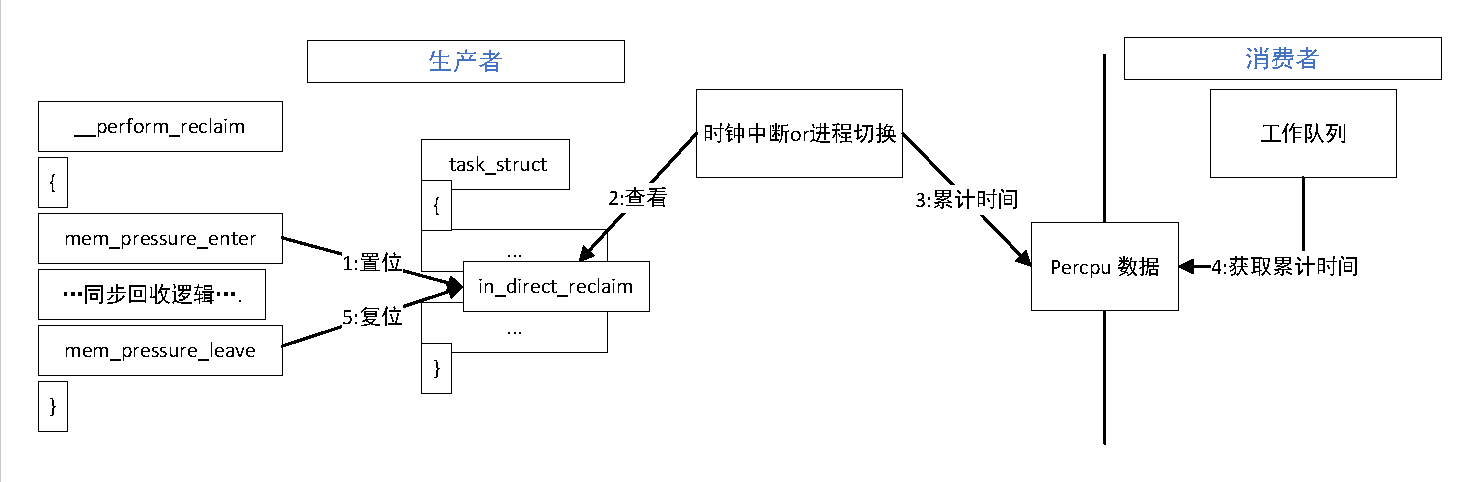
\includegraphics[width=\textwidth,keepaspectratio]{生产者和消费者.pdf}
    \caption{生产者消费者架构图}
    \label{fig:producer-consumer}
\end{figure}

系统实现如\ref{fig:producer-consumer}, 采用生产者消费者模式构建内存压力实时监控与评估框架。该模式通过解耦数据采集与数据处理两个核心功能模块。生产者模块负责采集内存回收过程中的时间片数据,而消费者模块则周期性地处理这些数据,计算内存压力指标。两者共享Per-CPU数据,它统计了每个CPU中发生内存同步回收的时间。具体的信息详见\ref{tab:sensor_data}。同时本文在 Linux 中 task\_struct 中 in\_mem\_mempressure 表示这个进程在处理同步内存回收了。

\begin{table}[htbp]
    \centering
    \caption{Per-CPU 变量}
    \label{tab:sensor_data}
    \begin{tabular}{ccc}
        \toprule
        成员名称& 数据类型     & 描述                                        \\ \midrule
        in\_direct\_reclaim & bool & 当前CPU是否处于同步内存回收状态\\
        \midrule
        time & u32 & 上一次累积时间的时间戳\\
        \midrule
        total\_time &u32&当前CPU处于同步内存回收状态的累积时间\\
        \midrule
        total\_time\_prev&u32&上一次统计时CPU处于同步内存回收状态的累积时间\\
        \midrule
        total\_work\_time&u32&当前CPU处于工作状态的累积时间\\
        \midrule
        total\_work\_time\_prev&u32&上一次统计时CPU处于工作状态的累积时间\\
        \bottomrule
    \end{tabular}
  \end{table}

生产者模块的核心功能是精确捕获内核中与内存回收相关的状态切换时间信息。为实现这一目标,生产者在同步内存回收的起始和结束时刻改变状态。具体而言,当系统发生直接内存回收时,即进程在分配内存时因内存不足而触发同步回收操作,生产者立即改变状态。当同步回收过程结束,进程恢复正常执行时,生产者再次改变状态,并计算累积时间。同时每次时钟中断的时候,它会进行累积时间。除此之外,生产者需要和调度系统交互,用来控制时钟中断收集间隔,因为当这个线程调度出去的时候,CPU就不会花费时间来处理同步内存回收,当调度进来的时候,生产者就需要重新计算,所以需要和调度系统交互并且在task\_struct中in\_mem\_mempressure标志来表示这个线程是否在处理同步内存回收。

消费者模块使用工作队列来实现,周期的从Per-CPU中读取读取,进行聚合,在\ref{sec:工作队列}介绍了选用工作队列的原因,在\ref{sec:内存压力计算算法}中介绍了详细的算法实现。


\subsection{生产者工作流程}

\begin{figure}[htbp]
    \centering
    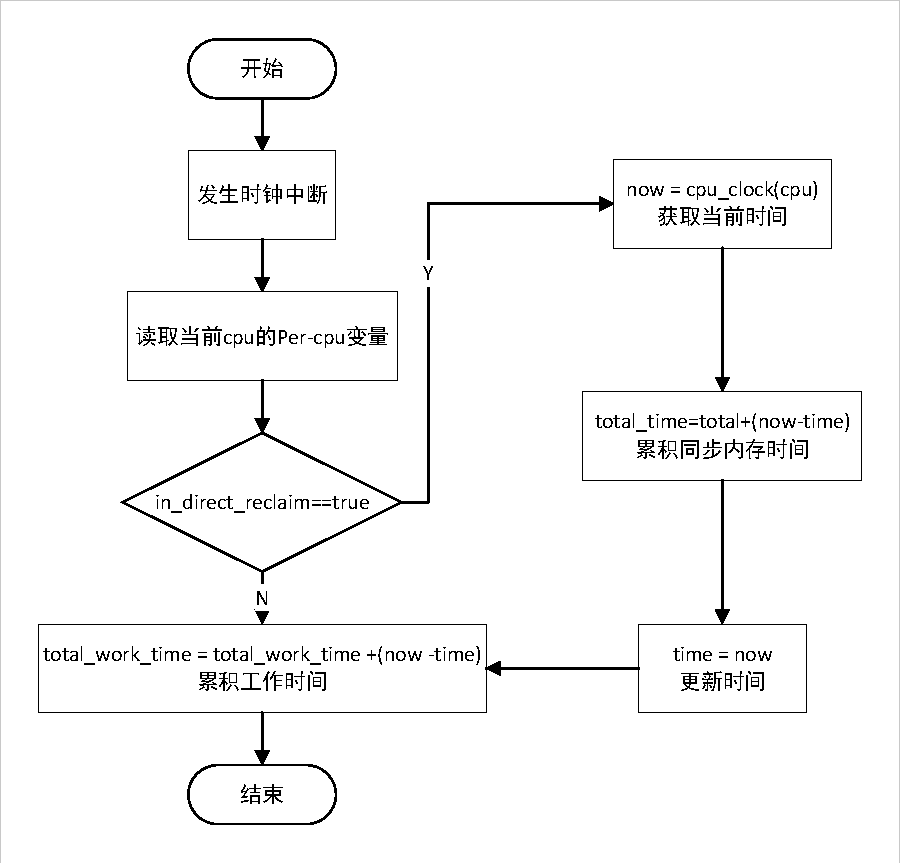
\includegraphics[width=0.8\textwidth,keepaspectratio]{时钟中断.pdf}
    \caption{时钟中断流程图}
    \label{fig:time-ticker}
\end{figure}
图\ref{fig:time-ticker} 所示为时钟中断处理流程。该流程始于时钟中断的触发,随后系统读取当前CPU的Per-CPU变量,并进入一个关键判定节点:判断in\_direct\_reclaim标志的状态。

若in\_direct\_reclaim为真,表明当前CPU正处于直接内存回收状态。此时,系统会执行以下操作:首先,通过cpu\_clock(cpu)函数获取当前时间戳,记为now;其次,计算时间差(now - time),并将其累加到total\_time变量中,用于统计同步内存回收所消耗的时间;最后,将now的值赋给time,以更新当前时间记录。这一过程确保了系统能够准确记录CPU在同步内存回收上花费的时间。

若in\_direct\_reclaim为假,则表明当前CPU未处于直接内存回收状态。此时,系统会计算时间差(now - time),并将其累加到total\_work\_time变量中,用于统计CPU在工作状态下的时间消耗。无论in\_direct\_reclaim的真假,流程最终都会汇聚至结束节点,完成一次时钟中断的处理。


此外,在进程切换时,系统会检查task\_struct中的in\_mem\_mempressure标志。如果当前进程的in\_mem\_mempressure为true,则表明该进程涉及内存压力,此时需要修改Per-CPU变量中的in\_direct\_reclaim标志,以表示当前CPU不再花费时间进行同步内存回收。反之,如果要切换进来的进程的in\_mem\_mempressure为true,则需要将Per-CPU变量中的in\_direct\_reclaim标志设置为true,表示当前CPU需要花费时间进行同步内存回收。

\subsection{消费者实现与并发安全保障}
\label{sec:consumer_implementation}

\subsubsection{基于工作队列的消费者实现}
\label{sec:工作队列}
在内存压力监控系统的消费者模块实现中,本文选择采用Linux内核工作队列机制,主要基于以下三方面考量:
\begin{enumerate}
    \item 内存压力计算过程涉及锁获取和较长时间的数据处理,必须在进程上下文中执行。工作队列提供的进程上下文执行环境,能够安全地处理可能引起睡眠的操作,这是中断上下文所不允许的。
    \item 压力监测需要周期性执行,工作队列的延迟执行机制(queue\_delayed\_work)不仅提供了高效的定时功能,还实现了完善的周期补偿。即使在系统负载较高导致某些执行周期被延迟时,工作队列能够通过公式(\ref{eq:missed_periods})计算错过的周期数并进行补偿,确保监测的连续性和数据的一致性。
    \item 工作队列的自适应特性使其能根据系统负载动态调整执行频率,在保证监测效果的同时最小化性能开销。相比于自行实现专用内核线程,工作队列机制显著降低了边界条件处理的复杂度,避免了诸如线程创建、销毁和唤醒等底层细节的处理。
\end{enumerate}

本文的实现使用以下工作队列API完成内存压力监测的周期性执行:

\begin{table}[htbp]
\centering
\caption{内存压力监测系统使用的工作队列API}
\label{tab:workqueue_api}
\begin{tabular}{cc}
\toprule
\textbf{API} & \textbf{在内存压力监测中的应用} \\
\midrule
alloc\_workqueue & 创建专用内存压力监测工作队列 \\
INIT\_DELAYED\_WORK & 初始化周期性监测任务 \\
queue\_delayed\_work & 按指定周期调度监测任务 \\
\bottomrule
\end{tabular}
\end{table}

具体而言,消费者模块通过工作队列周期性地调用算法\ref{alg:mem_pressure_optimized},依次执行多核加权聚合、时间戳更新和指数平滑计算,完成内存压力的实时评估。该实现不仅确保了监测过程的稳定性和可靠性,还使监测代码能够与工作负载高效共存,最小化了系统性能影响。

\subsubsection{临界区的保护}

在生产者消费者模型中,生产者负责采集内存回收过程中的累积时间,而消费者(工作队列)则负责处理这些数据,计算并输出内存压力指标。为了确保数据在并发环境下的完整性和一致性,同时兼顾性能,需要对临界区进行精细的保护。

在详细阐述临界区保护策略之前,简要介绍本研究所采用的核心同步机制:序列锁(Seqlock)。序列锁是 Linux 内核提供的一种轻量级同步原语,特别适用于读多写少且写操作简短的场景。其基本原理如图 \ref{fig:seqlock} 所示。序列锁维护一个序列计数器,写操作通过递增该计数器来标识数据更新的开始和结束(奇数表示写操作进行中,偶数表示无写操作)。读操作在开始时记录序列号 read\_seqbegin() ,并在读取完成后再次检查序列号 read\_seqretry() 。如果序列号发生变化,则表明在读取过程中发生了写操作,读操作需要重试,以确保读取到一致的数据。

\begin{figure}[H]
    \centering
    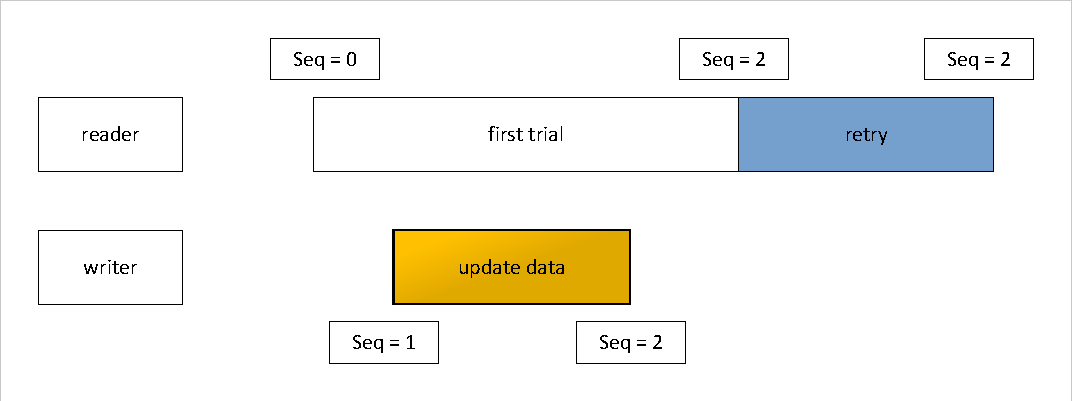
\includegraphics[width=\textwidth,keepaspectratio]{seqlock.pdf}
    \caption{序列锁(Seqlock)原理示意图}
    \label{fig:seqlock}
\end{figure}

该方案的选择主要基于以下多维约束分析:

\begin{enumerate}
    \item \textbf{Per-CPU 数据:} 每个 CPU 核心维护一份独立的数据结构,在表\ref{tab:sensor_data}中可以看到存储了CPU的统计信息。虽然 Per-CPU 变量在更新时本身具有原子性,无需额外加锁,但考虑到消费者需要读取所有 CPU 的 Per-CPU 数据进行聚合计算,因此仍需采取适当的同步措施。

    \item \textbf{全局统计信息:} 一个全局静态变量,用于存储所有 CPU 停顿时间的累加值,以及用于平滑计算的历史统计数据。该变量的访问涉及多个 CPU 的数据聚合,因此需要严格的保护。

    \item \textbf{ task\_struct->in\_mem\_mempressure  标志:} 进程描述符( task\_struct )中的一个标志位,用于标识当前进程是否涉及内存压力。用于指导每次进程切换的时候,是否需要更新Per-CPU中的in\_direct\_reclaim标志。
\end{enumerate}



基于对数据结构特点和访问模式的分析,本研究采用了三种针对性的临界区保护策略。

首先,对于Per-CPU数据中的累计时间,采用序列锁保护机制。选择序列锁的主要原因是时钟中断处理函数需要更新该数据,而中断处理程序不能被阻塞,序列锁正好提供了无阻塞写入能力。此外,Per-CPU数据结构相对简单,多为32位或64位无符号整型,写操作(累加时间)执行快速,读取时可整体复制,符合序列锁的适用条件。由于内存同步回收通常不是高频事件,对停顿时间的累加操作较少,构成典型的读多写少场景,与序列锁的设计理念高度契合。

其次,对于全局统计信息,本研究采用互斥锁(Mutex)保护。互斥锁提供了更强的互斥性,适合保护涉及较长计算时间或复杂数据结构的操作。全局统计信息的更新需要聚合多个CPU的数据并进行历史数据的平滑计算,这些操作相对耗时,因此互斥锁能有效确保数据的一致性和完整性。全局统计信息的访问频率相对较低,通常只在消费者周期性执行时进行,使用互斥锁的性能开销在可接受范围内。
\begin{algorithm}[htbp]
    \caption{Memory Pressure Calculation}
    \label{alg:mem_pressure_optimized}
    \SetAlgoLined
    \DontPrintSemicolon

    \Input{
            \(\text{total\_time}_i, \text{total\_time\_prev}_i, \text{total\_work\_time}_i, \text{total\_work\_time\_prev}_i\) (for each CPU \(i\));
            \(\text{mem\_pressure\_time}, \text{mem\_pressure\_time\_prev}\),
            \(\text{mem\_pressure\_prev}, \text{next\_update\_time}, \text{last\_update\_time}, T, \text{exp}\);
    }
    \Output{updated 
         \(\text{mem\_pressure\_prev}, \text{mem\_pressure\_time\_prev},\)
         \(\text{next\_update\_time}, \text{last\_update\_time}\)}

    \BlankLine

    \(\text{weight\_pressure\_time}, \text{work\_time} \gets \text{calculate\_weighted\_pressure\_time}(\text{cpu\_data})\)\;
    \(\text{mem\_pressure\_time} \gets \lfloor \text{weight\_pressure\_time}/\max(\text{work\_time},1)\rfloor\)\;

    \(\text{next\_update\_time}, \text{last\_update\_time}, \text{missed}, \text{period} \gets\) \(\text{update\_timestamps}(\text{sched\_clock}(), \text{next\_update\_time}, \text{last\_update\_time}, T)\)\;

    \(\text{mem\_pressure\_prev} \gets \text{exponential\_smoothing}(\)
    \qquad \(\text{mem\_pressure\_time}, \text{mem\_pressure\_time\_prev},\)
    \qquad \(\text{period}, \text{mem\_pressure\_prev}, \text{exp}, \text{missed})\)\;
\end{algorithm}
最后,对于 task\_struct 中的 in\_mem\_mempressure 标志,本研究利用运行队列锁进行隐式保护。该标志在同步内存回收开始时置位,结束时复位,这些操作通常发生在进程调度环境中。由于内核在操作过程中已持有相应CPU的运行队列锁并关闭本地中断,这自然形成了一道保护屏障,防止其它CPU或中断对当前进程的调度产生干扰。在时钟中断处理函数中检查该标志时,运行队列锁的存在保证了当前进程不会被调度到其它CPU,使得直接访问该标志是安全的,无需引入额外的锁机制。这种复用已有同步原语的策略,有效降低了系统的复杂度和同步开销。

通过上述针对性的临界区保护策略,本框架在确保数据一致性的前提下,最大限度地降低了同步开销,提升了系统的整体性能。

\subsection{内存压力计算工程实现}
\label{sec:内存压力计算算法}

本节聚焦于内存压力量化算法的工程实现。基于\ref{sec:基于同步内存回收延迟的内存压力量化算法}的理论模型,本文设计了一套高效的算法体系,实现了从原始数据采集到最终压力指标输出的完整计算流程。核心实现遵循先聚合、再校准、后平滑的处理逻辑,同时采用定点数运算优化性能。

算法\ref{alg:mem_pressure_optimized}展示了内存压力计算的主流程。第1行调用\\
 calculate\_weighted\_pressure\_time 函数实现\ref{sec:weighted_aggregation}节提出的多核加权聚合模型。第2行将加权后的内存压力时间转换为百分比表示,同时通过max函数处理工作时间为零的边缘情况。第3行调用 update\_timestamps 函数实现时间校准机制,处理采样周期偏移问题。第4行应用 exponential\_smoothing 函数实现指数平滑处理,输出最终压力值。

\begin{algorithm}[htbp]
\caption{calculate\_weighted\_pressure\_time}
\label{alg:calculate_weighted_pressure_time}
\SetAlgoLined
\DontPrintSemicolon
\Input{\(\text{total\_time}_i, \text{total\_time\_prev}_i, \text{total\_work\_time}_i, \text{total\_work\_time\_prev}_i\) (for each CPU \(i\))}
\Output{\(\text{weight\_pressure\_time}, \text{work\_time}\)}
\(\text{weight\_pressure\_time} \gets 0,\quad \text{work\_time} \gets 0\)\;
\For{each CPU \(i\)}{
    \(\text{weight\_pressure\_time} \gets \text{weight\_pressure\_time} + (\text{total\_time}_i - \text{total\_time\_prev}_i) \times (\text{total\_work\_time}_i - \text{total\_work\_time\_prev}_i)\)\;
    \(\text{work\_time} \gets \text{work\_time} + (\text{total\_work\_time}_i - \text{total\_work\_time\_prev}_i)\)\;
}
\Return{\(\text{weight\_pressure\_time}, \text{work\_time}\)}
\end{algorithm}

算法\ref{alg:calculate_weighted_pressure_time}实现了多核加权聚合。第3行是该算法的核心,它通过回收时间增量与工作时间增量的乘积累加,实现了公式\ref{eq:weighted_aggregation}中的权重聚合,避免了空闲核心的稀释效应。这种实现方式优于显式维护权重数组的方法,具有更高的计算效率。第4行累加工作时间增量,为后续计算压力百分比提供分母。


\begin{algorithm}[htbp]
\caption{update\_timestamps}
\label{alg:update_timestamps}
\SetAlgoLined
\DontPrintSemicolon
\Input{\(\text{now}, \text{next\_update\_time}, \text{last\_update\_time}, T\)}
\Output{ \(\text{next\_update\_time}, \text{last\_update\_time}, \text{missed}, \text{period}\)}
\If{\(\text{now} < \text{next\_update\_time}\)}{
\Return{\(\text{next\_update\_time}, \text{last\_update\_time}, 0, 0\)}
}
\(\text{missed} \gets \lfloor(\text{now}-\text{next\_update\_time})/T\rfloor\)\;
\(\text{next\_update\_time} \gets \text{next\_update\_time} + (\text{missed}+1) \times T\)\;
\(\text{period}\gets \text{now}-\text{last\_update\_time}\)\;
 \(\text{last\_update\_time}\gets \text{now}\)\;
\Return{\(\text{next\_update\_time}, \text{last\_update\_time}, \text{missed}, \text{period}\)}
\end{algorithm}

算法\ref{alg:update_timestamps}处理采样时间管理。第1-2行检查是否达到下次更新时间,避免过早执行。第3行根据公式\ref{eq:missed_periods}计算错过的周期数。第4行应用公式\ref{eq:next_execution}更新下次执行时刻,保持采样相位一致性,防止时间偏移累积。这种相位校准机制确保了即使在系统负载波动时,内存压力监测依然能保持连续稳定的采样节奏。
\begin{algorithm}[htbp]
\caption{exponential\_smoothing}
\label{alg:exponential_smoothing}
\SetAlgoLined
\DontPrintSemicolon
\Input{
    \begin{varwidth}{\linewidth}
      \(\text{mem\_pressure\_time}, \text{mem\_pressure\_time\_prev}, \text{period}\)\\
      \(\text{mem\_pressure\_prev}, \text{exp}, \text{missed}\)
    \end{varwidth}
}
\Output{\(\text{mem\_pressure\_prev}\)}

\(\text{sample\_time}\gets \text{mem\_pressure\_time}-\text{mem\_pressure\_time\_prev}\)\;
\If{\(\text{sample\_time}>\text{period}\)}{
    \(\text{sample\_time}\gets \text{period}\)
}
\(\text{mem\_pressure\_time\_prev} \gets \text{mem\_pressure\_time\_prev} + \text{sample\_time}\)\;
\(\text{tmp\_mem\_pressure}\gets \lfloor(\text{sample\_time}\times 100\times 2^{10})/\text{period}\rfloor\)\;
\If{\(\text{missed}>0\)}{
  \(\text{exp} \gets \text{fixed\_power\_int}(\text{exp}, \text{missed})\)
}
\(\text{new\_mem\_pressure}\gets \text{mem\_pressure\_prev}\times \text{exp} + \text{tmp\_mem\_pressure}\times(2^{10}-\text{exp})\)\;
\If{\(\text{mem\_pressure\_prev}>\text{tmp\_mem\_pressure}\)}{
  \(\text{new\_mem\_pressure} \gets \text{new\_mem\_pressure} + (2^{10}-1)\)
}
\(\text{mem\_pressure\_prev}\gets \lfloor \text{new\_mem\_pressure}/2^{10}\rfloor\)\;
\Return{\(\text{mem\_pressure\_prev}\)}
\end{algorithm}

算法\ref{alg:exponential_smoothing}实现了指数平滑处理。第1-2行计算并限制样本时间,应用\ref{sec:time_calibration_and_data_processing}节提出的截断补偿机制。第4行将样本时间转换为百分比并用定点数表示,实现\ref{sec:fixed_point_optimization}节的定点数优化。第5-6行处理连续多个周期未更新的情况,使用fixed\_power\_int函数实现指数加速收敛。第7行使用指数加权公式计算新的内存压力值,定点数表示的exp和$(2^{10}-\text{exp})$分别对应公式\ref{eq:EMA}中的\(\alpha\)和\((1-\alpha)\)。第8-9行是工程优化,在压力下降时进行微调,提高系统对压力缓解的响应性。
\SetKwFunction{FixedPowerInt}{fixed\_power\_int}
\SetKwProg{Fn}{Function}{:}{}
\begin{algorithm}[htbp]
    \caption{fixed\_power\_int}
    \label{alg:helper_functions}
    \SetKwFunction{FixedPowerInt}{fixed\_power\_int}
    \SetKwProg{Fn}{Function}{:}{}

    \Fn{\FixedPowerInt(\(x\), \(n\))}{
        \(result \gets 2^{10}\) \;
        \If{\(n > 0\)}{
            \While{true}{
                \If{\((n \land 1) \neq 0\)}{
                    \(result \gets (result \times x + 2^9) \gg 10\)\;
                }
                \(n \gets n \gg 1\)\;
                \If{\(n = 0\)}{\textbf{break}}
                \(x \gets (x \times x + 2^9) \gg 10\)\;
            }
        }
        \Return \(result\)\;
    }
\end{algorithm}
算法\ref{alg:helper_functions}实现了定点数快速幂计算。第2行初始化结果为定点数的1.0。第3-11行实现二进制快速幂算法,时间复杂度为$O(\log n)$。第6行和第9行中的$(expr + 2^9) \gg 10$操作实现了定点数乘法中的四舍五入,确保计算精度。




\section{本章小结}
本章详细阐述了基于同步内存回收延迟的内存压力量化算法的设计与实现。首先,通过分析同步回收延迟与内存压力的关联性,提出了基于同步回收延迟的内存压力量化模型,并建立了相应的数学表征。其次,针对多核系统中的负载不均衡问题,设计了多核加权聚合算法,有效降低了空闲核心对压力评估的干扰。此外,引入指数移动平均算法对压力数据进行平滑处理,减少了短期波动的影响,同时采用定点数优化技术显著提升了计算效率。在实现层面,基于生产者消费者模式构建了内存压力实时监控框架,通过序列锁和互斥锁等同步机制确保了数据的一致性和完整性。最后,详细介绍了内存压力计算算法的具体实现,包括加权压力时间计算、时间戳更新以及指数平滑更新等核心模块。
\chapter{基于内存压力的自动卸载框架}
\label{chap:基于内存压力的自动卸载框架}
在\ref{chap:基于同步内存回收的内存压力量化算法的设计与实现}中,已将同步内存回收量化为内存压力。基于量化的压力值,用户态的内存压力感知卸载框架可以主动将冷页面卸载到异构后端。本章将介绍基于proc文件系统的mpfs实现、基于内存压力的工作集估计算法以及基于访问距离的匿名页和文件页的平衡算法。


\section{内存压力文件系统的实现}
\label{sec:mpfs_implementation}

基于\ref{sec:基于同步回收延迟的内存压力量化实现}章节实现的内存压力量化模型,本节构建用户态调控接口以实现冷页面的动态卸载机制。选择用户态实现方案可有效提升策略迭代效率,同时支持基于 QoS 需求的差异化策略配置。

\subsection{proc 文件系统架构分析}

proc 文件系统作为内核与用户态间的标准交互接口,其设计具有以下核心特征:

\begin{itemize}
    \item \textbf{动态生成机制:} 文件节点根据内核运行时状态实时构建
    \item \textbf{虚拟存储特性:} 不占用物理存储空间,通过内存映射实现数据存取
    \item \textbf{双向交互能力:} 支持通过标准I/O系统调用进行内核参数查询与配置
    \item \textbf{抽象访问层:} 对用户态程序隐藏内核数据结构复杂性,提供统一访问范式
\end{itemize}

上述特性使其成为实现跨态内存压力交互的理想媒介。

\subsection{mpfs 系统架构设计}

本系统通过设计内存压力文件系统(Memory Pressure File System, mpfs)实现以下核心功能:

\begin{itemize}
    \item \texttt{/proc/mpfs/mem\_pressure}:提供实时内存压力值轮询接口,支持事件驱动通知机制
    \item \texttt{/proc/mpfs/period}:实现采样周期动态可配置接口(时间单位:秒)
    \item \texttt{/proc/mpfs/mthreshold}:设置压力阈值触发条件(百分比形式)
\end{itemize}

表 \ref{tab:mpfs_files} 详细描述了各文件接口的操作语义及功能映射关系。

\begin{table}[H]
    \centering
    \caption{mpfs 文件系统接口规范}
    \label{tab:mpfs_files}
    \begin{tabular}{lccc}
        \toprule
        \textbf{操作类型} & \texttt{mem\_pressure} & \texttt{period} & \texttt{mthreshold} \\
        \midrule
        \texttt{read} & 读取当前压力值 & 获取采样周期 & 查询当前阈值 \\
        \texttt{write} & - & 更新采样周期 & 修改触发阈值 \\
        \texttt{poll} & 事件通知机制 & - & - \\
        \bottomrule
    \end{tabular}
\end{table}

\subsection{内核模块实现细节}

系统通过注册内核模块实现功能组件,核心流程如下:

\begin{itemize}
    \item \textbf{模块初始化:} 通过 \texttt{proc\_create} 在 \texttt{/proc/mpfs} 目录下创建三个虚拟文件节点,分别绑定对应的文件操作函数集(\texttt{file\_operations})
  
    \item \textbf{压力值读取:}
    \begin{itemize}
        \item \texttt{mempressure\_read} 函数从原子变量 \texttt{current\_usage\_percent} 获取压力值
        \item 采用 \texttt{sprintf} 格式化输出保证数据可读性
    \end{itemize}

    \item \textbf{事件通知机制:}
    \begin{itemize}
        \item \texttt{mempressure\_poll} 将进程加入等待队列 \texttt{mem\_waitq}
        \item 当工作队列计算出压力值后,如果超出了阈值,将唤醒等待队列 \texttt{mem\_waitq} 上的所有进程
        \item 当 \texttt{pressure\_flag} 置位时返回 \texttt{POLLIN | POLLRDNORM} 状态码
    \end{itemize}

    \item \textbf{参数动态配置:}
    \begin{itemize}
        \item 采样周期更新函数 \texttt{mempressure\_period\_write} 包含整型参数校验逻辑
        \item 阈值修改函数 \texttt{mempressure\_threshold\_write} 实施百分比有效性验证
    \end{itemize}
\end{itemize}

该架构通过标准文件接口实现用户态策略与控制参数的动态注入,同时保证内核态监测机制的实时响应能力。



\section{基于内存压力的动态调控模型}
\label{sec:pressure_based_model}

传统工作集估计方法依赖内核态时间、应用吞吐量变化率、回收事件计数器等间接指标,其有效性受限于运维人员对存储硬件特性与内核行为的专业认知。在\ref{chap:基于同步内存回收的内存压力量化算法的设计与实现}中,本研究提出基于同步内存回收的压力指标,可以自适应不同的负载和异构卸载后端。本节我们就基于定义的内存压力,来实现基于内存压力的动态调控。此模型采用主动回收策略,通过监控系统内存压力来维持目标压力区间,并将低访问频率数据页迁移至基于`frontswap`的异构存储后端,从而实现内存利用率的优化。

\begin{figure}[h]
\centering
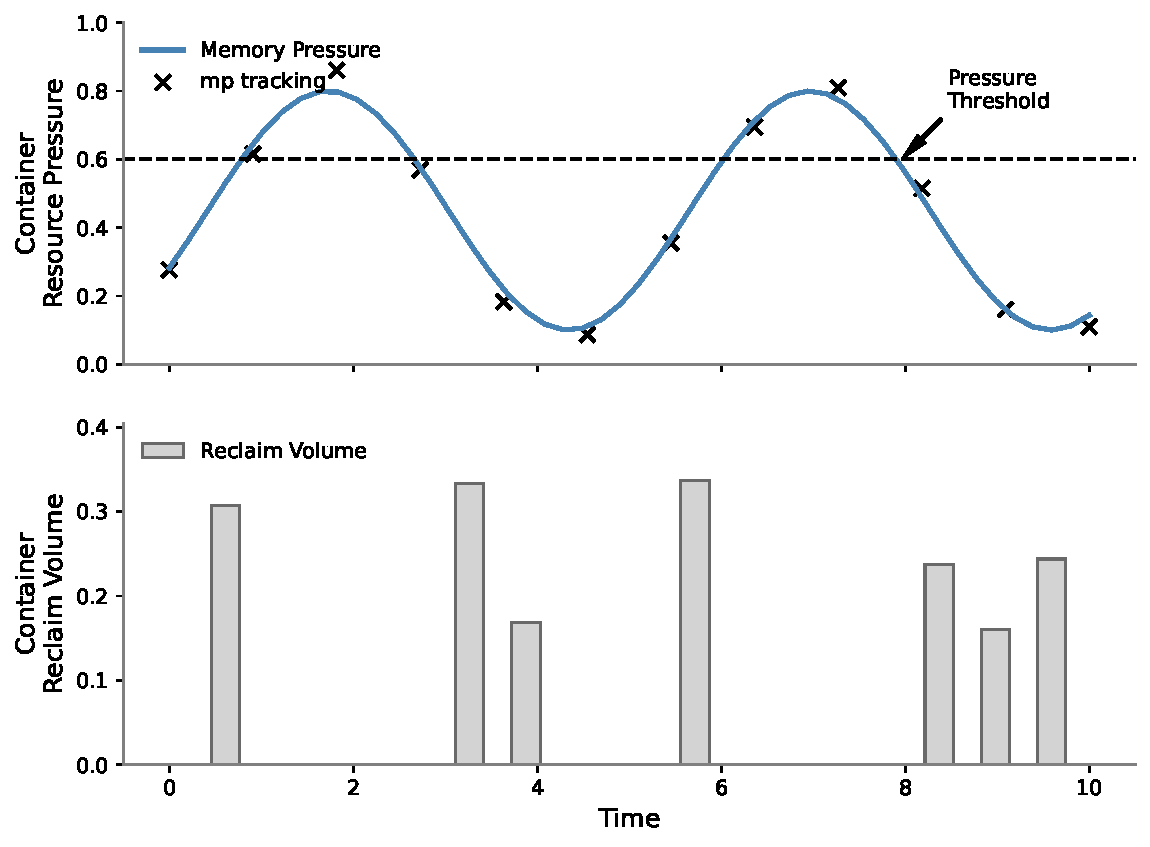
\includegraphics[width=0.95\textwidth]{压力与回收.pdf}
\caption{内存压力与页面回收调控机制}
\label{fig:pressure_work_set}
\end{figure}

本算法通过压力量化与反馈机制来实现内存的动态调控。不同于传统的静态内存管理策略,本算法根据系统的实时内存压力调整内存的使用范围,确保系统在高负载时能够扩展内存资源,在低负载时又能将冷页面主动卸载。这种基于内存压力的调控方法能够有效应对突发负载变化,并在保证系统稳定性的同时,提高内存资源的利用率。

图\ref{fig:pressure_work_set}展示了本模型的设计目标,即通过监控系统的内存压力,采用动态调整策略,确保系统内存处于合理的使用范围内。具体而言,当系统内存压力超过设定目标时,系统会逐步放宽内存限制;反之,内存压力较低时,系统会收紧内存限制。这样,不仅能在高负载时避免内存不足的问题,还能在低负载时将冷页面主动卸载。

本算法采用压力积分反馈机制,其中的关键参数体系如表\ref{tab:params}所示。算法每6秒钟执行一次,设定一个目标内存压力阈值,实现系统的平滑调节。累积的压力误差是通过比较实际内存压力与目标内存压力阈值的差异来计算的,从而形成一个时间窗口内的压力累积效应。



\begin{table}[H]
\centering
\caption{调控参数体系}
\label{tab:params}
\begin{tabular}{cccc}
\toprule
参数 & 符号 & 默认值 & 作用域 \\
\midrule
目标压力 & \(mem\_pressure\_target\) & 0.1\% & 全局 \\
最大收缩率 & \(M_p\) & 0.01 & 缩容阶段 \\
最大扩张率 & \(M_b\) & 1.0 & 扩容阶段 \\
收缩灵敏度 & \(C_p\) & 10 & 缩容触发 \\
扩张灵敏度 & \(C_b\) & 20 & 扩容触发 \\
\bottomrule
\end{tabular}
\end{table}

\begin{algorithm}[H]
    \caption{基于压力的内存调控算法}
    \label{alg:control}
    \Input{\(mem\_pressure\), \(mem\_pressure\_target\), \(C_b\), \(C_p\), \(M_b\), \(M_p\), \(min\_size\), \(max\_size\)}
    \Output{Memory Limit \(Limit\)}
    \While{\textrm{true}}{  
        \(mem\_pressure\) get from proc file system;\\
        \If{\(mem\_pressure > mem\_pressure\_target\)}{
            % Calculate expansion coefficient eta
            \(\eta \leftarrow \min\left(\left(\frac{mem\_pressure/mem\_pressure\_target}{C_b}\right)^2, 1\right)\)*\(M_b\)\;
            % Perform expansion
            \(Limit \leftarrow \min(max\_size, Limit \times (1 + \eta))\)\;
            }
        \Else{
            % Calculate contraction coefficient eta
            \(\eta \leftarrow \min\left(\left(\frac{mem\_pressure\_target/mem\_pressure}{C_p}\right)^2, 1\right)\)*\(M_p\)\;
            % Perform contraction
            \(Limit \leftarrow \max(min\_size, Limit \times (1 - \eta))\)\;
            }
        % Apply the new memory limit
        Apply new memory limit \(Limit\)\;
    }
\end{algorithm}

\begin{itemize}
\item \textbf{灵敏度系数(\(C_p, C_b\))}: 
  \begin{itemize}
  \item 扩张灵敏度\(C_b=20\): 当累积压力超过目标值20倍时达到最大扩容比例
  \item 收缩灵敏度\(C_p=10\): 当压力低于目标值1/10时触发最大缩容
  \end{itemize}

\item \textbf{最大比例(\(M_p, M_b\))}: 
  \begin{itemize}
  \item \(M_b=1.0\)允许单次扩容100\%,应对突发压力
  \item \(M_p=0.01\)限制单次缩容1\%,确保服务稳定性
  \end{itemize}

\item \textbf{积分机制}: 
  \begin{itemize}
  \item 累积窗口\(T_{interval}=6s\)平滑瞬时波动
  \item 压力增量\(\Delta P\)累计检测持续负载
  \end{itemize}
\end{itemize}

本算法的设计考虑了内存压力的动态变化与不同负载场景下的需求,因此参数体系中包含了多种灵敏度、最大收缩比例、扩张比例等调控因子,用于灵活应对系统的负载变化。例如,扩张灵敏度\(C_b = 20\)表示当实际内存压力超过目标压力的20倍时,系统会达到最大扩容比例;收缩灵敏度\(C_p = 10\)则表示当实际内存压力低于目标压力的1/10时,系统会触发最大缩容。

最大扩张比例\(M_b = 1.0\)允许单次扩容至最大限制的100\%,应对突发的内存压力;而最大收缩比例\(M_p = 0.01\)限制单次缩容不超过1\%,确保系统的稳定性,避免因过快的收缩而导致服务质量下降。通过这些参数的调整,系统能够灵活应对不同的负载条件,避免内存资源的过度浪费,并确保在需要时能够快速扩展内存。


需要特别强调的是,上述算法只是一个示例,目的是展示如何基于内存压力进行动态调控。在实际应用中,用户可以根据不同的服务质量(QoS)要求、系统负载特性或硬件架构,单独配置这些参数,甚至根据负载类型重新定义内存调控策略。例如,在某些高实时性应用中,可能会选择较高的扩张灵敏度 \(C_b\) 和较低的收缩灵敏度 \(C_p\),以确保快速响应压力变化。而在对于一般后台任务的处理上,则可能会选用较为保守的策略,以确保稳定性和节省资源。

通过采用灵活配置的方式,本算法能够根据不同的需求调整内存压力阈值、调节因子和策略参数,从而提供更具针对性和适应性的内存管理策略。算法的灵活性使得它能够适用于不同的负载场景和硬件环境,满足各种不同应用的内存管理需求。

此外,该算法可以结合不同的内存管理机制,如基于事件驱动的非阻塞方法,避免轮询带来的性能损失。未来也可以通过引入机器学习或预测算法,自动调整调控策略和参数,以实现更加智能和自适应的内存管理。算法本身也可以与其他资源管理策略结合,共同优化系统的整体性能和资源分配。
、
% \section{内存压力文件系统的实现}
% \label{sec:mpfs_implementation}

% 在\ref{sec:基于同步回收延迟的内存压力量化实现}中,本研究已经实现了基于同步回收延迟的内存压力量化实现,我们需要根据压力来进行调控,实现冷页面的自动卸载。在用户态实现可以更快进行迭代,也可以根据负载的实际的QOS来设置不同的策略。

% 所以本研究需要将压力的值暴露给用户态,通过proc文件系统来实现是一个很好的方法。

% \subsubsection{proc 文件系统概述}

% proc 文件系统是一种特殊的、由内核动态生成的伪文件系统,通常挂载于 /proc 目录。它并不存储在物理磁盘上,而是存在于内存中,为用户空间提供了一种访问和修改内核信息的标准接口。proc 文件系统具有以下几个关键特性:

% \begin{itemize}
%     \item \textbf{动态性:} proc 文件系统中的文件和目录并非静态存在,而是由内核根据当前系统状态动态生成。
%     \item \textbf{虚拟性:} proc 文件系统中的文件不占用实际的磁盘空间,它们只是内核数据的虚拟表示。
%     \item \textbf{交互性:} 用户可以通过标准的文件 I/O 操作(如 \texttt{read}、\texttt{write}、\texttt{poll} 等)与 proc 文件系统中的文件进行交互,从而读取内核信息或修改内核参数。
%     \item \textbf{通用性:} proc 文件系统提供了一套统一的接口,使得用户空间的应用程序无需了解内核内部的复杂数据结构,即可方便地访问内核信息。
% \end{itemize}

% 基于 proc 文件系统的这些特性,它非常适合作为用户态与内核态之间进行信息交换的桥梁。

% \subsubsection{mpfs 的设计与实现}

% \texttt{mpfs} 的设计目标是提供一个轻量级、响应及时的接口,供用户态程序获取和监控系统的内存压力信息,并支持基于内存压力的事件通知机制。为了实现这一目标,\texttt{mpfs} 提供了以下三个文件接口:

% \begin{itemize}
%     \item \texttt{/proc/mpfs/mem\_pressure}:用于读取当前系统的内存压力值(百分比)。该文件支持 poll 系统调用,当内存压力超过预设阈值时,会触发可读事件,从而通知等待中的用户态程序。
%     \item \texttt{/proc/mpfs/period}:用于读取和设置内存压力采样周期(单位:秒)。用户态程序可以通过写入该文件来动态调整采样频率。
%     \item \texttt{/proc/mpfs/mthreshold}:用于读取和设置内存压力阈值(百分比)。当内存压力超过该阈值时,\texttt{/proc/mpfs/mem\_pressure} 文件的 poll 调用会返回可读事件。
% \end{itemize}

% 表 \ref{tab:mpfs_files} 总结了 mpfs 中各个文件接口及其对应的文件操作函数。

% \begin{table}[H]
%     \centering
%     \caption{mpfs 文件接口及操作}
%     \label{tab:mpfs_files}
%     \begin{tabular}{cccc} % 四列,都居中对齐
%         \toprule
%         \textbf{操作} & \textbf{\texttt{/proc/mpfs/mem\_pressure}} & \textbf{\texttt{/proc/mpfs/period}} & \textbf{\texttt{/proc/mpfs/mthreshold}} \\
%         \midrule
%         \texttt{read} & 获取内存压力 & 获取采样周期 & 获取压力阈值 \\
%         \texttt{write} &  & 设置采样周期 & 设置压力阈值 \\
%         \texttt{poll} & 内存压力事件通知 &  &  \\
%         \bottomrule
%     \end{tabular}
% \end{table}


% mpfs 的核心实现基于内核模块机制。在模块初始化函数 (mempressure\_init) 中,通过 proc\_create 函数创建了上述三个文件节点,并分别指定了它们的文件操作函数集(file\_operations 结构)。

% \begin{itemize}
%     \item \textbf{\texttt{mem\_pressure}} 文件:
%     \begin{itemize}
%         \item \texttt{read} 操作:调用 \texttt{mempressure\_read} 函数,从全局静态变量处获取当前内存压力值,并将其格式化为字符串后复制到用户空间缓冲区。
%         \item \texttt{poll} 操作:调用 \texttt{mempressure\_poll} 函数,该函数首先将当前进程添加到等待队列 \texttt{mem\_waitq} 中,然后调用\texttt{mempressure\_read}查看内存压力,。如果内存压力超过阈值,则返回 \texttt{POLLIN | POLLRDNORM},表示文件可读;否则,进程将进入睡眠状态,等待被唤醒。
%     \end{itemize}

% \item \textbf{\texttt{period}} 文件:
%     \begin{itemize}
%         \item \texttt{read} 操作:调用 \texttt{mempressure\_period\_read} 函数,该函数读取全局变量 \texttt{sample\_period}(采样周期,单位:秒),并将其格式化为字符串后复制到用户空间缓冲区。
%         \item \texttt{write} 操作:调用 \texttt{mempressure\_period\_write} 函数,该函数从用户空间缓冲区读取新的采样周期值,并进行合法性检查(必须为正整数)。然后更新采样周期,等到之后工作队列就可以采用新的采样周期。
%     \end{itemize}

%     \item \textbf{\texttt{mthreshold}} 文件:
%     \begin{itemize}
%     \item \texttt{read} 操作:调用 \texttt{mempressure\_threshold\_read} 函数,该函数读取全局变量 \texttt{mem\_pressure\_threshold}(内存压力阈值,百分比),并将其格式化为字符串后复制到用户空间缓冲区。
%     \item \texttt{write} 操作:调用 \texttt{mempressure\_threshold\_write} 函数,该函数从用户空间缓冲区读取新的阈值,并进行合法性检查)。然后更新阈值就可以返回。
%     \end{itemize}
% \end{itemize}

% 内存压力的周期性监测和事件通知由工作队列 \texttt{pressure\_work} 实现。工作队列的处理函数 \texttt{mempressure\_workfunc} 执行以下操作:

% \begin{enumerate}
%     \item 获取系统内存信息(总内存、可用内存),计算内存使用率(百分比)。
%     \item 将计算得到的内存使用率更新到原子变量 current\_usage\_percent。
%     \item 检查内存使用率是否超过阈值 mem\_pressure\_threshold。如果超过,则设置内存压力标志 pressure\_flag,并通过 wake\_up\_interruptible 函数唤醒等待队列 mem\_waitq 上的所有进程。
%     \item 根据当前采样周期 sample\_period 重新调度工作队列 pressure\_work。
% \end{enumerate}

% 通过上述设计和实现,mpfs 为用户态程序提供了一个简洁、高效的接口,用于实时监控系统内存压力,并根据需要调整采样周期和阈值。



\section{基于重用距离的冷热页面优化}
\label{sec:基于重用距离的冷热页面优化}


% \subsection{重用距离}

% 受到文献\cite{jiang2002lirs,jiang2005clockpro}关于重用距离(Reuse Distance)研究的启发,我们尝试引入重用距离这一概念来平衡文件页面与匿名页面的回收策略。重用距离刻画了某个页面两次访问之间,被访问过的不同页面的数量,能从更广阔的角度度量页面的使用频率及其在内存替换时的优先级。

% 对一段内存访问序列
% \[
%     A = \{a_1,\, a_2,\, a_3,\dots,a_n\},
% \]
% 令 \(a_i\) 表示第 \(i\) 次访问的页面编号。页面 \(P\) 的重用距离可定义为
% \begin{equation}
%   \label{eq:rd_def}
%   RD(P) \;=\; \min \bigl\{\, j - i \,\bigm|\,
%   a_i = P,\; a_j = P,\; i < j \bigr\},
% \end{equation}
% 即在页面 \(P\) 第一次被访问(索引 \(i\))到第二次被访问(索引 \(j\))之间,出现的不同页面数的最小可能值。若某页面的重用距离很短,则意味着其访问非常频繁;若重用距离较长,则该页面在替换算法中往往是更好的回收对象。

% \begin{figure}[htbp]
%   \centering
%   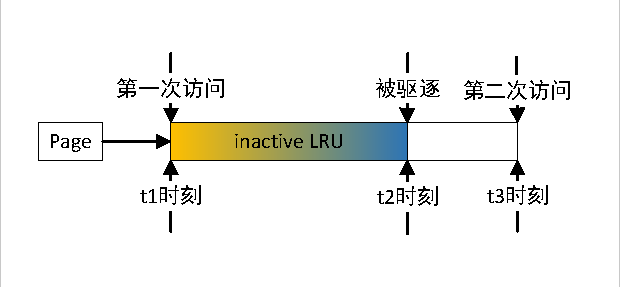
\includegraphics[width=0.5\textwidth]{重用距离.pdf}
%   \caption{重用距离示意图}
%   \label{fig:refault_distance}
% \end{figure}

% 然而,在实践中逐页追踪重用距离往往需要为每一页维护完整的历史访问信息,这在大型系统中会带来可观的存储和维护成本。为了降低开销,我们采用近似方法:观察页面在活动链表(Active List)和非活动链表(Inactive List)之间的迁移,以推断其访问频度;当页面重新被访问时,若该页面曾被替换出去(即从非活动链表被驱逐),则说明在它被驱逐至再次访问的这段时间里,系统至少经历了一定数量的页面访问。

% \subsection{重用距离的近似推导}

% 为了直观地分析非活动链表上的页面行为,我们做如下简化假设:非活动链表长度固定,且暂不考虑活动链表中的页面降级至非活动链表的情形。这样可更专注于分析非活动链表本身的访问与替换规律。在此前提下,图 \ref{fig:现象1} 与图 \ref{fig:现象2} 展示了两种典型场景:

% \begin{figure}[htbp]
%   \centering
%   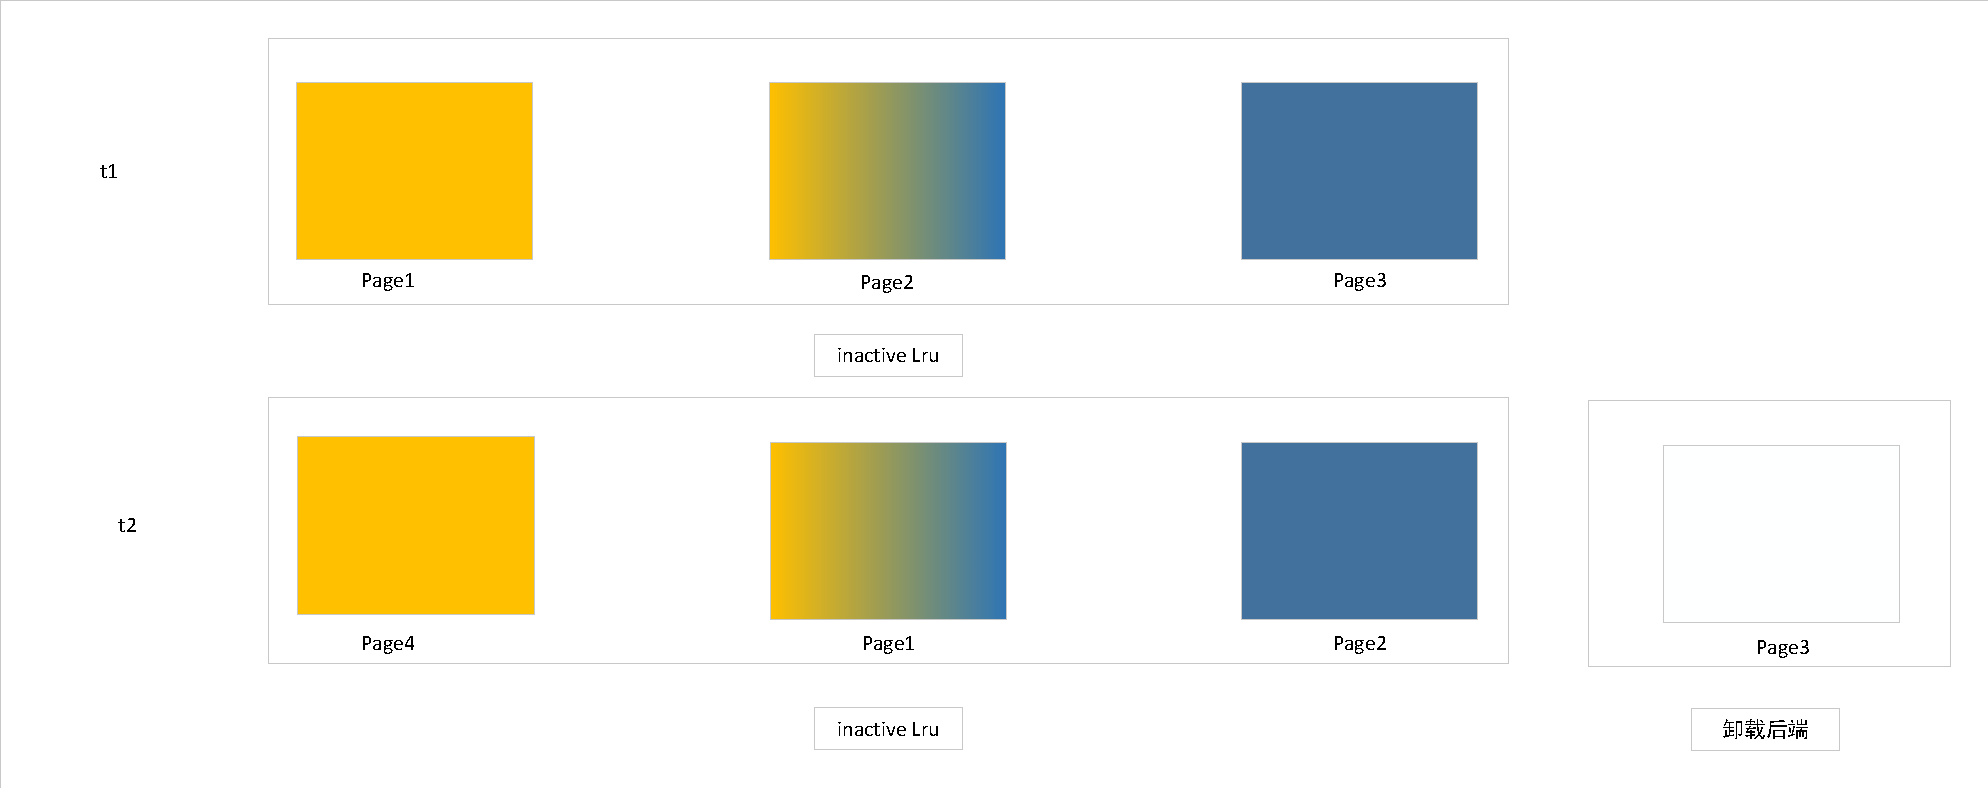
\includegraphics[width=0.5\textwidth]{现象1.pdf}
%   \caption{情形一:页面首次插入非活动链表}
%   \label{fig:现象1}
% \end{figure}

% \begin{figure}[htbp]
%   \centering
%   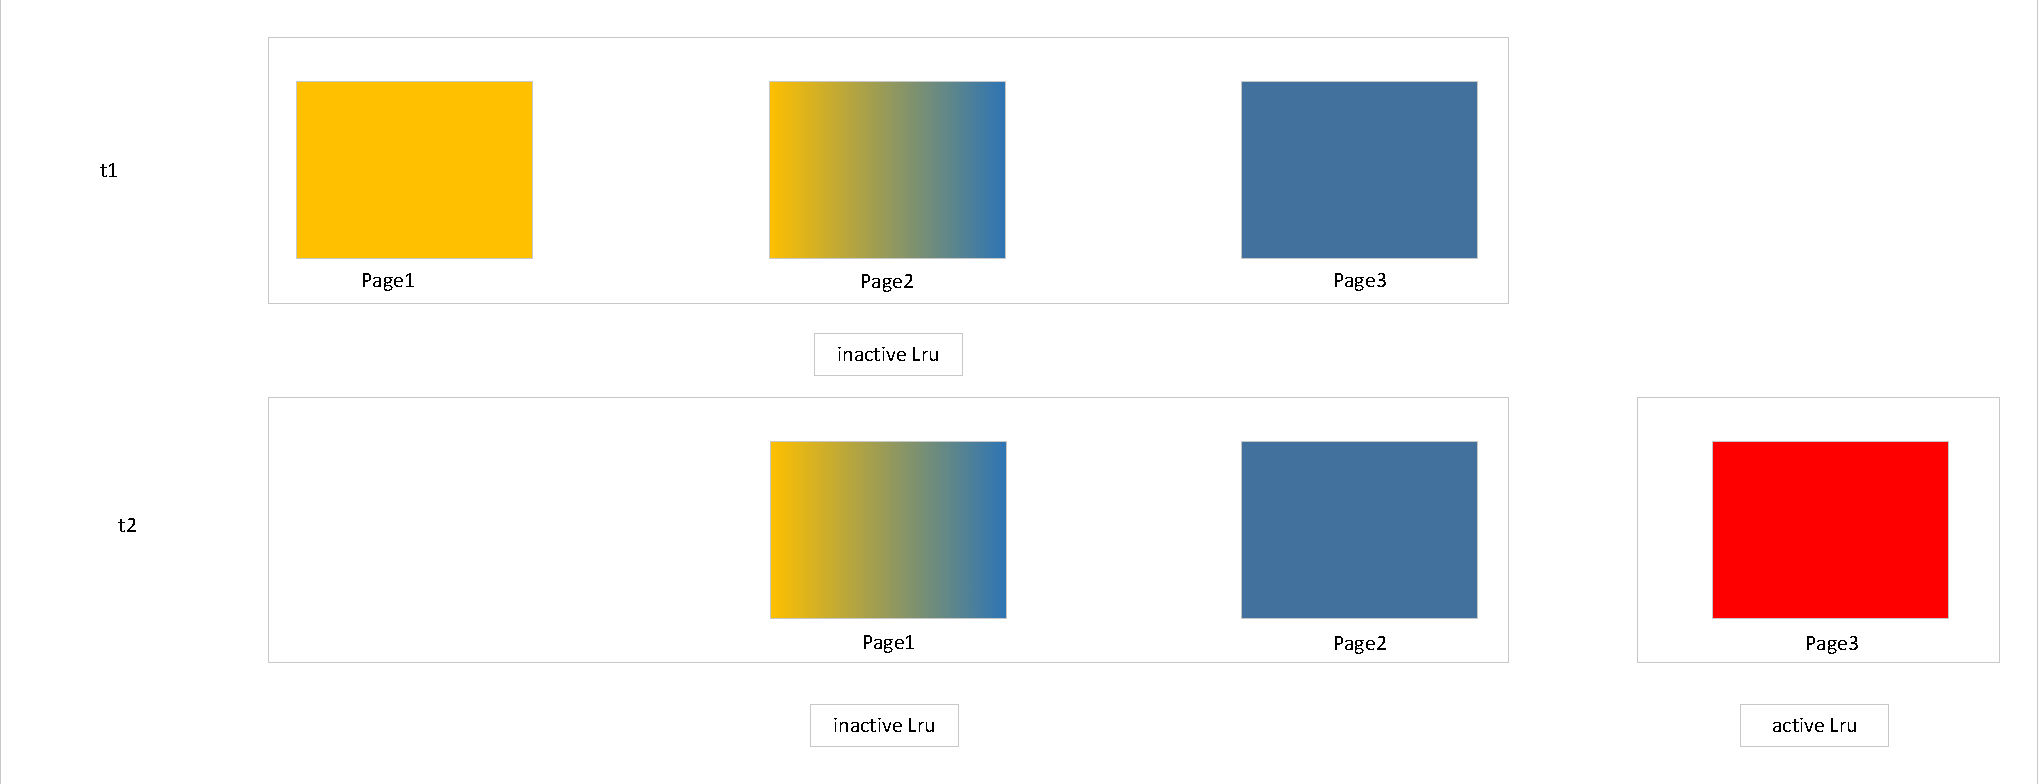
\includegraphics[width=0.5\textwidth]{现象2.pdf}
%   \caption{情形二:页面在非活动链表上再次被访问并提升到活动链表}
%   \label{fig:现象2}
% \end{figure}
% \begin{itemize}
%   \item 情形一(图 \ref{fig:现象1})对应页面第一次访问并被插入到非活动链表头部。由于非活动链表长度固定,原先在链表中的页面会整体向尾部滑动,最终导致最末尾的页面被挤出内存(即被驱逐)。  
%   \item 情形二(图 \ref{fig:现象2})对应页面在非活动链表上再次被访问并提升到活动链表,这同样会使非活动链表缩短一个位置,同时,所有比被提升页面更晚载入非活动链表的页面都会被推向尾部,从而离被驱逐更近。
% \end{itemize}

% 基于这两种主要行为,可以观察到:在时间区间 \([t_1, t_2]\) 内,非活动链表的页面要么被驱逐(表明一定有新页面加载)、要么被提升至活动链表(表明其被再次访问)。令
% \(
%   E(t_1,t_2)
% \)
% 表示在 \([t_1,t_2]\) 区间内的驱逐次数(evictions),令
% \(
%   A(t_1,t_2)
% \)
% 表示在该区间的页面提升次数(activations)。由于每次驱逐意味着至少加载了一个新的页面,每次提升代表至少发生了一次对非活动链表中页面的访问,故可以近似认为,在 \([t_1,t_2]\) 时间段里,系统产生的最少页面访问数不低于
% \begin{equation}
%   E(t_1,t_2) \;+\; A(t_1,t_2).
% \end{equation}
% 在实际系统中,尚需考虑其他潜在行为,例如“始终位于活动链表且未被降级的页面访问数”。不过,对于那些访问特别频繁的页面,因其始终活跃,我们往往无需担心它们被回收或缺少统计;换言之,这部分页面对近似分析的影响有限,而我们更需要关注的是可能进入或留在非活动链表的页面。



% % \paragraph{重新故障距离 的定义与计算}

% 当一个页面 \(p\) 被驱逐时,我们在驱逐时刻 \(t_1\) 记录一个计数器值 \({count}(t_1)\),它反映的是系统自启动至 \(t_1\) 时刻所累计的“驱逐次数 + 提升次数”(即 \(E + A\))。一旦该页面在时刻 \(t_2\) 再次被访问,我们同样记录 \({count}(t_2)\)。基于前述分析,可定义页面 \(p\) 的重新故障距离(Refault Distance)为
% \begin{equation}
%   \label{eq:refault_distance}
%   D_{\mathrm{refault}}(p)
%   \;=\;
%   \mathrm{count}(t_2)
%   \;-\;
%   \mathrm{count}(t_1),
% \end{equation}
% 它衡量了页面在被驱逐后到再次访问期间,系统所经历的最少页面访问数量。

% 若我们进一步近似页面在内存中的时候访问的页面数量使用非活动链表中的位置数 \(\displaystyle L_{\mathrm{inactive}}\),则可近似推断页面 \(p\) 的总“访问距离”为
% \begin{equation}
%   \label{eq:dtotal}
%   D_{\mathrm{total}}(p)
%   \;=\;
%   L_{\mathrm{inactive}}
%   \;+\;
%   \bigl(\mathrm{count}(t_2) - \mathrm{count}(t_1)\bigr).
% \end{equation}
% 其中,\(\displaystyle L_{\mathrm{inactive}}\) 是用来衡量“页面在非活动链表中一旦越往后排,就越接近被驱逐”的事实。直观来看,若非活动链表本身长度较小且页面常被迅速驱逐,那么一段时间内的 \(\mathrm{count}(\cdot)\) 增量就会变大,说明系统在该时段里确实经历了大量访问,也意味着较长的重用距离或低访问频度。

% \subsection{替换决策与回收策略}

% 结合活动链表的大小 \(\displaystyle L_{\mathrm{active}}\) 进行分析,若我们希望某页面在内存中继续保留,则需要满足
% \begin{equation}
%   \label{eq:active_condition}
%   L_{\mathrm{inactive}}
%   \;+\;
%   \bigl(\mathrm{count}(t_2) - \mathrm{count}(t_1)\bigr)
%   \;\;\le\;\;
%   L_{\mathrm{inactive}}
%   \;+\;
%   L_{\mathrm{active}},
% \end{equation}
% 即化简后 
% \[
%   \mathrm{count}(t_2) - \mathrm{count}(t_1)
%   \;\le\;
%   L_{\mathrm{active}}.
% \]
% 这说明,如果页面的重新故障距离小于或等于活动链表的容量,那么它的访问频度足以支撑其继续留驻在内存中,不应被轻易替换。

% 此外,此类基于重用距离或重新故障距离的估算,还可以与系统的 \(\mathrm{swappiness}\) 参数结合,用来调度文件页与匿名页之间的回收比例。例如:
% \[
%   \mathrm{swappiness} 
%   \;=\;
%   \min\!
%   \Bigl(
%     \mathrm{swappiness}
%     \,\times\,
%     \bigl(1 \,+\, \mathrm{refault\_active}\bigr),
%     \;150
%   \Bigr),
% \]
% 其中 \(\mathrm{refault\_active}\) 可以被视为在近期内发生的“重新故障”事件所占比重,通过该比重调整文件页和匿名页的回收策略,以在系统负载与访问模式变化时,动态地优化内存利用效率。

% 综上所述,通过上述驱逐次数与提升次数的近似推断,我们在非活动链表的页面行为上获取了低成本的访问统计依据。这样不仅免去了逐页计算完整重用距离的高开销,也能够在大多数真实场景中较准确地识别频繁访问的页面。借助这些统计,我们更容易针对文件页与匿名页制定适配性回收策略,从而在提高缓存命中率的同时,也能有效降低内存压力,从整体上优化系统性能与资源利用率。

\subsection{重用距离}

受到文献 \cite{jiang2002lirs,jiang2005clockpro} 对重用距离(Reuse Distance)的研究启发,我们将其引入页面替换策略的设计,以在文件页面与匿名页面的回收之间取得更佳平衡。重用距离刻画某一页面两次访问之间,被访问过的不同页面的数量,能在一定程度上反映页面的访问模式及其在替换时的优先级。

对一段内存访问序列
\[
  A \;=\;\{\,a_1,\,a_2,\,\dots,\,a_n\},
\]
其中 \(a_i\) 表示第 \(i\) 次访问的页面。令 \(P\) 为所关心的目标页面,则可将其重用距离定义为
\begin{align}
\label{eq:rd_def}
  RD(P) 
  &= 
  \min\Bigl\{\,j - i
    \;\Bigm|\;
    a_i = P,\;
    a_j = P,\;
    i < j
  \Bigr\}.
\end{align}
直观而言,若 \(RD(P)\) 较短,则页面 \(P\) 被访问得更为频繁;若 \(RD(P)\) 较长,则表明其访问稀疏,往往可作为回收候选。

\begin{figure}[htbp]
  \centering
  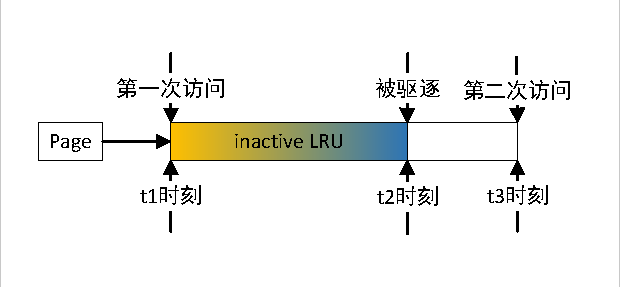
\includegraphics[width=0.5\textwidth]{重用距离.pdf}
  \caption{重用距离示意图}
  \label{fig:refault_distance}
\end{figure}

然而,在大型系统中为每个页面维护完整的访问信息以精确计算重用距离需要占用大量存储空间与数据结构维护开销。为此,我们借助近似策略:通过观察页面在活动链表(Active List)与非活动链表(Inactive List)间的迁移规律,来间接推断页面被访问的频度。当某页面在非活动链表上被替换(即被驱逐)后,若它在短期内再次被访问,即说明在此期间系统至少经历了一定数量的页面访问,从而可近似估计该页面的访问频率。


\subsection{重用距离的近似推导}

为了简化分析,先假设非活动链表长度固定,且暂不考虑活动链表向非活动链表的降级。这样可以更直观地专注于非活动链表上的页面替换与访问。图 \ref{fig:现象1} 与图 \ref{fig:现象2} 展示了两种核心场景。

\begin{figure}[htbp]
  \centering
  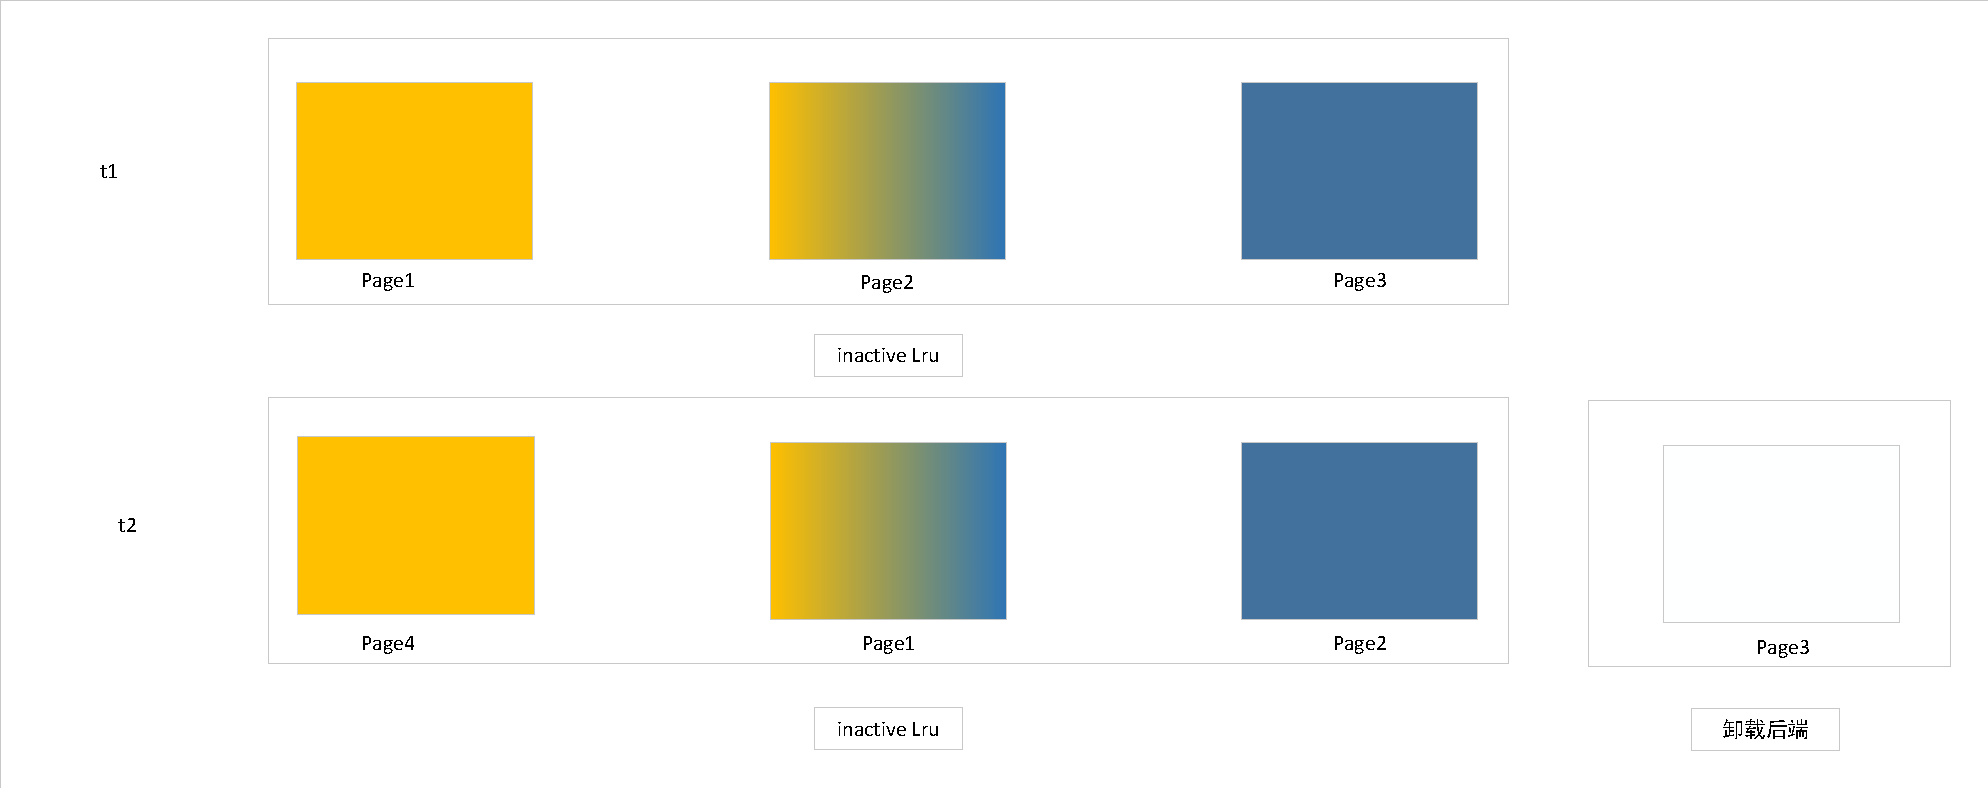
\includegraphics[width=0.5\textwidth]{现象1.pdf}
  \caption{情形一:页面首次插入非活动链表}
  \label{fig:现象1}
\end{figure}

\begin{figure}[htbp]
  \centering
  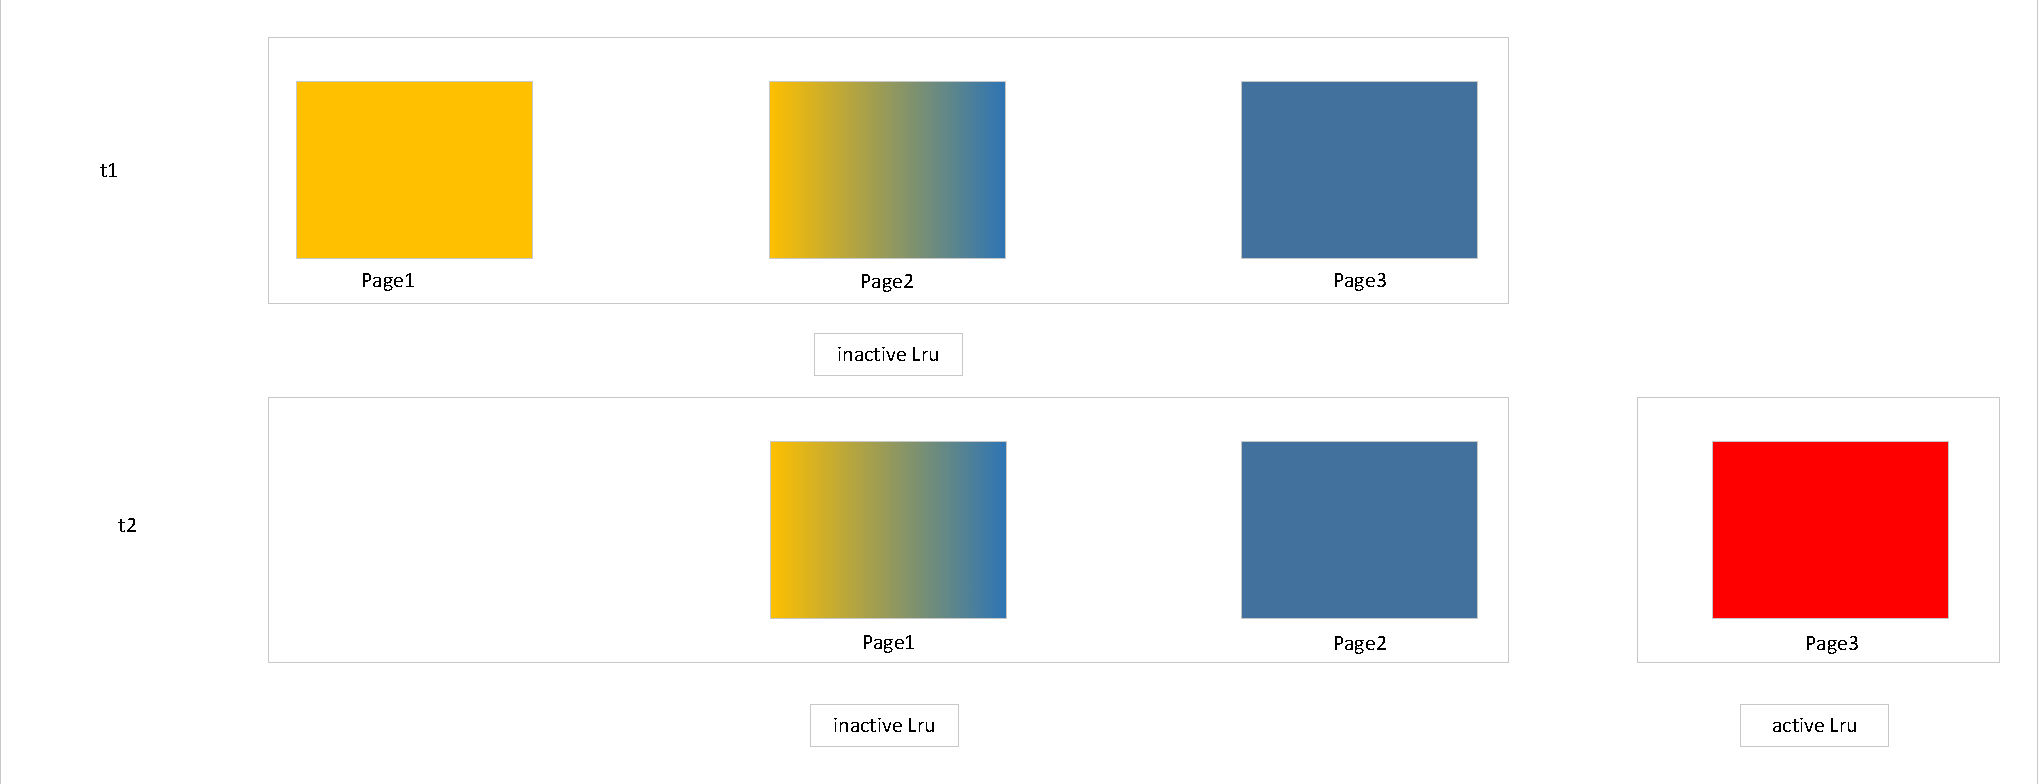
\includegraphics[width=0.5\textwidth]{现象2.pdf}
  \caption{情形二:页面在非活动链表上再次被访问并提升到活动链表}
  \label{fig:现象2}
\end{figure}

\noindent
\textbf{情形一}(图 \ref{fig:现象1})描述页面首次被访问并插入到非活动链表头部;由于链表长度固定,原链表中的页面整体向尾部滑动,最末尾页面被挤出内存(驱逐)。  
\textbf{情形二}(图 \ref{fig:现象2})描述页面在非活动链表上再次被访问后,被“提升”到活动链表,链表长度相应缩短;与此同时,所有比被提升页面更晚进入非活动链表的页面向尾部滑动,离被驱逐更近。

在时间区间 \([t_1, t_2]\) 内,非活动链表上的页面要么被驱逐(表明至少加载了新的页面),要么被提升至活动链表(表明被再次访问)。令
\[
  E(t_1,t_2)
\]
表示该区间内的驱逐次数(evictions),令
\[
  A(t_1,t_2)
\]
表示该区间的页面提升次数(activations)。因为每次驱逐对应至少一次新页面的载入,每次提升对应至少一次对非活动链表中页面的访问,故可以近似认为 \([t_1,t_2]\) 时间段内发生的最少页面访问数不低于
\begin{align}
  \label{eq:e_plus_a}
  E(t_1,t_2) \;+\; A(t_1,t_2).
\end{align}
真实系统中还需考虑一直停留在活动链表、从未降级的页面访问量。不过,对访问极频繁的页面而言,由于它们并不进入非活动链表,我们无需担心其“再次访问”情形的遗漏,因此对这部分页面的统计影响相对有限。


当页面 \(p\) 被驱逐时,我们记录其驱逐时刻 \(t_1\) 对应的计数器 \(\mathrm{count}(t_1)\),该计数器反映系统自启动至 \(t_1\) 时刻产生的驱逐次数与提升次数之和。

若该页面于时刻 \(t_2\) 再次被访问,则同样记录 \(count(t_2)\)。此时,我们定义页面 \(p\) 的重新故障距离(Refault Distance)为
\begin{align}
  \label{eq:refault_distance}
  D_{\mathrm{refault}}(p)
  &= 
  \mathrm{count}(t_2)
  \;-\;
  \mathrm{count}(t_1).
\end{align}
这一距离衡量了页面从被驱逐到再次访问期间,系统所经历的最少页面访问次数。



我们使用非活动链表长度来近似页面在缓冲中的访问页面的个数,因为相当于他从非活动链表的头部移动到尾部,每次移动代表一个页面被访问。我们使用\( L_{inactive}\) 表示非活动链表长度。则可得到页面 \(p\) 的总“访问距离”近似形式:
\begin{align}
  \label{eq:dtotal}
  D_{\mathrm{total}}(p)
  &= 
  L_{\mathrm{inactive}}
  \;+\;
  \bigl(\mathrm{count}(t_2) \;-\; \mathrm{count}(t_1)\bigr).
\end{align}
若非活动链表长度较小且页面容易被迅速驱逐,则此段时间内计数器增量 \(\mathrm{count}(t_2)-\mathrm{count}(t_1)\) 较大,意味着更多访问量发生,也暗示着若页面不具备足够高的访问频率,就难以在非活动链表中维持。


\subsection{替换决策与回收策略}

结合活动链表长度 \(\displaystyle L_{\mathrm{active}}\) 进行分析,若希望页面继续留在内存中,则需要满足
\begin{align}
  \label{eq:active_condition}
  L_{\mathrm{inactive}}
  \;+\;
  \bigl(\mathrm{count}(t_2) \;-\; \mathrm{count}(t_1)\bigr)
  &\;\;\le\;\;
  L_{\mathrm{inactive}}
  \;+\;
  L_{\mathrm{active}},
\end{align}
化简后即
\[
  \mathrm{count}(t_2) - \mathrm{count}(t_1)
  \;\le\;
  L_{\mathrm{active}}.
\]
由此可知,当页面的重新故障距离不超过活动链表大小时,该页面的访问频度足以支撑其继续驻留在内存,避免被替换。

在实际应用中,我们亦可将此方法与操作系统中的 \(\mathrm{swappiness}\) 等参数结合,动态调整文件页与匿名页的回收策略。例如,
\begin{align}
  \mathrm{swappiness}
  &=
  \min\!
  \Bigl(
    \mathrm{swappiness}
    \,\times\,
    \bigl(1 \,+\, \mathrm{refault\_active}\bigr),
    \;150
  \Bigr),
\end{align}
其中 \(\mathrm{refault\_active}\) 代表在近一段时间内页面重新故障的比例,通过该值对回收过程进行调节。当系统检测到高频率的重新故障时,可以加大对某类页面的保护力度,减少不必要的回收动作;反之亦然。

综上,利用驱逐与提升次数近似统计页面访问情况,能在保持较低开销的同时,根据重用距离或重新故障距离来指导页面替换决策。此方法对于识别和保留热页面、及时回收冷页面具有实践价值,也为优化文件页与匿名页的回收比例提供了可行途径,在实际系统中可有效提升内存使用效率及整体性能。



% \subsection{冷热页面优化实现}

% \ref{sec:冷热页面优化}介绍了算法,根据算法我们需要以下数据:

% \begin{enumerate}
%     \item 全局的驱逐和提升次数之和
%     \item 上次refault次数之和
%     \item refault之和
%     \item 每个文件页面被驱逐时候的驱逐和提升次数之和
% \end{enumerate}

% 其中1,2,3可以在 lruvec 中使用原子全局变量实现,每次在驱逐页面和提升页面的时候我们直接使用原子操作增加计数就可以了。在每次接在的时候,判断如果\(
%   \mathrm{count}(t_2) - \mathrm{count}(t_1)
%   \;\le\;
%   L_{\mathrm{active}}.
% \) 则将refault次数之和加一。

% 但是最后一个需要记录每一个文件页面,这个是比较困难的。我们巧妙复用了page cache的槽,之前的page cache使用的是前缀树,索引是文件的偏移,值是struct page。现在我们直接使用page cache的原来的的槽来存储每个文件页被驱逐时候的驱逐和提升次数之和。但是这样也引来了问题,就是前缀树的结构不会自动回收,所以我们要使用shrink机制来回收。

% 下面我们将详细介绍。

% 关键是我们需要记录驱逐次数和提升次数,然后计算重用距离,然后根据重用距离和swappiness 来决定文件页和匿名页的回收比例。

% \subsubsection{重用距离实现}

% 我们在lruvec这个数据结构中,添加了三个成员,一个是驱逐次数和提升次数之和,一个是refault次数之和,一个是refault之和。

% \begin{table}[htbp]
%     \centering
%     \caption{lruvec结构体成员}
%     \label{tab:lruvec_struct}
%     \begin{tabular}{ccc}
%         \toprule
%         \textbf{成员} & \textbf{类型} & \textbf{说明} \\
%         \midrule
%         nr\_count & atomic\_long\_t & 驱逐次数和提升次数之和 \\
%         \midrule
%         nr\_refault\_last & atomic\_long\_t & 上次refault次数之和 \\
%         \midrule
%         nr\_refault & atomic\_long\_t & refault之和 \\
%         \bottomrule
%     \end{tabular}
% \end{table}

% nr\_count 是驱逐次数和提升次数之和,由于struct page需要 16字节对齐,所以最后他的地址的最后4位是0,所以我们可以用于存储标志位。并且内核已经提供好了框架,这些条目被称作异常条目,在每次访问的时候自动去判断,如果是00就是指针,直接使用。如果不是指针,则有框架处理。 
% % https://elixir.bootlin.com/linux/v4.14.327/source/include/linux/radix-tree.h#L49


% % /*
% %  * The bottom two bits of the slot determine how the remaining bits in the
% %  * slot are interpreted:
% %  *
% %  * 00 - data pointer
% %  * 01 - internal entry
% %  * 10 - exceptional entry
% %  * 11 - this bit combination is currently unused/reserved
% %  *
% %  * The internal entry may be a pointer to the next level in the tree, a
% %  * sibling entry, or an indicator that the entry in this slot has been moved
% %  * to another location in the tree and the lookup should be restarted.  While
% %  * NULL fits the 'data pointer' pattern, it means that there is no entry in
% %  * the tree for this index (no matter what level of the tree it is found at).
% %  * This means that you cannot store NULL in the tree as a value for the index.
% %  */
% % #define RADIX_TREE_ENTRY_MASK		3UL
% % #define RADIX_TREE_INTERNAL_NODE	1UL

% % /*
% %  * Most users of the radix tree store pointers but shmem/tmpfs stores swap
% %  * entries in the same tree.  They are marked as exceptional entries to
% %  * distinguish them from pointers to struct page.
% %  * EXCEPTIONAL_ENTRY tests the bit, EXCEPTIONAL_SHIFT shifts content past it.
% %  */

% 00 对应的是指针
% 01 对应的是驱逐次数和提升次数之和

% 所以我们在\_\_remove\_mapping中添加逻辑,如果要驱逐的文件页面,我们将nr\_count值赋值到page的指针槽中,然后左移两位,然后和10进行或运算,然后赋值给page的指针槽。
% 将nr\_count的的值加一。

% 等到下次内核访问的时候,会自动去判断,如果是异常条目,则会左移两位,取出该页面被驱逐时候的驱逐次数和提升次数之和,去和nr\_count进行比较相减,然后去和active lRU的个数进行比较,如果小于active lRU的个数,则将该页面加入到active lRU中,否则加入到inactive lRU中,并且将nr\_refault加一,代表发生了文件页面的重新故障。

% \subsubsection{页面计数的实现}

% Linux中使用struct page这个数据结构来表示一个4kb的大小的物理页面,由于现在使用的内存很大,到了tb级别,所以page的数量很多,里面的数据成员需要精心设计。除此之外,由于page经常被访问,所以他被设置成16字节对齐,这为我们实现页面计数提供了方便。

% 由于被设计成16字节对齐,所以最后他的地址的最后4位是0,所以我们可以用于存储标志位。在linux中,已经有很多模块都已经使用了这些标志位,比如slub模块和tmpfs模块,所以我们也可以复用这个标志位。

% \begin{figure}[h]
%     \centering
%     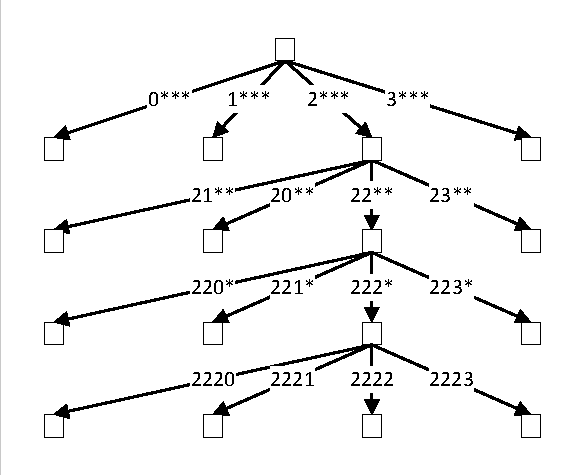
\includegraphics[width=\textwidth]{前缀树.pdf}
%     \caption{page cache的前缀树}
%     \label{fig:前缀树}
% \end{figure}

% 图片\ref{fig:前缀树}展示了page cache的前缀树结构,使用地址的中的几位作为索引,然后在最底层就是具体数据。 最底层每个节点表示一个文件的偏移,值是struct page的指针。但是我们可以复用后面2位,来存储标志位,Linux内核中也已经规定了,所以我们可以复用。



% \begin{table}[h]
%     \centering
%     \caption{标志位}
%     \label{tab:标志位}
%     \begin{tabular}{cc}
%         \toprule
%         \textbf{标志位} & \textbf{说明} \\
%         \midrule
%         00 & data pointer\\
%         \midrule
%         01 & internal entry\\
%         \midrule
%         10 & exceptional entry\\
%         \midrule
%         11 & this bit combination is currently unused/reserved\\
%         \bottomrule
%     \end{tabular}
% \end{table}

% 其中,我们使用文件页中的异常条目没有被使用,所以我们可以复用。

% \begin{figure}[h]
%     \centering
%     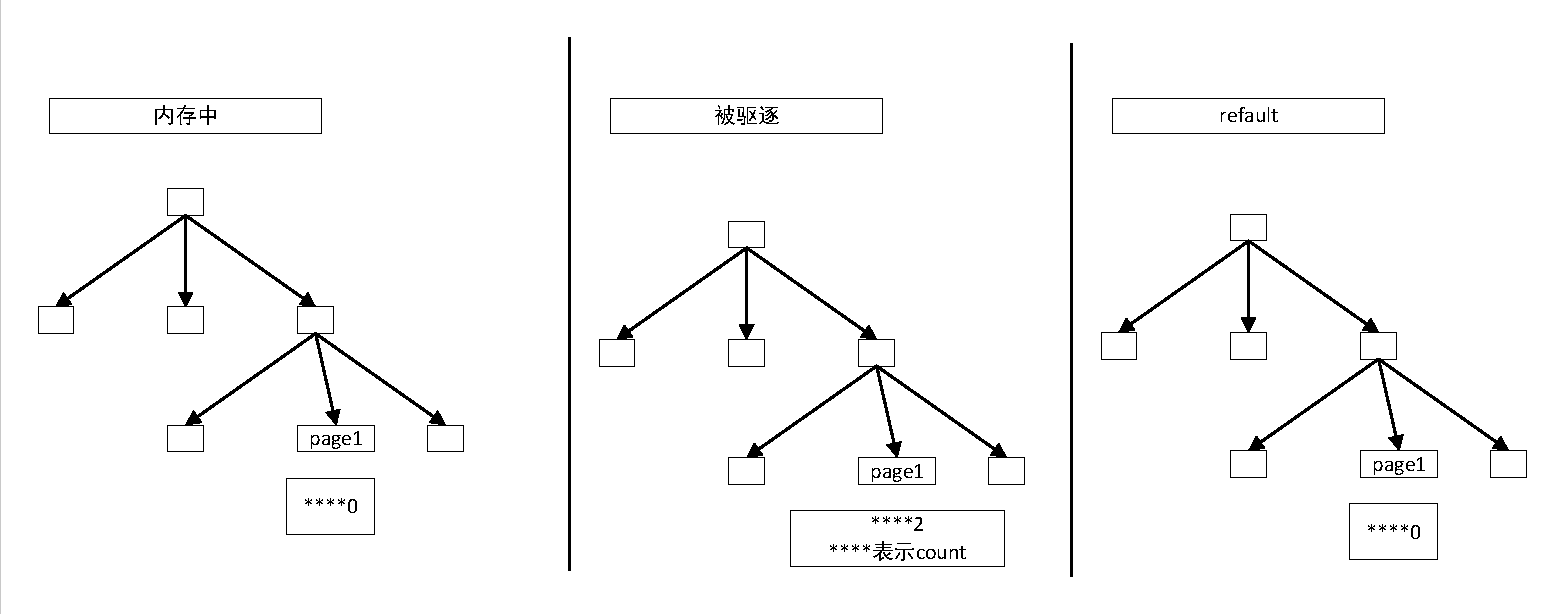
\includegraphics[width=\textwidth]{复用.pdf}
%     \caption{复用}
%     \label{fig:复用}
% \end{figure}

% 图片\ref{fig:复用}展示了复用的情况,当页面的在内存的时候,使用00表示指针,当页面被驱逐的时候,使用10表示异常条目。这种情况既不会导致错误的访问,也可以实现每个页面的计数,也需要需要大量的内存来管理。

% \subsubsection{Shrinker机制的工作原理}

% 由于我们复用了page cache中的条目,导致这部分条目不会被释放,所以需要使用Shrinker机制来释放。
% Linux内核中的Shrinker机制是内存回收子系统的重要组成部分,用于在系统内存压力增大时回收可释放的缓存对象。当系统内存不足时,页面回收进程会调用注册的shrinker回调函数来释放缓存,从而缓解内存压力。Shrinker机制主要应用于各类缓存系统,如inode缓存、dentry缓存和各种文件系统的专用缓存等。

% Shrinker机制在内核的页面回收路径中起作用,特别是在以下场景:
% \begin{itemize}
%     \item 直接内存回收(Direct Reclaim):当分配内存失败且允许等待时触发
%     \item kswapd内核线程:周期性检查内存状态,在内存压力大时主动回收
%     \item 内存紧急回收(Memory Cgroup Reclaim):当某个内存控制组超出限制时触发
% \end{itemize}

% \paragraph {核心数据结构分析}

% Shrinker机制主要涉及两个关键数据结构:\texttt{struct shrinker}和\texttt{struct shrink\_control}。

% \paragraph{shrink\_control结构体}

% \texttt{struct shrink\_control}用于在页面回收子系统和shrinker回调函数之间传递信息。\ref{tab:shrink_control_struct}详细说明了结构体的成员。

% \begin{table}[h]
% \label{tab:shrink_control_struct}
% \centering
% \begin{tabular}{ccc}
% \toprule
% \textbf{成员} & \textbf{类型} & \textbf{说明} \\
% \midrule
% gfp\_mask & gfp\_t & 当前内存分配的标志,指示分配的约束条件 \\
% \midrule
% nid & int & 当前正在进行内存回收的NUMA节点ID \\
% \midrule
% nr\_to\_scan & unsigned long & 指示scan\_objects应尝试回收的对象数量\\
% \midrule
% nr\_scanned & unsigned long & scan\_objects实际处理的对象数量,默认值为nr\_to\_scan \\
% \midrule
% memcg & struct mem\_cgroup * & 当前正在进行内存回收的memory cgroup \\
% \bottomrule
% \end{tabular}
% \caption{shrink\_control结构体成员说明}
% \end{table}

% \paragraph{shrinker结构体}

% \texttt{struct shrinker}定义了一个可注册的回调函数组,用于对可回收缓存施加压力。\ref{tab:shrinker_struct}详细说明了结构体的成员。

% \begin{table}[htbp]
% \label{tab:shrinker_struct}
% \centering
% \begin{tabular}{ccc}
% \toprule
% \textbf{成员} & \textbf{类型} & \textbf{说明} \\
% \midrule
% count\_objects & 函数指针 & 返回缓存中可释放对象的数量,若无可释放对象则返回SHRINK\_EMPTY,若无法确定或应跳过则返回0 \\
% \midrule
% scan\_objects & 函数指针 & 扫描缓存并尝试释放项目,返回已释放对象数量,若因潜在死锁无法继续则返回SHRINK\_STOP \\
% \midrule
% batch & long & 回收批次大小,0表示使用默认值 \\
% \midrule
% seeks & int & 重新创建一个对象所需的磁盘寻道次数,影响回收优先级 \\
% \midrule
% flags & unsigned & shrinker能力标志,如NUMA感知、memcg感知等 \\
% \midrule
% list & struct list\_head & 内部使用,用于将shrinker链接到全局列表 \\
% \midrule
% id & int & 在memcg\_kmem配置下使用的shrinker标识符 \\
% \midrule
% nr\_deferred & atomic\_long\_t * & 按节点统计的待删除对象,用于延迟处理 \\
% \bottomrule
% \end{tabular}
% \caption{shrinker结构体成员说明}
% \end{table}

% \paragraph{Shrinker的注册与使用}

% 内核提供了以下API用于注册和管理shrinker:

% \begin{itemize}
%     \item \texttt{prealloc\_shrinker()}:预分配shrinker相关资源
%     \item \texttt{register\_shrinker\_prepared()}:注册已预分配资源的shrinker
%     \item \texttt{register\_shrinker()}:注册新的shrinker
%     \item \texttt{unregister\_shrinker()}:注销已注册的shrinker
%     \item \texttt{free\_prealloced\_shrinker()}:释放预分配的shrinker资源
% \end{itemize}

% \paragraph{自定义Shrinker的实现方法}

% 要实现一个自定义的shrinker,需要完成以下步骤:

% 1. 定义shrinker结构体并实现必要的回调函数
% 2. 注册shrinker到内核
% 3. 在不再需要时注销shrinker

% Linux内核中的Shrinker机制为各类缓存系统提供了统一的内存回收接口,是内核内存管理的重要组成部分。通过实现count\_objects和scan\_objects回调函数,各子系统可以向内存回收子系统提供可回收对象的信息,并在内存压力下主动释放这些对象。这种机制既保证了内核在内存紧张时的稳定性,又保持了各缓存系统的独立性和灵活性。

\subsection{冷热页面优化的实现原理与机制}

前文的算法设计(\ref{sec:冷热页面优化})提出了基于重用距离(Reuse Distance)来优化冷热页面的思路。为在内核中落地该算法,需要在多个方面进行配合:首先是全局驱逐(eviction)和提升(activation)次数等计数的维护,其次是单个文件页面被驱逐时刻的计数存储,最后还需借助 Shrinker 机制回收不再使用的异常条目,从而保持系统稳定性。下面从整体到局部进行说明。

\subsection{核心计数数据与整体框架}

根据算法需求,我们至少需维护四类计数信息:
\begin{enumerate}
  \item 全局的驱逐和提升次数之和(后文以 \(\mathrm{nr\_count}\) 表示)。
  \item 上次重新故障(refault)统计的次数之和(\(\mathrm{nr\_refault\_last}\))。
  \item 当前时刻累积的重新故障次数之和(\(\mathrm{nr\_refault}\))。
  \item 文件页面被驱逐时对应的驱逐与提升次数之和(记录在页面自身或其关联结构中)。
\end{enumerate}

其中,前 3 项可直接存储在 \texttt{lruvec} 结构体的原子变量中,一旦页面产生驱逐或提升事件,即对 \(\mathrm{nr\_count}\) 执行原子加一。在页面再次加载时,如果满足
\[
  \mathrm{count}(t_2) \;-\; \mathrm{count}(t_1)
  \;\le\;
  L_{\mathrm{active}},
\]
则说明页面在被驱逐后并未经历太长时间就再次被访问,可视为一次重新故障(refault),并相应地增加 \(\mathrm{nr\_refault}\) 计数。

然而,第 4 项对“每个文件页面被驱逐时的计数值”提出了额外要求:需要在页与文件偏移关联的 \texttt{page cache} 中进行记录,且在页面再次载入时还能恢复该计数用于比较。下文详述了如何在 \texttt{page cache} 的前缀树中复用现有结构完成此操作。

\begin{table}[htbp]
  \centering
  \caption{\texttt{lruvec} 结构体中新增的核心成员}
  \label{tab:lruvec_struct}
  \begin{tabular}{ccc}
    \toprule
    \textbf{成员} & \textbf{类型} & \textbf{说明} \\
    \midrule
    \(\mathrm{nr\_count}\) & \texttt{atomic\_long\_t} & 全局驱逐次数与提升次数之和 \\
    \midrule
    \(\mathrm{nr\_refault\_last}\) & \texttt{atomic\_long\_t} & 上次统计时的 refault 次数之和 \\
    \midrule
    \(\mathrm{nr\_refault}\) & \texttt{atomic\_long\_t} & 当前 refault 次数之和 \\
    \bottomrule
  \end{tabular}
\end{table}

\subsubsection{基于异常条目的重用距离记录}

\paragraph{前缀树与异常条目的复用}

Linux 内核中 \texttt{page cache} 的索引结构通常使用前缀树(Radix Tree),底层将文件偏移映射到 \texttt{struct page} 指针。图\ref{fig:前缀树}展示了page cache的前缀树结构,其中每个节点表示一个文件的偏移,值是struct page的指针。

为了实现“页面被驱逐时记下全局计数”的需求,我们复用该指针槽的标志位。  
由于 \texttt{struct page} 对齐方式通常为 16 字节,其指针低位保留 2 位作为标识(\texttt{00}, \texttt{01}, \texttt{10}, \texttt{11}),内核已定义了相应宏来区分“正常指针”、“内部节点”以及“异常条目”等。下表与图示展示了此机制。

\begin{table}[htbp]
  \centering
  \caption{标志位含义与用途}
  \label{tab:标志位}
  \begin{tabular}{cc}
    \toprule
    \textbf{标志位} & \textbf{说明} \\
    \midrule
    \texttt{00} & 指向 \texttt{struct page} 的正常指针 \\
    \texttt{01} & 内部节点 \\
    \texttt{10} & 异常条目(exceptional entry) \\
    \texttt{11} & 目前保留未用 \\
    \bottomrule
  \end{tabular}
\end{table}

\begin{figure}[htbp]
  \centering
  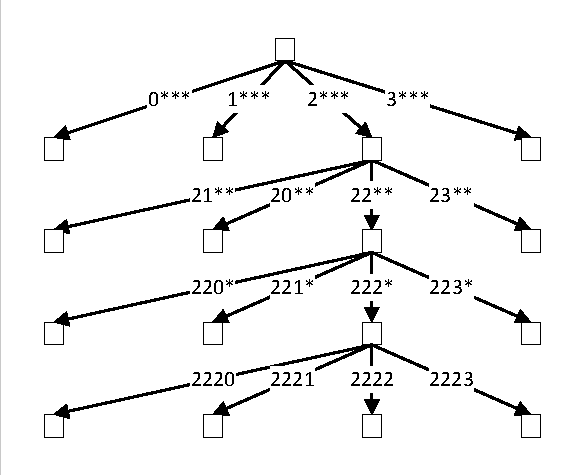
\includegraphics[width=\textwidth]{前缀树.pdf}
  \caption{\texttt{page cache} 的前缀树结构示意}
  \label{fig:前缀树}
\end{figure}

\paragraph{驱逐与再加载时的数据流转}
当某文件页面即将被驱逐(在 \texttt{\_\_remove\_mapping} 中):
\begin{enumerate}
  \item 读取当前 \(\mathrm{nr\_count}\) 原子计数,并将其左移 2 位(为标志位留出空间)。
  \item 与 \(\texttt{10}\) 做或运算,生成“异常条目”,写回前缀树对应索引槽。
  \item 对全局 \(\mathrm{nr\_count}\) 加一,表示发生了一次新的驱逐事件。
  \item 从系统的活动或非活动链表中正式移除该页面,完成驱逐。
\end{enumerate}

当后续对同一文件偏移发生缺页中断(page fault)而需要载入页面时:
\begin{enumerate}
  \item 内核检测到该索引槽存储的标识位并非 \texttt{00}(正常指针),判断其为异常条目。
  \item 提取异常条目中的数值并右移 2 位得到页面被驱逐时的 \(\mathrm{nr\_count}\)。
  \item 计算 \(\mathrm{nr\_count}(t_2) - \mathrm{nr\_count}(t_1)\),若结果不超过活动链表长度 \(L_{\mathrm{active}}\),则视为短期内再访问,此时提升该页面至活动链表,并增大 \(\mathrm{nr\_refault}\) 计数。
  \item 若超出阈值,则仅将该页面放入非活动链表观察,无需更新 \(\mathrm{nr\_refault}\)。
\end{enumerate}

\begin{figure}[htbp]
  \centering
  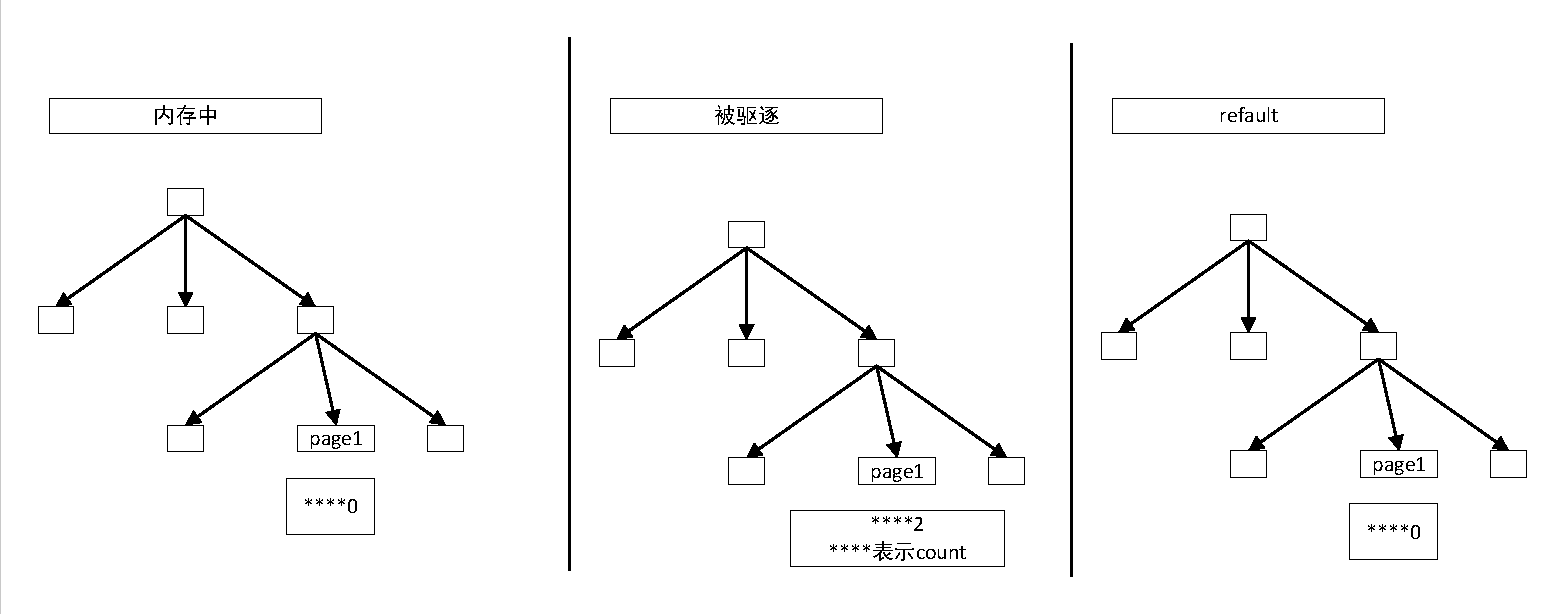
\includegraphics[width=\textwidth]{复用.pdf}
  \caption{利用异常条目存储驱逐时的 \(\mathrm{nr\_count}\)}
  \label{fig:复用}
\end{figure}

如图 \ref{fig:复用} 所示,页面在内存中时使用普通指针(标志位 \texttt{00});被驱逐后则切换为异常条目(标志位 \texttt{10});再加载时可根据此信息计算重用距离并作相应处理。该方法避免了在 \texttt{struct page} 内部额外存储驱逐计数,最大化复用内核已有数据结构。

\subsubsection{Shrinker 机制:缓存回收与资源释放}

\paragraph{为什么需要 Shrinker}

将驱逐过的页面“异常条目”保留在 \texttt{page cache} 的前缀树中,会导致索引节点数量不断累积,若不加以限制,可能造成内存浪费。此时就需要 Shrinker 机制在内存紧张时主动清理这些不再需要的异常条目。

\paragraph{Shrinker 机制概览}

Shrinker 是 Linux 内核内存回收子系统(MM Subsystem)中的统一回调接口,用于管理诸如 inode、dentry 以及各种自定义缓存。内核在以下场景可能触发 Shrinker:
\begin{itemize}
  \item \textbf{直接内存回收(Direct Reclaim)}:进程分配内存失败后尝试同步回收。
  \item \textbf{后台回收线程(kswapd)}:周期性检查系统内存使用情况,在紧张时主动回收。
  \item \textbf{Memory Cgroup 回收(Memcg Reclaim)}:当某内存控制组超出其配额时触发。
\end{itemize}
Shrinker 通过 \texttt{struct shrink\_control}(表 \ref{tab:shrink_control_struct})与 \texttt{struct shrinker}(表 \ref{tab:shrinker_struct})两个核心数据结构向回收框架注册接口,内核则在内存压力情形下调用对应的回调函数执行清理动作。

\begin{table}[htbp]
  \centering
  \caption{\texttt{shrink\_control} 结构体主要字段说明}
  \label{tab:shrink_control_struct}
  \begin{tabular}{ccc}
    \toprule
    \textbf{成员} & \textbf{类型} & \textbf{说明} \\
    \midrule
    \texttt{gfp\_mask} & \texttt{gfp\_t} & 本次内存分配的掩码,指示约束条件 \\
    \texttt{nid} & \texttt{int} & 所在的 NUMA 节点 \\
    \texttt{nr\_to\_scan} & \texttt{unsigned long} & 期望本轮扫描并回收的对象数 \\
    \texttt{nr\_scanned} & \texttt{unsigned long} & 实际扫描对象数量 \\
    \texttt{memcg} & \texttt{struct mem\_cgroup *} & 针对特定 \texttt{memcg} 的回收(若有) \\
    \bottomrule
  \end{tabular}
\end{table}

\begin{table}[htbp]
  \centering
  \caption{\texttt{struct shrinker} 结构体主要字段说明}
  \label{tab:shrinker_struct}
  \begin{tabular}{ccc}
    \toprule
    \textbf{成员} & \textbf{类型} & \textbf{说明} \\
    \midrule
    \texttt{count\_objects} & 函数指针 & 返回可回收对象数,若无可回收则 \texttt{SHRINK\_EMPTY} \\
    \texttt{scan\_objects} & 函数指针 & 实际扫描并回收对象,返回已释放数量 \\
    \texttt{batch} & \texttt{long} & 每次回收的批次大小,默认为 0(使用默认值) \\
    \texttt{seeks} & \texttt{int} & 反映对象重建开销,影响回收优先级 \\
    \texttt{flags} & \texttt{unsigned} & Shrinker 能力标志(NUMA 感知等) \\
    \texttt{list} & \texttt{struct list\_head} & 内核内部使用,用于将 shrinker 链接到全局列表 \\
    \texttt{id} & \texttt{int} & 在 memcg 上下文中的 shrinker 标识 \\
    \texttt{nr\_deferred} & \texttt{atomic\_long\_t *} & 延迟对象数计数 \\
    \bottomrule
  \end{tabular}
\end{table}

\paragraph{自定义 Shrinker 回调的编写}

为释放不再使用的异常条目,需要:
\begin{enumerate}
  \item \textbf{定义 \texttt{struct shrinker} 结构},实现
  \begin{itemize}
    \item \texttt{count\_objects}:返回“可释放异常条目”数量。
    \item \texttt{scan\_objects}:对前缀树节点执行实际回收操作,将长时间未使用的异常条目清理掉。
  \end{itemize}
  \item \textbf{注册 \texttt{shrinker}}:通过 \texttt{register\_shrinker()} 或相关接口将其加入内核回收体系。
  \item \textbf{在不需要时注销 \texttt{shrinker}}:如模块卸载或场景切换时,调用 \texttt{unregister\_shrinker()}。
\end{enumerate}

Shrinker 回调需结合系统内存状态、访问统计等信息,以避免在正常负载时盲目回收、增加额外开销。同时,需确保不会在回收函数中发生较大锁争用或再次触发内存分配,避免死锁等问题。

\subsubsection{总结与展望}

综上所述,本节介绍了冷热页面优化在内核中的具体实现路径:利用 \texttt{lruvec} 中的全局计数器统计驱逐/提升事件,借助异常条目在 \texttt{page cache} 中为每个文件页记录被驱逐时刻的计数值,并通过 Shrinker 机制定期回收冗余异常条目,从而在系统层面有效识别并保留热页面、及时回收冷页面。  
该方法无需额外扩展 \texttt{struct page} 结构即可实现重用距离的近似估算,对大规模服务器和高负载环境具备良好的可扩展性。未来工作可结合多 NUMA 节点访问模式,或针对匿名页面与文件页面配置差异化的回收策略,以进一步提升内存管理的整体效率与性能。


\chapter{实验测试与结果分析}

\section{实验环境与测试负载}

\subsection{硬件配置}

\subsection{实验环境选择说明}

本研究涉及对Linux内核的深度修改与定制,实验环境的选择受到多种因素的限制。首先,由于对内核进行了大量底层改动,测试环境需要完全控制系统底层权限并能够频繁重启以更新内核,而生产环境不允许此类操作;其次,修改后的内核需要经过充分验证才能部署到高端服务器上,以避免潜在的系统稳定性问题。因此,本研究采用了性能较为有限的笔记本电脑作为测试平台,虽然测试平台的绝对性能与企业级服务器存在差距,但本研究关注的是不同算法间的相对性能比较,以及算法在不同工作负载下的适应性表现,这些方面的结论在很大程度上可以推广到更高性能的硬件环境中。未来研究中,在核心算法稳定后,可考虑在大规模服务器集群上进行进一步验证。

表\ref{tab:hardware_config}汇总了实验平台的具体配置,可以看到该平台拥有 Intel(R) Core(TM) i7-8750H CPU @ 2.20GHz 以及 16GB DDR4 内存。为了在内核中进行对比,本研究分别选取了机械硬盘、SSD 和 zram 这三种不同的卸载后端。之所以进行这样的选择,一方面是由于官方内核暂未实现基于 RDMA 和 NVM 的卸载后端,另一方面也是为了更好地体现不同存储介质在 I/O 延迟和读写性能方面的差异。机械硬盘能够代表最传统、也是性能相对最差的卸载方式,SSD 在随机读写和延迟方面有一定程度提升,而 zram 则具有数据压缩和低延迟的优势,通常被认为是内存交换的优先方案。为了凸显 zram 的潜在优势,并评估自适应算法在高压缩比数据下的实际效果,本文在后续测试中也将 zram 视为可获得最优 I/O 性能的后端加以重点分析。

\begin{table}[ht]
    \centering
    \caption{实验平台硬件配置}
    \label{tab:hardware_config}
    \begin{tabular}{ll}
        \toprule
        CPU & Intel(R) Core(TM) i7-8750H @ 2.20GHz \\
        \midrule
        Memory & 16GB (2 \(\times\) 8GB) DDR4 @ 2667MT/s SODIMM \\
        \midrule
        SSD & Intel SSDPEKKW256G8 NVMe SSD (256GB, PCIe Gen3 x4)  \\
        \midrule
        HDD & Seagate ST1000LM035 HDD (1TB, 5400 RPM) \\
        \bottomrule
    \end{tabular}
\end{table}

在负载选择方面,为了更全面地测试本文提出方案的通用性,实验分别使用了文件密集型的 Web Server 和内存密集型的 Redis 这两类典型应用。Web Server 场景主要用于观察系统针对大量静态文件(包括高清图片与文本数据)缓存时的文件页回收策略,而 Redis 场景则聚焦在匿名页占比极高的内存回收状态。值得注意的是,在 Redis 测试中禁止了持久化功能并关闭了淘汰策略,这样能更直接地暴露内存回收在内核层面的有效性,因为一旦允许用户态自行管理持久化或淘汰,就会在应用层与内核层产生额外耦合,从而干扰对回收策略的评估。

\section{模块功能与有效性测试}

\subsection{内存压力模块有效性验证}

在展开具体算法评估之前,需要首先验证所设计的内存压力模块能否在不借助用户态复杂逻辑的前提下,为系统施加可量化的内存压力。为此,本文使用了 Web Server 作为负载,将各种类型的图片和文字文件提前放入服务器端,随后利用压力发生器随机并持续地发起请求,同时在内核中分别配置机械硬盘、SSD 和 zram 作为卸载后端。通过这样的方式,可以从 16GB 可用内存开始,逐步减少可用空间直到 6GB,借此形成多轮测试,并观察在不同后端介质下系统对内存压力的响应程度。图\ref{fig:memory_pressure}展示了三种卸载后端下的内存压力曲线。可以明显看出,机械硬盘由于读写延迟和带宽的劣势,会更频繁地陷入换入换出操作,导致系统大量时间都处在高压力区间,甚至难以稳定地对外提供请求服务;相比之下,SSD 提供了更快的 I/O 响应能力,zram 在具有压缩和低访问延迟的双重优势下,则能进一步缓解内存压力飙升的问题。通过该实验可以确认本研究的内存压力模块在不同后端下均能触发与还原高压场景所需的换页流程,且能够准确地量化系统内存使用状况,为后续的自适应回收算法测试奠定基础。

\begin{figure}[htbp]
    \centering
    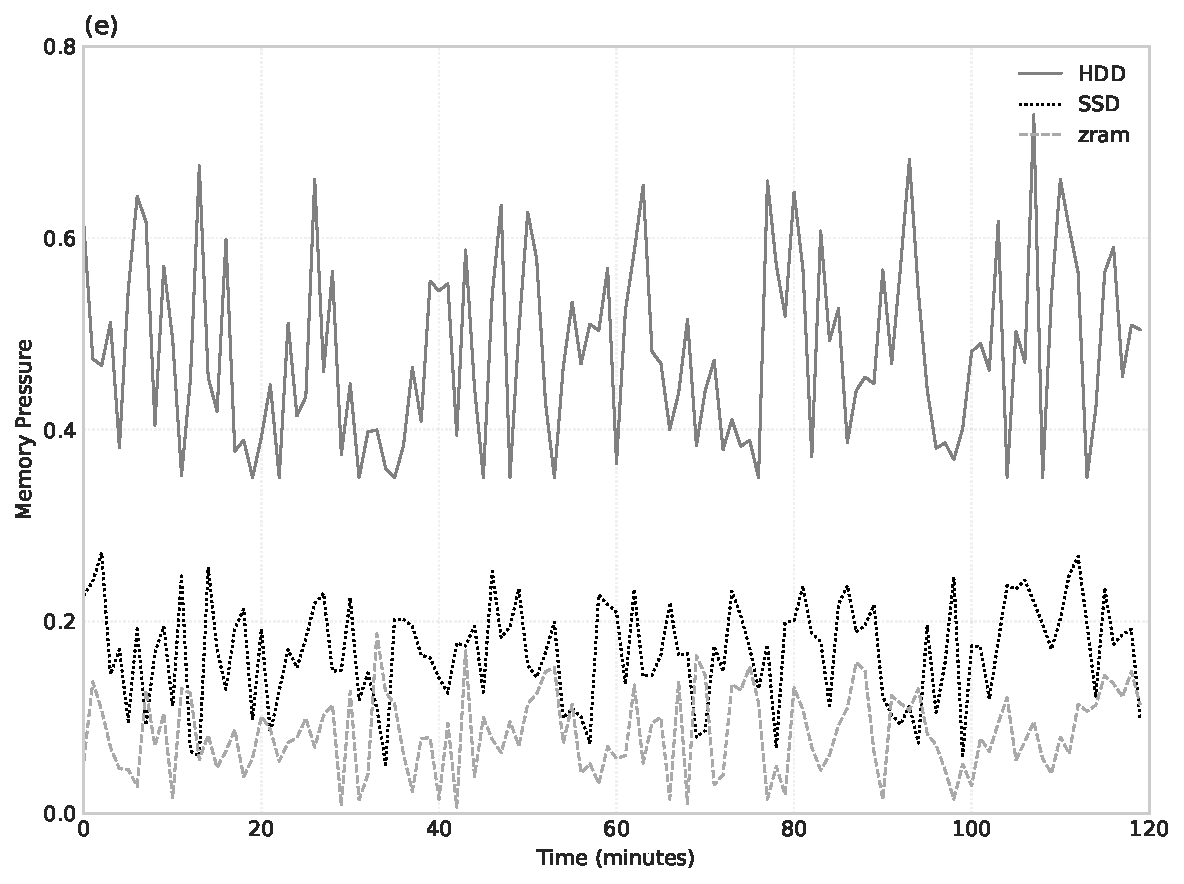
\includegraphics[width=\textwidth]{memory_pressure.pdf}
    \caption{三种卸载后端下的内存压力对比}
    \label{fig:memory_pressure}
\end{figure}


\subsection{文件页与匿名页均衡算法有效性验证}
\label{sec:file_page_anonymous_page_balance_algorithm_validation}

在确认内存压力模块可以生成可控且真实的压力环境后,需要检验自适应回收算法的第二个核心:即针对文件页与匿名页的均衡回收机制。为此,本文选取了 10GB 的可用内存作为上限来运行高负载场景,并针对 Linux 内核中的 \texttt{swappiness} 参数进行多轮对比测试。实验中分别测试了使用默认内核策略(baseline)和启用自适应均衡算法(adaptive  swappiness)两种情况下的系统性能表现。

\begin{figure}[htbp]
    \centering
    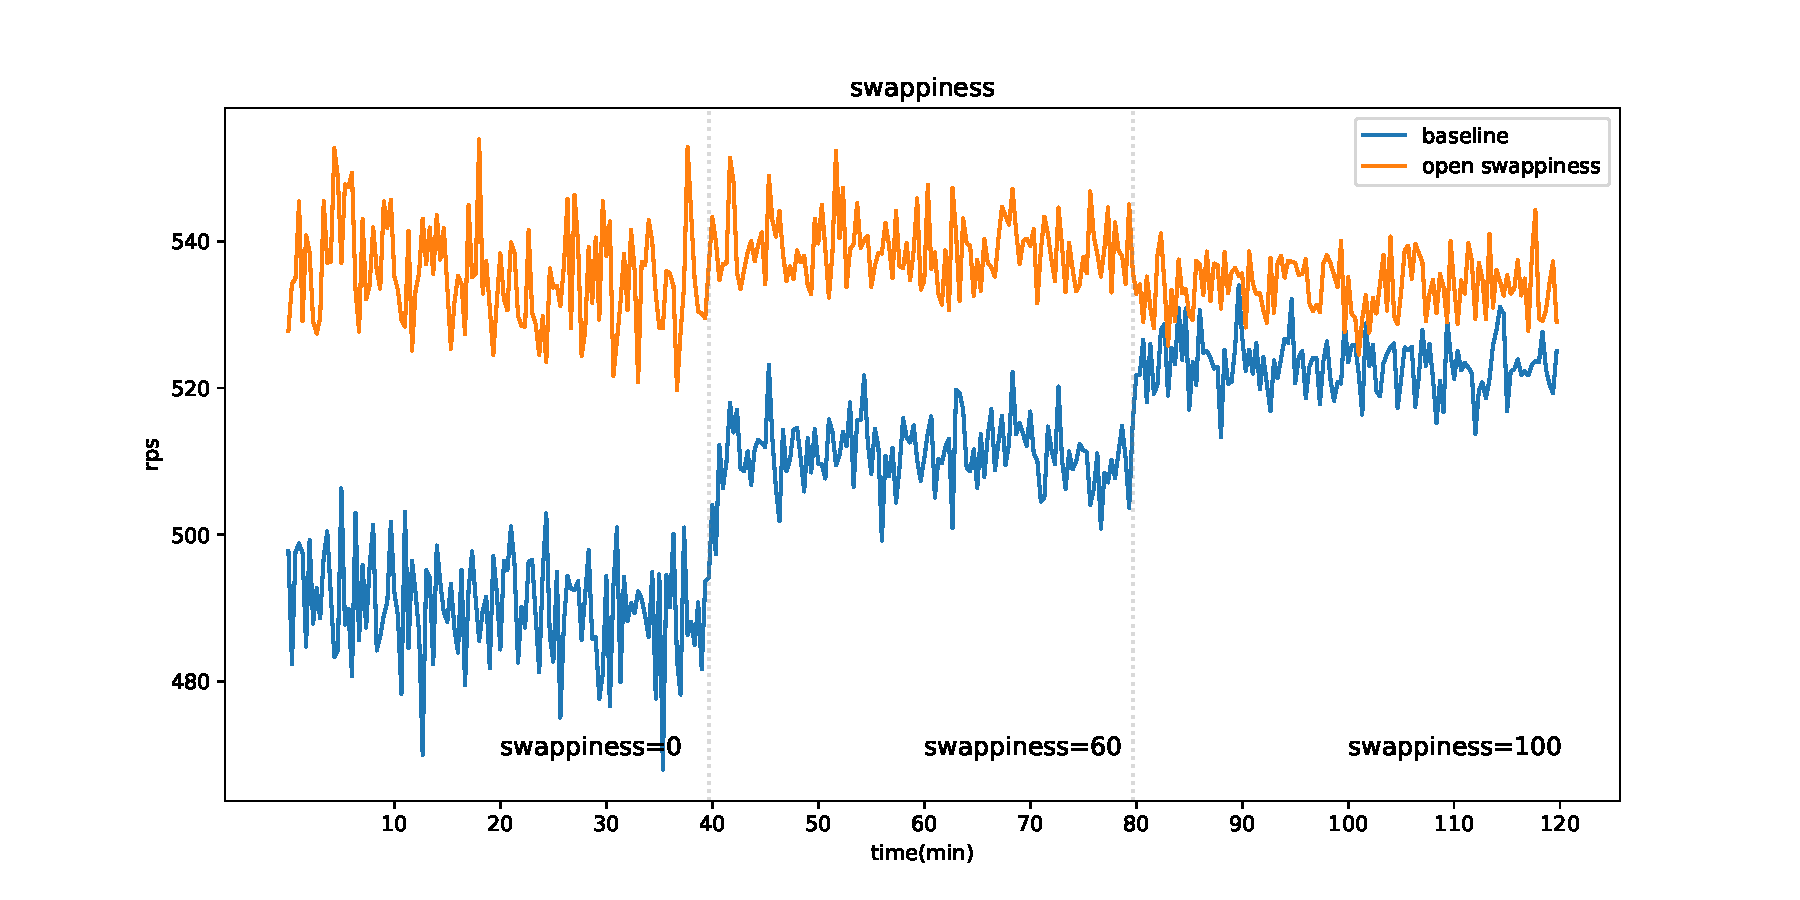
\includegraphics[width=\textwidth]{swappiness.pdf}
    \caption{Web Server 在不同 \texttt{swappiness} 下的性能变化}
    \label{fig:web_server_swappiness}
\end{figure}

首先在文件密集型负载(Web Server)下进行测试,如图\ref{fig:web_server_swappiness}所示。在默认内核策略下,当 \texttt{swappiness}=0 时,系统优先回收文件页而保留匿名页,导致Web Server所需的文件缓存被频繁驱逐,平均RPS仅维持在490左右;当 \texttt{swappiness} 提升至 60 时,系统开始更均衡地回收文件页和匿名页,使得Web Server的关键文件缓存得到一定保留,RPS明显提升至约515;进一步将\texttt{swappiness}提高到100时,RPS继续小幅上升至520左右,但增幅已不显著,这表明在文件密集型负载下,适当提高匿名页回收比例能有效改善系统性能。

当启用自适应均衡算法后,其性能表现更为优异。图中橙色曲线显示,无论\texttt{swappiness}设置为何值,系统吞吐量均维持在535-540之间的较高水平,且波动较小。特别是在\texttt{swappiness}=0的情况下,相比默认策略提升了约10\%的吞吐量,这证明了算法能够准确识别频繁访问的文件页,并通过动态调整回收策略避免了过度驱逐热文件页的问题。

\begin{figure}[htbp]
    \centering
    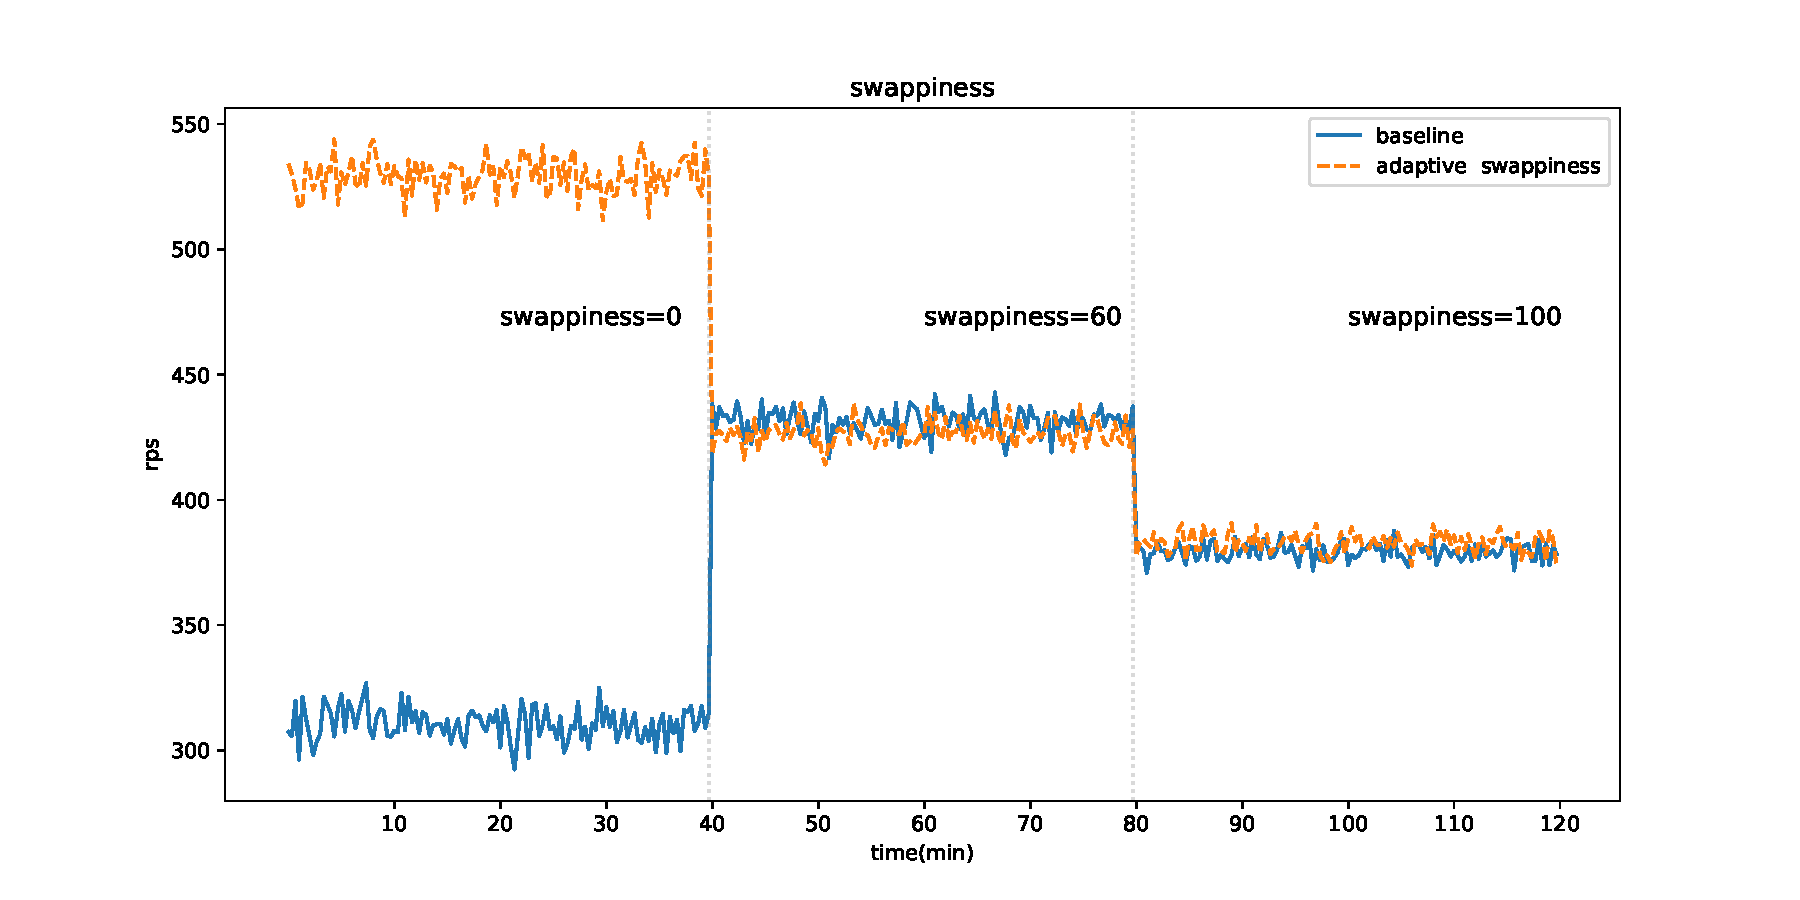
\includegraphics[width=\textwidth]{redis_swappiness.pdf}
    \caption{Redis 在不同 \texttt{swappiness} 下的性能变化}
    \label{fig:redis_swappiness}
\end{figure}

为验证算法在不同类型工作负载下的适应性,本文进一步选取了Redis作为内存密集型测试对象。如图\ref{fig:redis_swappiness}所示,Redis测试展现出了与Web Server截然不同的性能特征。在默认内核策略下,\texttt{swappiness}=0时Redis的平均RPS仅为310左右;当提高至\texttt{swappiness}=60后,RPS骤增至430左右;而进一步提高至\texttt{swappiness}=100时,性能又下降至380左右。这一曲线变化表明,在匿名页占主导的Redis工作负载中,过低的\texttt{swappiness}值会导致系统几乎不回收匿名页,使得内存压力集中在文件页上,而这些文件页可能包含程序代码等关键部分;适度提高\texttt{swappiness}可以实现更均衡的回收策略;但过高的值则会导致过度回收匿名页,引发频繁的页面换入换出。

当启用自适应均衡算法后,系统表现出更强的环境适应能力。在\texttt{swappiness}为0的配置下,启用算法的Redis性能(约525 RPS)显著优于默认策略,远高于任何\texttt{swappiness}值下的默认策略表现。这表明算法能够通过分析页面访问模式,自动调整回收策略,避免了在内存紧张时对程序关键文件页的错误驱逐。在\texttt{swappiness}=60和100的配置下,启用算法后的性能与默认策略相近,这是因为在Redis这类匿名页占比极高(约90\%)的场景中,文件页缺页率相对较低,算法优化空间有限。

实验结果表明,本文提出的文件页与匿名页均衡算法在不同类型的工作负载下均能展现良好适应性。在文件密集型负载中,算法能够通过精确识别热文件页并保留它们来提升性能;在内存密集型负载中,算法也能避免关键文件页被错误驱逐。虽然在极高匿名页占比的环境中算法的优化空间相对有限,但这也符合内存管理的理论预期,因为当工作集几乎完全由匿名页构成时,页面类型差异化回收的影响自然会降低。通过这两类代表性应用的实验,初步验证了该算法具有较强的通用适应能力。

\section{综合测试}

\subsection{测试目标}

上述实验分别验证了内存压力模块在不同后端介质下的量化能力,以及文件页与匿名页均衡算法在不同类型工作负载下的适应性。为了更深入地了解将二者结合起来后对系统整体性能和资源使用的影响,本文设计了综合测试。该测试主要聚焦以下问题:在持续提供服务的高负载场景下,若开启自适应算法并在不同后端(SSD 与 zram)进行内存卸载,系统能否稳定提升吞吐量并节约内存占用;在用户态应用(如 Web Server)长期占用大规模文件页以及针对容器化的多进程场景下,算法是否依旧有良好的适应性。

\subsection{测试方案}

首先在 Web Server 场景下,通过一轮预热请求将常见的文件页面基本加载至内存中,以形成完整的工作集,然后维持高并发请求并逐步向系统注入额外的内存压力,依次在以下场景下进行对比:(1) 禁用 \texttt{swap};(2) 启用 \texttt{swap} 并使用 SSD;(3) 启用 \texttt{swap} 并使用 zram;(4) 在(2)与(3)基础上额外启用自适应算法(含内存压力模块、文件页与匿名页均衡及基于压力的工作集评估)。为量化效果,本文重点记录并分析 RPS、系统内存使用量、缺页中断次数(refault)以及 p90 响应时间等关键指标,结合曲线变化对整体性能加以解释。

\subsection{测试结果与分析}
\label{sec:test_result}

图\ref{fig:rps}、图\ref{fig:mem}、图\ref{fig:refault}和图\ref{fig:p90}汇总了本研究的主要观测指标,包括系统吞吐量、内存使用、缺页中断次数及 p90 事务响应时间。通过对比可发现,禁用 \texttt{swap} 的基准方案一开始或许能获得更高的 RPS,但随着负载不断累积,内存在无外部卸载路径的情况下很快就会达到饱和并导致性能显著下滑。当启用 SSD \texttt{swap} 或 zram \texttt{swap} 时,系统能够将一部分冷门页面换出,维持一定程度的内存空间,但在默认策略下并不能总是准确地识别哪些页面应该被回收,因此会出现阶段性波动。当在 \texttt{swap} 基础上启用自适应算法后,系统性能显著稳定:SSD 场景能保持近乎平稳的 RPS,zram 场景则在其更优的压缩和 I/O 特性加持下,使最终吞吐量略有进一步的上升。

\begin{figure}[htbp]
    \centering
    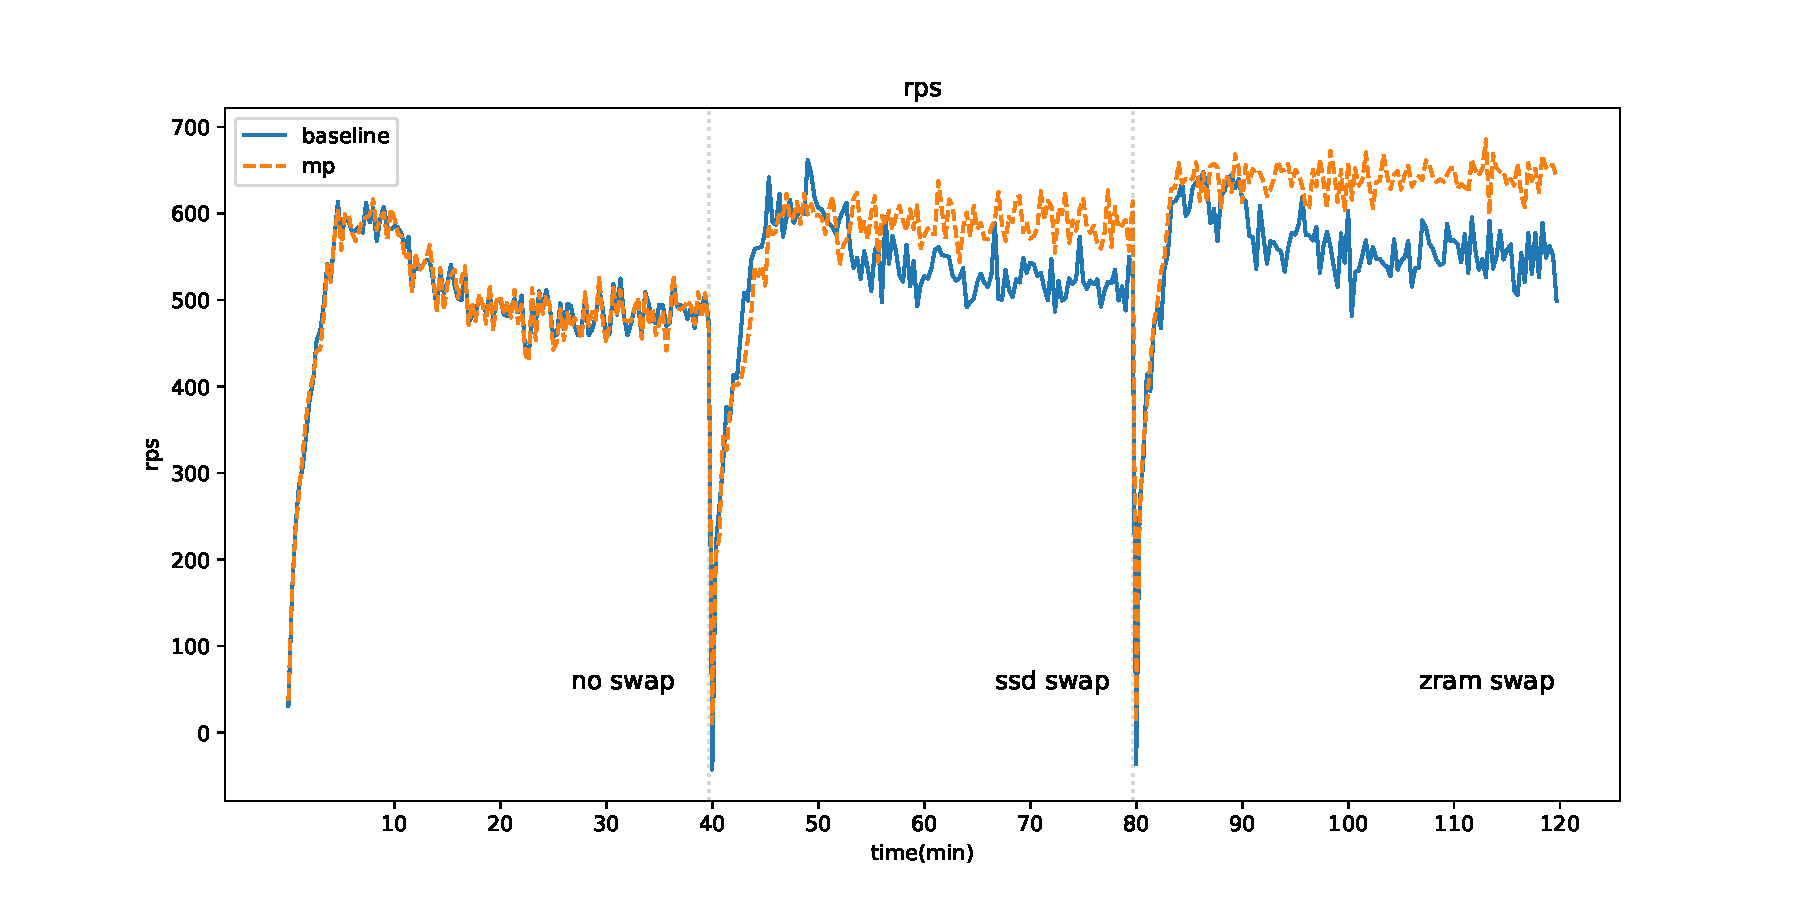
\includegraphics[width=\textwidth]{rps.pdf}
    \caption{Web Server 负载在多种场景下的 RPS 对比}
    \label{fig:rps}
\end{figure}

从内存使用角度而言,图\ref{fig:mem}展示了不同时刻系统实际占用的内存空间。禁止 \texttt{swap} 时的占用最为紧张,一旦工作集超出物理可用范围,性能会大幅波动。SSD \texttt{swap} 能在一定程度上释放物理内存,但幅度有限;zram 则借助压缩手段使得内存占用有明显下降。若配合自适应回收算法,系统会更积极地识别低频访问页面,并在合适时机将其卸载,从而在相同负载下保持更低的物理内存占用。值得强调的是 zram 场景的差异更为显著,说明当卸载后端访问成本较低时,内核会更加大胆地进行页面回收,以换取主内存空间的可用度。

\begin{figure}[htbp]
    \centering
    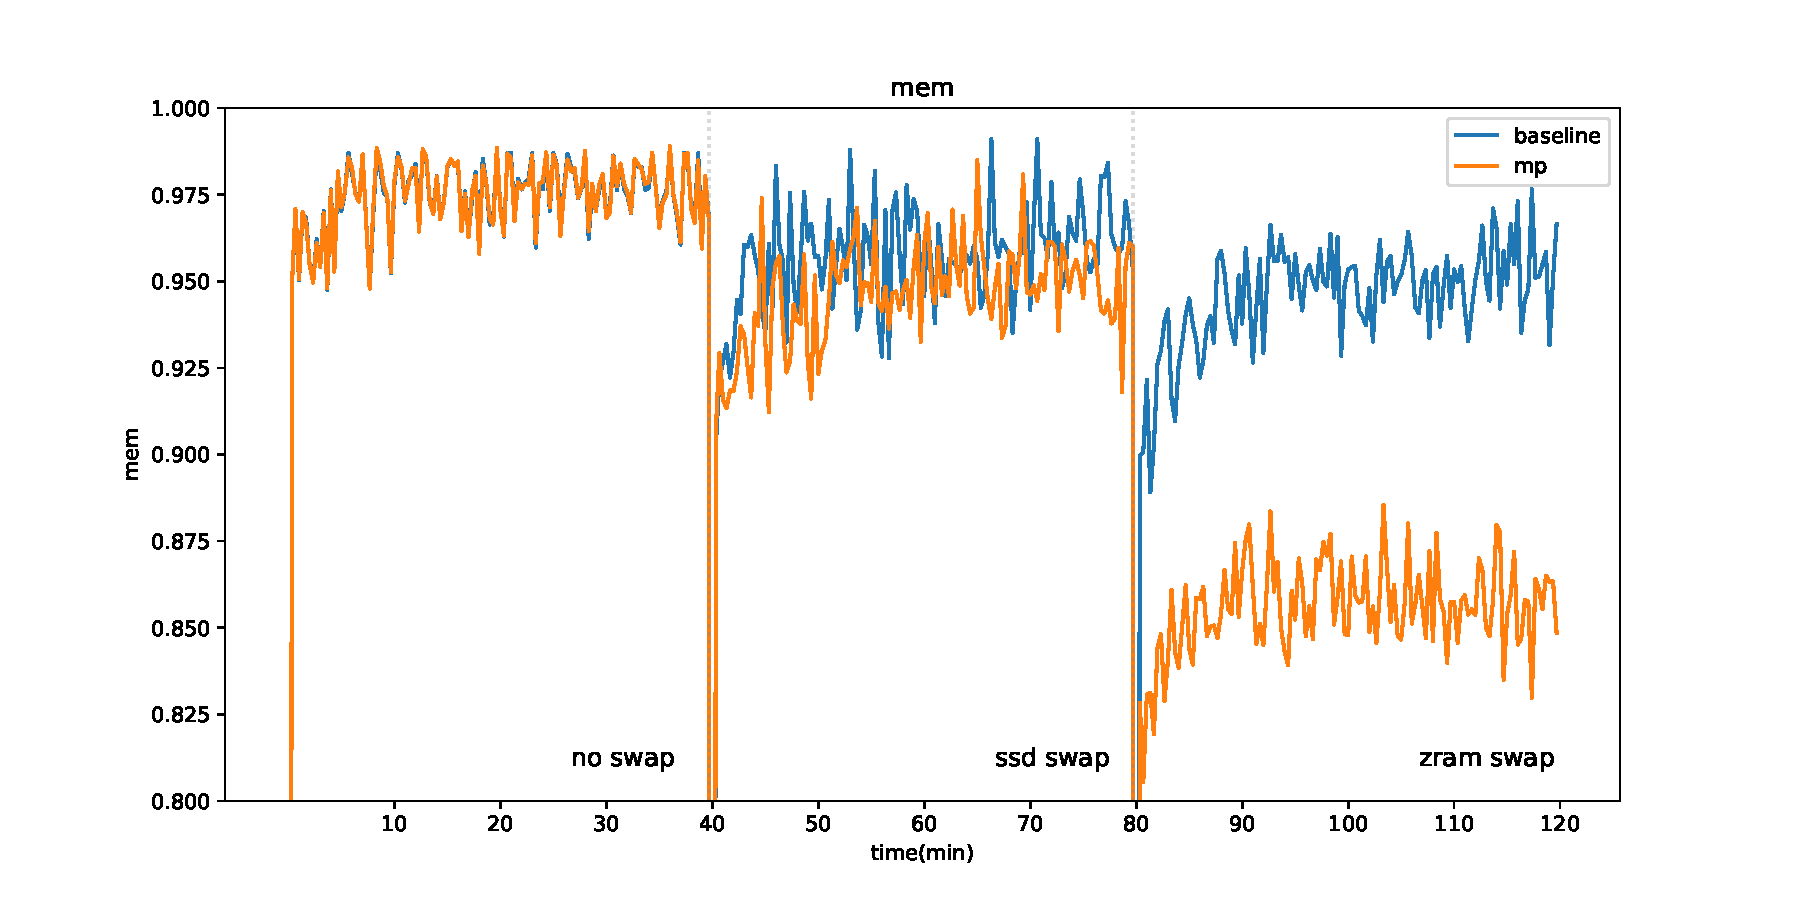
\includegraphics[width=\textwidth]{mem.pdf}
    \caption{Web Server 负载在多种场景下的内存使用对比}
    \label{fig:mem}
\end{figure}

在缺页中断次数方面,图\ref{fig:refault}显示了随着时间推移不同 \texttt{swap} 策略下的 refault 变化。zram 由于读写延迟远小于机械硬盘或常规 SSD,系统在侦测到其性能优势后往往会更积极地回收页面,一旦后续访问到已被回收的页面便会触发缺页中断,于是 zram 场景的 refault 次数偏高。表面上看这似乎意味着更多的页面换入操作,但其实际代价因为 zram 极低的访问延迟而相对有限,因此并不会对系统吞吐形成严重拖累。

\begin{figure}[htbp]
    \centering
    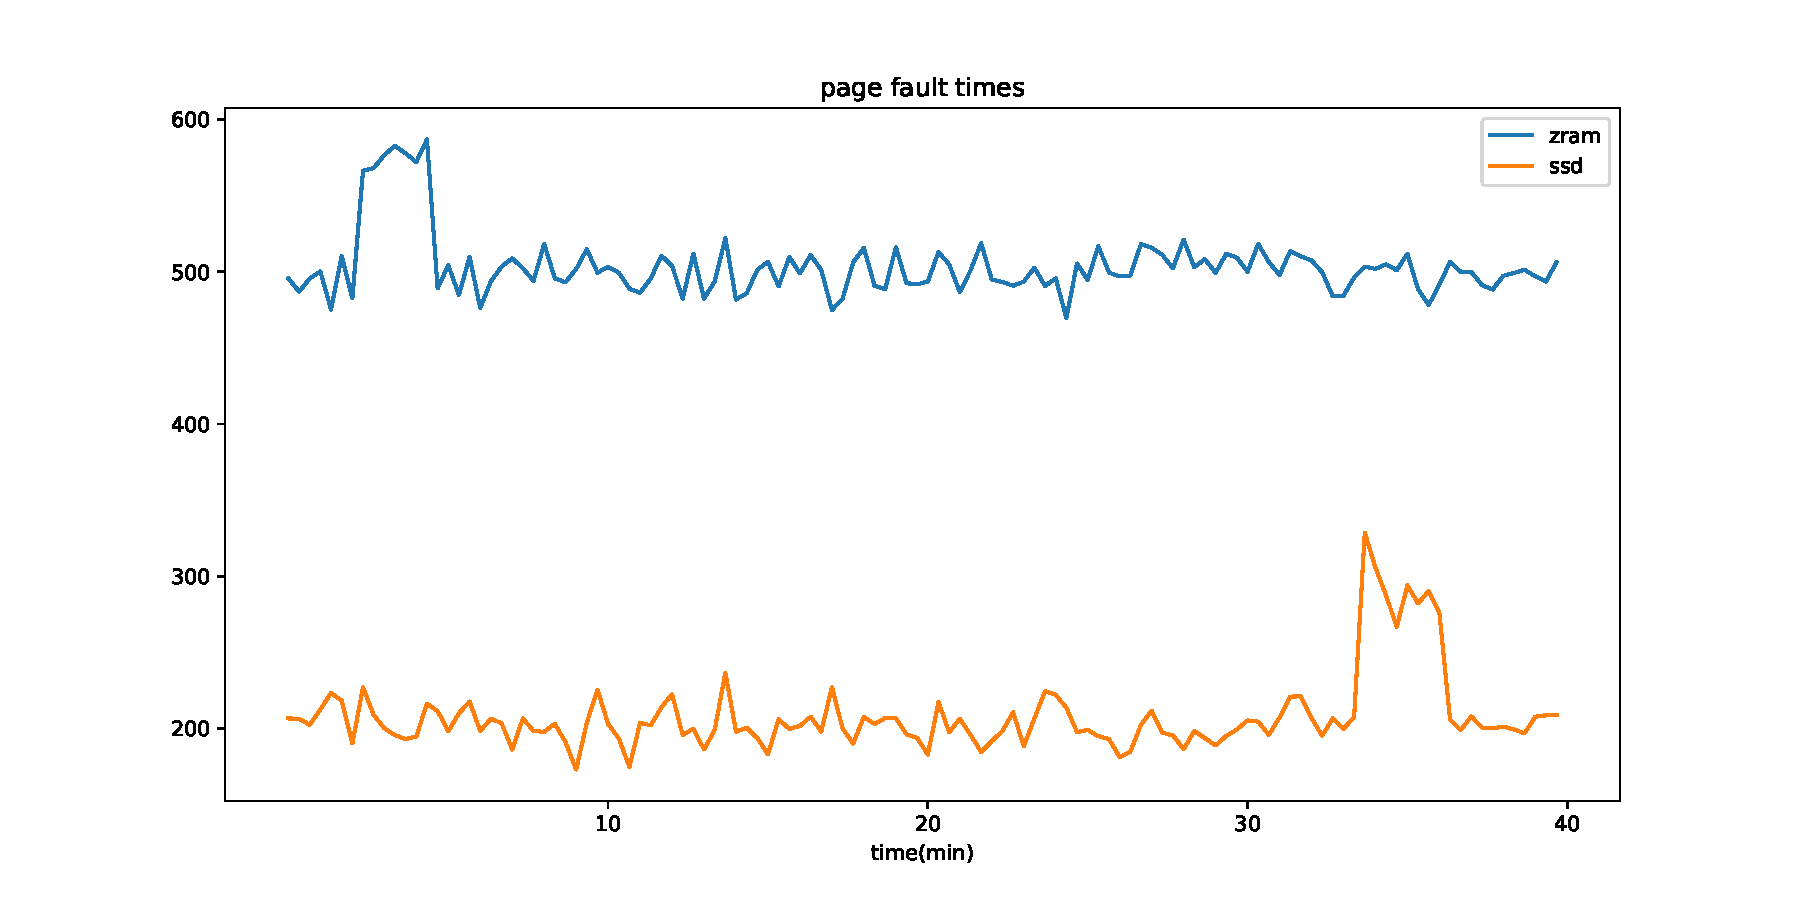
\includegraphics[width=\textwidth]{refault.pdf}
    \caption{Web Server 负载在多种场景下的缺页中断次数}
    \label{fig:refault}
\end{figure}

p90 响应时间如图\ref{fig:p90}所示,能够比较直观地体现系统在尾部延迟上的表现。可以看到在 SSD 作为卸载后端时,由于其 I/O 性能虽优于 HDD 但依旧是一个相对独立的外部存储介质,随机小块读写性能不及压缩内存,p90 相对略高且更易抖动;而 zram 场景在高压缩比与高吞吐特性下,能将尾部延迟维持在一个更低且更稳定的水平。当结合自适应算法后,zram 场景的 p90 再度下降,说明该算法可以及时识别并淘汰不活跃页面,从而降低了频繁换入对关键请求导致的尾部延迟。

\begin{figure}[htbp]
    \centering
    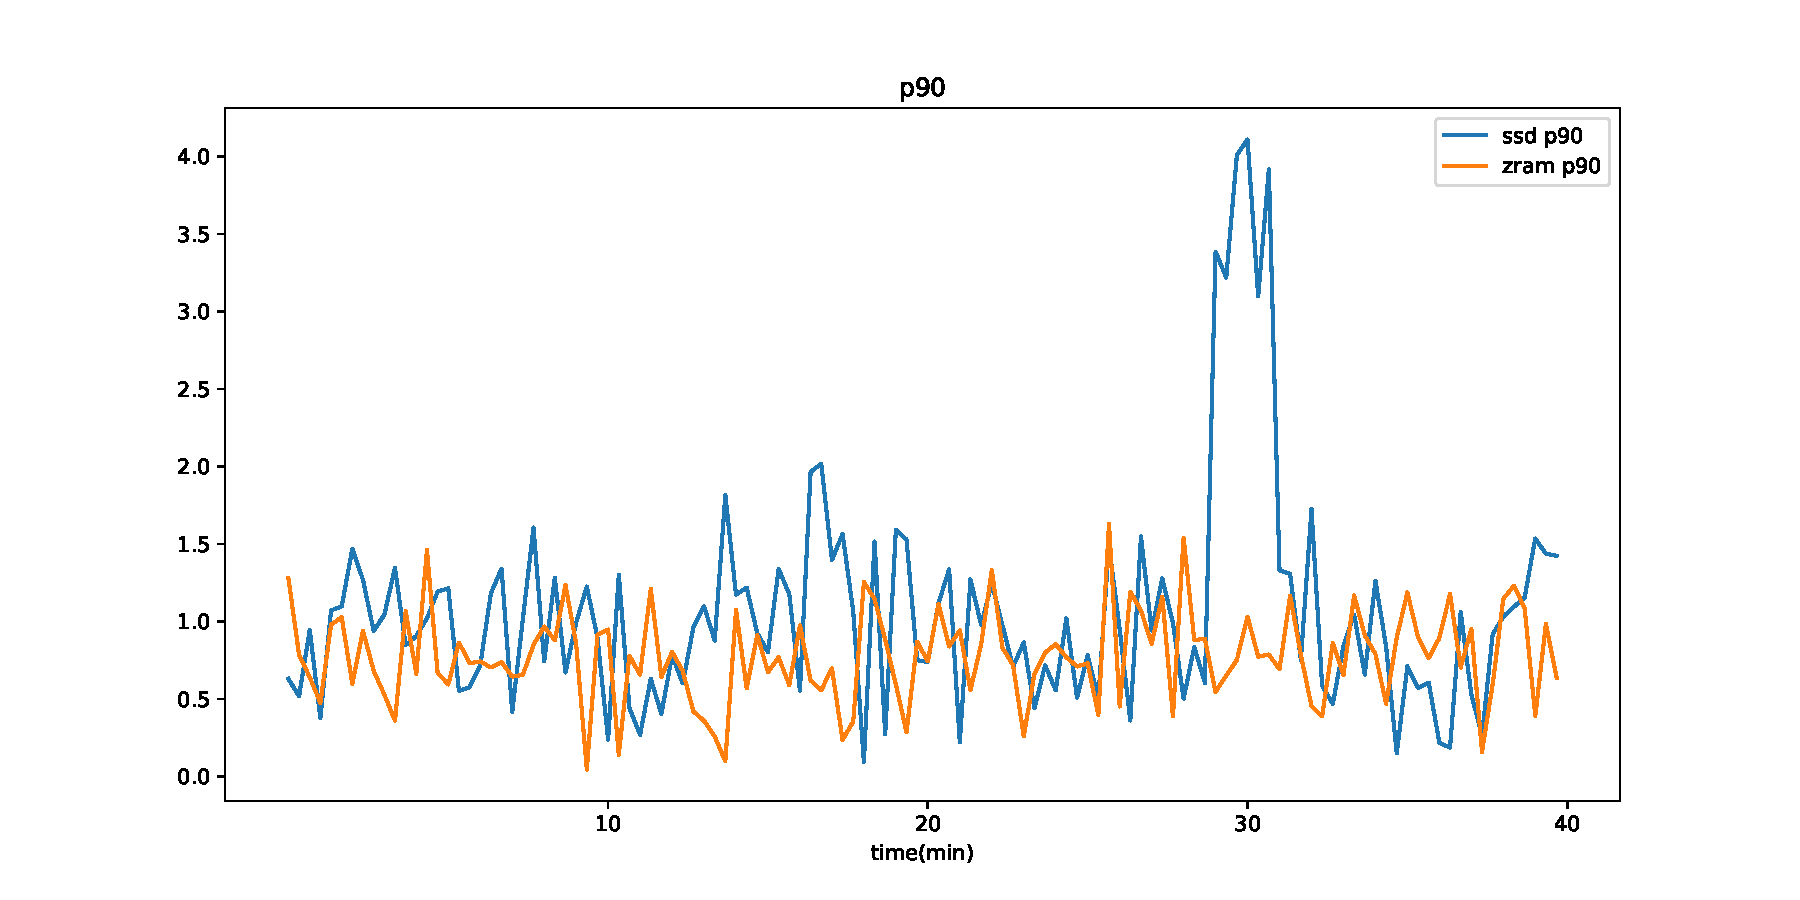
\includegraphics[width=\textwidth]{p90.pdf}
    \caption{Web Server 负载在多种场景下的 p90 响应时间对比}
    \label{fig:p90}
\end{figure}

最后,图\ref{fig:container_memory}展示了容器化场景下的实验结果,特别关注了当 Kubernetes 或类似系统为每个 Pod 创建顶层 CGroup 并在其中运行边车容器与业务容器时,整体内存使用的变化。随着容器数量规模的增长,边车容器在日志、流量代理和监控探针等方面产生的“虚拟化税”累积效应会日益突出。本研究在容器环境中同样利用内存压力模块与自适应回收算法对边车容器和核心负载容器进行同时检测,实测表明边车容器中相当一部分页面实际上是低频或不活跃数据,卸载到高性能介质(尤其是 zram)后可有效释放物理内存,从而将更多主内存资源留给核心负载,增强了集群整体的资源利用率与稳定性。

\begin{figure}[htbp]
    \centering
    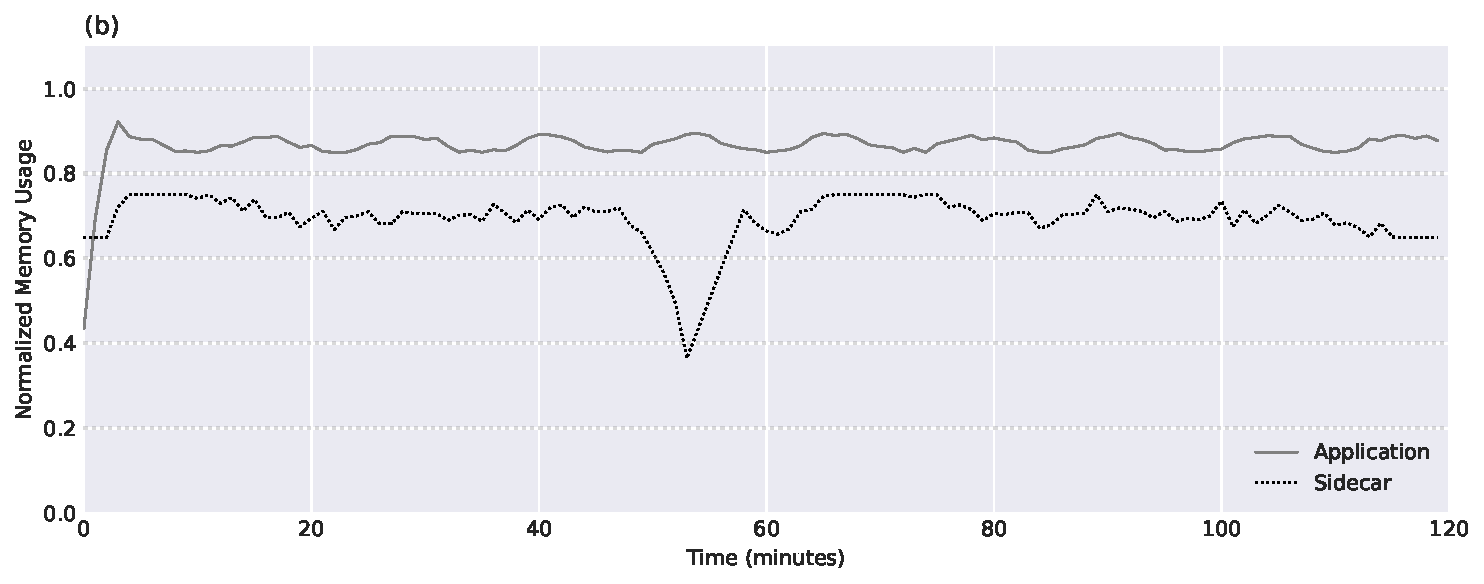
\includegraphics[width=\textwidth]{container_memory.pdf}
    \caption{自适应算法在边车容器与业务容器中的内存释放效果对比}
    \label{fig:container_memory}
\end{figure}

\section{本章小结}

通过本章一系列实验,可以得出以下主要结论:首先,本文所设计的内存压力模块能够在机械硬盘、SSD 和 zram 这三种卸载后端下有效触发和量化系统的内存压力,为后续回收算法提供真实的环境支撑。其次,文件页与匿名页均衡算法在文件密集型和内存密集型负载中均展现出良好的适用性,其针对 \texttt{swappiness} 的动态调节可避免过度回收缓存文件页或引发过度的匿名页换入换出,从而在不同场景里带来显著性能增益。再次,在综合测试中,结合内存压力与自适应均衡的整体方案能够高效地释放物理内存并在高负载时保持稳定的吞吐和延迟表现,其中 zram 作为卸载后端时展现了更加出色的性能。最后,在容器化场景下,边车容器的内存占用常常在实际部署中造成可观的资源浪费,通过在内核中实施基于压力的自适应回收机制,能够大幅降低这部分“虚拟化税”,在大规模服务环境下具有突出的应用价值。上述结论为下一步在更复杂或更大规模生产环境中推广这一内存回收与卸载方案提供了重要参考依据。

\chapter{全文总结与展望}

\section{全文总结}
本研究针对内存资源利用率优化的关键问题,在内存需求快速增长与内存扩展能力受限的背景下,提出了一种面向异构后端的自适应主动冷页面卸载方案。该方案通过优化Frontswap接口机制,实现了对异构卸载后端的自适应支持,并提出了基于内存压力的冷页面卸载策略以及基于重用的文件页与匿名页回收策略。具体而言,本研究的主要创新贡献可归纳为以下三个方面:

\begin{itemize}
    \item 提出了一种基于同步内存回收性能损失的内存压力量化方法。该方法通过精确测量内核处理同步内存回收操作的时间开销,有效屏蔽了用户负载和异构后端设备特性的差异性影响,解决了传统基于缺页率或页面分配次数等指标无法准确反映内存压力对应用程序性能实际影响的问题。实验结果表明,与传统方法相比,该量化方法能够更直接地反映内存压力对系统性能的负面影响,为冷页面卸载策略提供了可靠的决策依据。

    \item 设计了一种基于内存压力的冷页面自适应卸载策略。该策略通过将内存压力指标暴露至用户态,结合工作集大小预测机制和CGroup内存限制机制,实现了冷页面的动态卸载控制,从而在保证系统性能的前提下优化内存资源利用率。该策略的核心在于建立动态卸载量调整机制,有效避免了过度卸载导致的性能下降或卸载不足造成的资源浪费。实验验证表明,该策略能够实现内存使用效率与系统性能之间的最优平衡。

    \item 提出了一种基于重用的文件页与匿名页自适应回收策略。针对传统内核倾向于回收文件页的问题,该策略通过近似计算文件页的重用,自适应调整文件页与匿名页的回收比例,有效降低了同步内存回收操作导致的性能下降。该策略的创新之处在于引入重用量化指标,通过精确度量页面的访问频率与时间间隔,为回收决策提供了更准确的依据。实验结果证实,该策略能够显著降低因回收操作引起的性能波动,提升系统的整体稳定性。

\end{itemize}

\section{后续工作展望}
尽管本研究在异构后端环境下的主动冷页面卸载方面取得了阶段性成果,但仍存在若干关键问题需要进一步深入研究与优化:

\begin{itemize}
    \item 在文件页与匿名页回收策略的验证过程中,尚未实现匿名页重用的精确计算,这可能导致回收策略的准确性受到限制。后续研究将重点开发一种精确且高效的匿名页重用计算方法,进一步提高回收策略的精准度。

    \item 当前的冷热页面识别机制主要依赖于内核的Clock算法,该算法作为一种通用策略,未能充分考虑应用程序的优先级和访问特征。未来研究将探索基于eBPF(extended Berkeley Packet Filter)的冷热页面识别方法,通过捕捉应用程序的特定访问模式,实现更精确的冷热页面识别。同时,将研究如何结合应用程序的语义信息,进一步优化冷热页面识别的准确性,从而提升整体方案的性能。

    \item 当前的冷页面主动卸载方案主要针对硬件的延迟和带宽进行了自适应估计,屏蔽了异构卸载后端的速度差异,但尚未充分考虑异构卸载后端的特性差异。后续研究将重点解决NVM的写入优化问题以及CXL的cacheline级别内存访问等关键技术挑战。

\end{itemize}

以上问题的解决将进一步完善本研究的主动冷页面卸载方案,为内存资源的高效利用提供更可靠的技术支持,同时为未来内存管理技术的发展提供新的研究方向。
%\chapter{template}
This is the template of the chapter in split file.

\section{s1}
This is a section.

\subsection{sub1}
This is a subsection.

% misc

\thesisacknowledgement
在攻读博士学位期间,首先衷心感谢我的导师XXX教授

% 
\thesisappendix

\chapter{中心极限定理的证明}

\section{高斯分布和伯努利实验}

% Uncomment to list all the entries of the database.
\nocite{*}
\thesisbibliography{reference}

%
% Uncomment the following code to load bibliography database with native
% \bibliography command.
%
% \nocite{*}
% \bibliographystyle{thesis-uestc}
% \bibliography{reference}
%

\thesisaccomplish{publications}
% 
\thesistranslationoriginal
\section{The OFDM Model of Multiple Carrier Waves}


% 
\thesistranslationchinese
\section{基于多载波索引键控的正交频分多路复用系统模型}



\end{document}
